\documentclass{template}
\usepackage{graphicx,parskip,bibunits,appendix,float, csvsimple}
\usepackage[ruled] {algorithm2e}
\usepackage{listings}
\usepackage[usenames,dvipsnames]{color}
\usepackage[margin=0.5in]{geometry}
\usepackage{url,amsmath,amssymb,fancybox,listings,pdfpages,caption,multicol,datetime,rotating, booktabs, subcaption}
%\usepackage[usenames,dvipsnames]{color}
\usepackage[pagebackref=false,pdffitwindow=true]{hyperref}

%NOTE: The hyperref usepackage should be the last \usepackage!!
%NOTE: When pagebackref=true an error will appear at the end of compiling. press `q' to ignore
%NOTE: Referencing Algorithms does not work if this usepackage is before the hyperref include.!!
%NOTE: This is a comment, ignored when the document is compiled
%NOTE: The following document configuration settings generally do not need to be modified
%NOTE: More packages may need to be added to provide additional functionality

\hypersetup{
    pdftitle    = {Investigating Factors Affecting the
Classification of Successful Reddit Comments},
    pdfauthor   = {Murray Lyne, Andrew McLeman, Scott Thomson, Jordan Youngman, Joe McDonald},
    pdfsubject  = {Computer Science},
    pdfkeywords = {Reddit, Data, Classification, neural network, Text Mining, Social Media, cross-entropy},
    colorlinks  = true, anchorcolor = blue, filecolor = blue, urlcolor = blue,
    linkcolor   = blue,    %NOTE: change (blue) to (colIdentifier) to have links within the document in Black
    citecolor   = blue,    %NOTE: change (blue) to (colIdentifier) to have citation links within the document in Black
}

\definecolor{colBackGrnd}{rgb}{1,1,0.8}
\definecolor{colKeys}{rgb}{0,0,1}
\definecolor{colIdentifier}{rgb}{0,0,0}
\definecolor{colComments}{rgb}{0,.5,0}
\definecolor{colString}{rgb}{0,0,1}
\definecolor{colWhite}{rgb}{1,1,1}

\newcommand{\MyHookSign}{\hbox{\ensuremath\hookleftarrow}}

\newtheorem{Theorem}{Theorem}
\newtheorem{Proposition}[Theorem]{Proposition}
\newtheorem{Lemma}[Theorem]{Lemma}
\newtheorem{Proof}[Theorem]{Proof}
\newtheorem{Remark}[Theorem]{Remark}
\newtheorem{Claim}[Theorem]{Claim}
\newtheorem{Example}[Theorem]{Example}
\newtheorem{Definition}[Theorem]{Definition}

%NOTE: Setup for including program listings
\lstset{ 
  language=R,
  basicstyle=\tiny\ttfamily,      
  numbers=left,                   
  numberstyle=\tiny\color{Blue},  
  stepnumber=1,                   
  numbersep=5pt,                  
  backgroundcolor=\color{white},  
  showspaces=false,               
  showstringspaces=false,         
  showtabs=false,                 
  frame=single,                   
  rulecolor=\color{black},        
  tabsize=2,                      
  captionpos=b,                   
  breaklines=true,                
  breakatwhitespace=false,        
  keywordstyle=\color{RoyalBlue}, 
  commentstyle=\color{YellowGreen},
  stringstyle=\color{ForestGreen} 
} %\hypersetup{colorlinks=true, citecolor=\color{colIdentifier}}

\sloppy %NOTE: To ensure the Right Hand Margin is used (Especially for long URLS)
%NOTE: END of the document configuration settings

\begin{document}

\DeclareGraphicsExtensions{.jpg,.png,.gif,.pdf}
%NOTE: When inserting Figures if the extension of the graphic file is not provided LaTeX will automatically search
% for the extensions declared above, in the order declared.

\title{\huge{Investigating Factors Affecting the Classification of Successful Reddit Comments}}
\author{Group 6 - Andrew McLeman (1809076), Joe McDonald (1611267), Jordan Youngman (1607731), Murray Lyne (1607084), Scott Thomson (1508551)}
\degreetitle{MSc in Cyber Security} % Replace with appropriate degree
\rpttype{MSc}    % Replace MSc with BSc for Honours Degree Year projects.
\principaladviser{Eyad Elyan}

\beforeabstract
\prefacesection{Abstract}
Within the world of online marketing, the multitude of social media platforms that exist today serve as modern day market-squares, with the raucous cries of merchants replaced with a wall of text posts all competing for attention. The success of marketing material used on social media is heavily dependent on recognising the nuances of the targeted community, as well an understanding the psychological traits of social media users. A formula for achieving success on social media platforms would be extremely useful in allowing businesses to market their products in an effective manner. It would also be of great interest to the political sphere and would allow politicians to reach larger audiences and be able to appear more favourable to distinct voter demographics.

This report evaluates how the success of comments within the social media platform Reddit are affected by various extrinsic factors via a regression analysis.  The report also explores the content of each comment through text analysis and concludes by presenting a classification model, based on a neural network approach, to accurately determine how well-received a constructed comment would be within a chosen Reddit community.


\afterpreface \afterabstract

%\listofalgorithms   %NOTE: Will generate a list of Algorithms in the Table of Contents Section
%\lstlistoflistings  %NOTE: Will generate a list of Program Listings in the Table of Contents Section

%NOTE: Include the relative reference for each chapter to be included
% dividing the thesis file structure into a number of directories aids development
% format: directoryName/filename (the .tex extension is not required for the filename)

\chapter{Introduction}
\pagenumbering{arabic} \setcounter{page}{1}

A short paragraph introducing the topic the chapter examines.


\section{Background}

A number of pages about the background of the project.

\section{About this Thesis}
This is the thesis of \emph{Insert Full Name Here}, submitted as part of the requirements for the degree of MSc Computing: Software Technology at the School of Computing, Robert Gordon University, Scotland.

A number of paragraphs detailing the main expectations of this body of work.


\section{Conclusion}
A short conclusion summarising the chapter.

\chapter{Background Research}\label{ch:Background}

This chapter provides some background research on the project and examines some previous work.

\section{Political Motivations behind Subreddits}
Reddit is home to several political subreddits, many of which have high subscriber counts and activity per day. As stated in the paper titled Automating power political actors have used bots in social platforms to influence public opinion. They are used to not only raise awareness in certain political campaigns but also to follow politicians on platforms such as twitter and Facebook to give the illusion of popularity. They can even do an attack on news outlets where they flood their wall with misinformation as to avoid and sidetrack public attention. [10] the above research strongly shows why in our paper it is imperative that we distinguish AI from human users to get accurate and truthful data to work with. Also stated by the paper titled Melanization of Politics it describes and researches in the rise of political discussion due to the rise of media in the late nineteenth century early two-thousands it discusses how politics is now spoken on such a large scale. [11]

\section{Psychological Traits in Users}
Psychological traits play an important part in social media posts.

This paper[1] suggested that Users with Stronger personality traits tend to have stronger engagements in online discussions and therefore have increased interactions on Reddit. These users tend to use social media more because they have a more extroverted personality, and are much more open on social media platforms. This also means due to their extrovert traits, that these users tend to have better leadership qualities. The results, however, had issues with statistical significance.

Users tend to display “Cyborg-like” behaviour when trying to attract attention to their posts. This doesn’t always work and a significant number of posts studied [7] failed to garner the attention they wanted. 

\paragraph{User Behaviour Patterns}
It was found that women tend to post far less than men, and age determines how common a user will post on the platform. Users who had higher news engagement tend to comment and vote more on news related posts. As well as that, Older users were much more likely to post on Reddit.  Voting patterns have no significant predictors, with the only exception being that news engagement can predict voting. It was suggested that the reason women post less is due to the fear of suffering from online harassment, as Reddit has a history of harbouring subreddits that have “existed to only annoy other redditors”. Egregious examples include /r/fatpeoplehate and /r/rapingwomen. Of which, were banned by Reddit in 2015. [4]

When it comes to positive events occurring on Social Media, it was found that there is an increase in negative emotions in social media on Twitter. It was found that on Reddit, highly upvoted stories tend to gather a proportionate amount of downvotes, therefore indicating that the same effect can happen on Reddit as well.[3]

Most posts on Reddit “die” after one day in terms of activity, which is a pattern that has been observed on many other social media platforms. For posts that only had 1 posted comment, it was found that 72.78 Per cent of these post did not last more  600 seconds in terms of new activity [7]. Users who comment frequently on other user posts tend to have more highly scored posts and therefore if you want to have good interactions with other posts, you need to be reciprocative. 67 Per cent of authors had more effective comments than posts compared to 22 Per cent who has less effective comments than posts.

Most users are only active on a handful of subreddits. It was found that during a 1-year data collection on 309 Reddit users, only 109 unique users(104 subscribed and 44 unsubscribed) had subscription events fired (This is when a user subscribes to a subreddit). Users tend to have varying attention spans as 73 Per cent of posts are rated without viewing the content of the post first. It was found that most users were “headline browsers” who only look at the headline of a post before voting on it. It was also found that most users also only look at the top headline posts on the front page, which is known as position bias. This means that users tend to gravitate towards posts that are on top of the front page of a subreddit, compared to posts further down the page. Users often vote on posts before viewing the comments on the post. Over 50 Per cent of users vote before actually checking the comments replying to the post. [8]

It has been noted that the variety of subreddits browsed by users is lacking. A severe lack of browsing and voting variety was noted which indicates that users tend to create “echo chambers”, in which they only view content that they agree with. [8] This is a very commonly observed phenomenon across many social media platforms, and Reddit is no exception. [8]

Moderation doesn’t always affect user behaviour on Reddit. Subreddits themed around real-world discussion tend to value analytical and objective based comments compared to less serious subreddits. Even when filters are enabled preventing certain types of content being submitted, this makes little difference in the behaviour patterns of users.

\section{Significant Events}
Governments use bot farms on social media to manipulate public perception on social media, and Reddit is no exception. Many Governments, militaries and significant state actors have been outed as having used social-bots to appear either more relevant and influential or more controversially to directly manipulate legitimate users opinions on political events and military regimes. [5] 

\section{Machine Learning}
Reddit is host to multiple AI experiments as well as many bots to reply to incorrect post syntax. Reddit is commonly used due to having various different subreddits from politics down to humour subreddits. This makes for an excellent place for AI to learn through varying teaching methods such as reinforcement learning to learn from peers in the subreddit or to strive for higher upvotes then previous posts. [2]
The popularity of Reddit posts can be hard to classify without analysing the content of the post first. It can also be hard to classify posts if the subreddit in question covers a broad subject. Post popularity is determined on the content of the post, when the post was posted and the particular subreddit it was posted on, which, can be regarded as the context for discussion. An example of this would be the subreddit /r/pics, which had a poor performance in error rate due to the broadness of the subreddit’s context. Whereas other subreddits follow more specialized trends which are easier to classify. This paper ran classification algorithms and found that it ran better on simpler datasets. It also found that features like a Reddit post’s title lacked “indicative” power on whenever it made it a popular post or not. It suggested that more features from the Reddit API would improve prediction ability. [6]

With that said, this paper [9] suggests that it is possible to predict the score of Reddit comments, even if the communities are loosely defined (in terms of context) and disorganized. It found of note that user flairs (which are often given by moderators of a subreddit) can be an excellent predictor of highly popular comments. The model could also retrieve, with good precision, the highest rated comments within a particular post. It found that lowly rated comments tend to contain outdated jokes or information, which by that point had been cycled by the community to the point of exhaustion. Machine learning on Reddit needs to take into account community-related factors into what makes a comment popular. Posts on expertise related subreddit communities tend to use more technical and analytical terms. Likewise, comments on news related subreddits tend to be less emotional and value analytical insight over emotional responses. Some subreddits can vary in language use, the /r/worldnews subreddit is more diverse lexically, whereas /r/worldpolitics tends to use more “netspeak” compared to other subreddits. Emotional comment preference can vary between subreddits, with some subreddits heavily disliking having emotion in their comments. Time can play an important factor in determining how popular a comment can get. Comments on communities such as /r/news tend to be much more popular compared if posted later in time compared to comments made earlier, whereas other communities show the opposite happening. Moderation doesn’t always affect user behaviour on Reddit. Subreddits themed around real-world discussion tend to value analytical and objective based comments compared to less serious subreddits. Even when filters are enabled preventing certain types of content being submitted, this makes little difference in the behaviour patterns of users. This means that moderation doesn’t necessarily need to be taken into consideration when ranking comments, as the user behaviour is always affected by a significant amount.


\section{Conclusions}

The main conclusions for this chapter.

\chapter{Method}\label{ch:Method}



\section{Conclusions}





\chapter{Results}\label{ch:Results}

\section{Linear Modelling}

\subsection{Length of Comment vs Comment Score}
    The first potential linear relation that was examined was to see if the length of the comment could be used as a predictor of the score of the comment. The length of the comment was measured based on the number of characters within the \textit{body} field of the comment. Firstly a simple graph was plotted of the score of each comment vs the length of the comment, this can be seen in \autoref{fig:scorevlen} below. This proved to be extremely unhelpful due to the fact that there are so many comments with a score of 0, which is unclear in the plot.
    
    \begin{figure}[H]
        \centering
        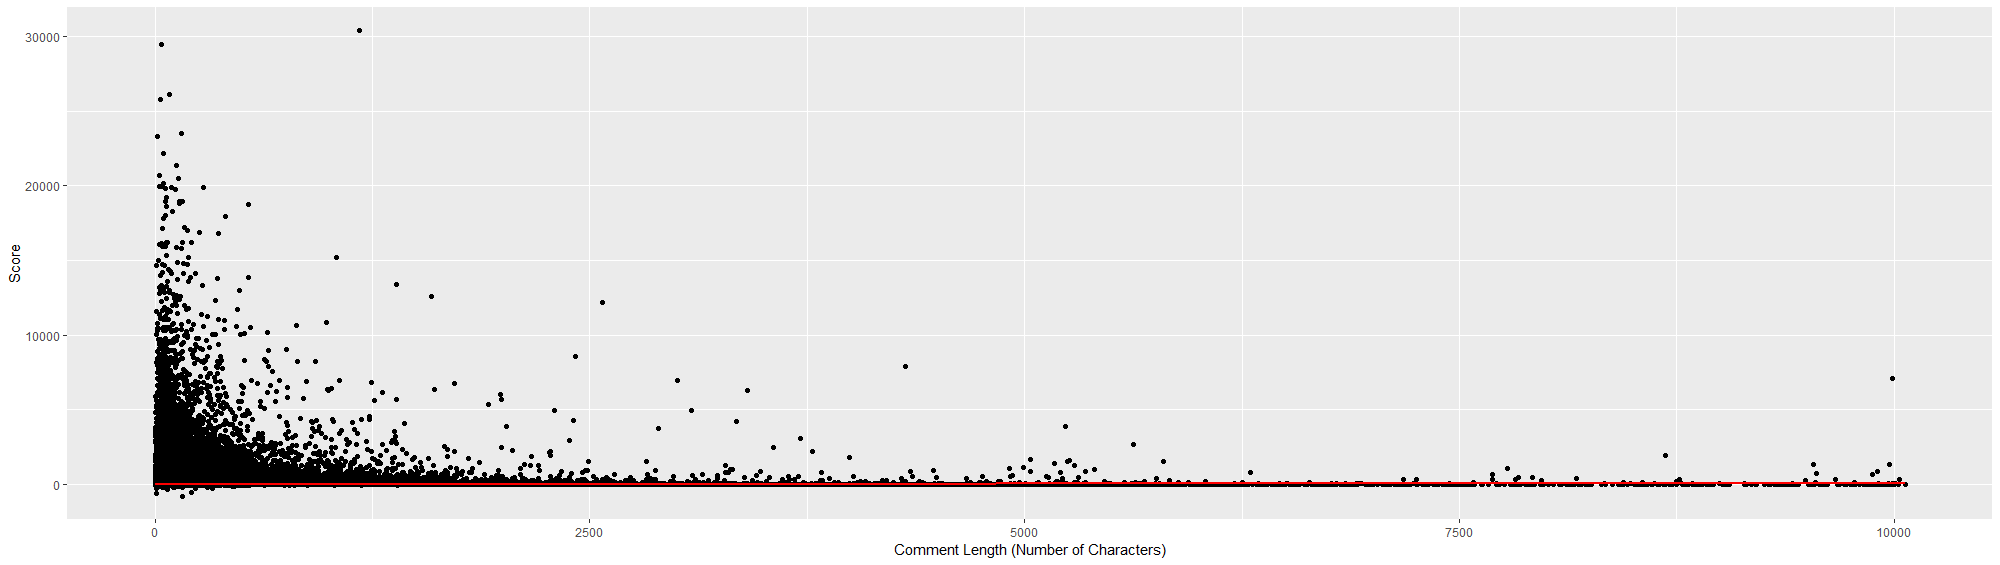
\includegraphics[width=1.0\textwidth]{graphs/length_score_all_subs}
        \caption{\textit{Length of comment versus the score}}
        \label{fig:scorevlen}
    \end{figure}
    
    A second attempt was made but this time the data was transformed to show the percent of successful comments at each particular length. The data was also grouped into 10 character chunks to help remove outliers. This new plot is shown in \autoref{fig:lenvscore} and \autoref{fig:lenvscore2} below.
    
    \begin{figure}[H]
        \centering
        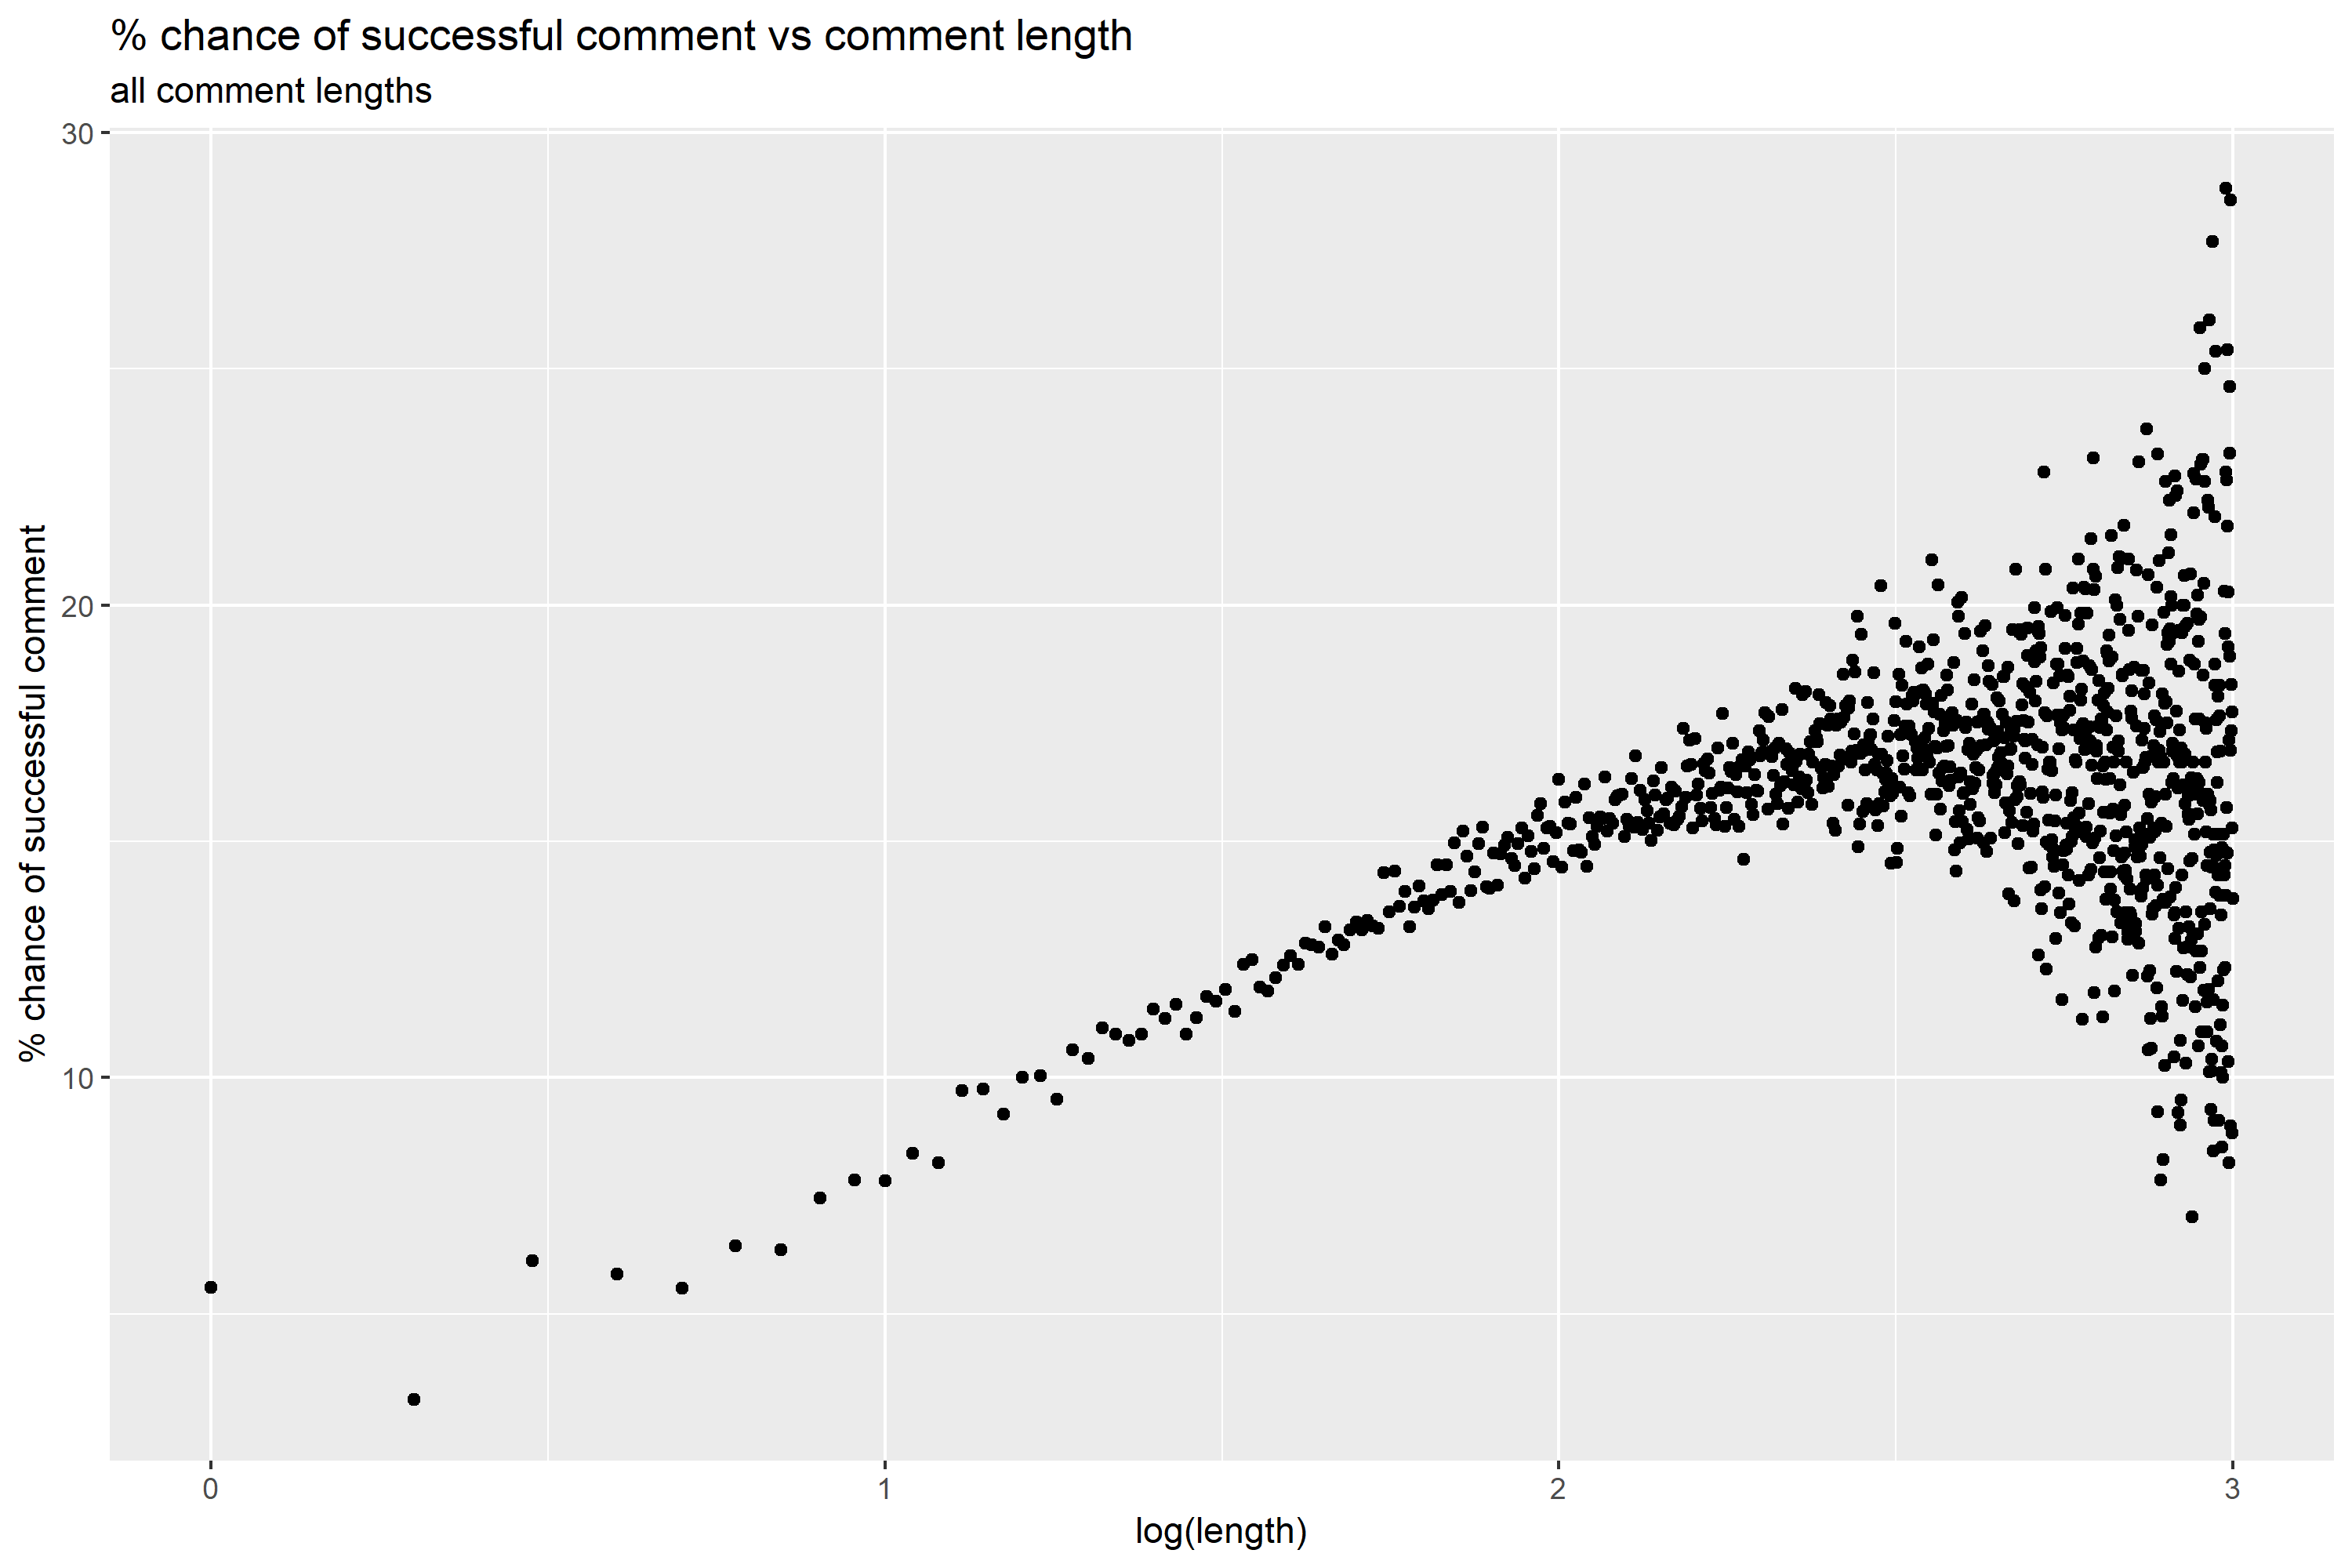
\includegraphics[width=1.0\textwidth]{graphs/lengthvsscore.png}
        \caption{\textit{Average score vs length where length is in 10 character chunks}}
        \label{fig:lenvscore}
    \end{figure}
    
    \begin{figure}[H]
        \centering
        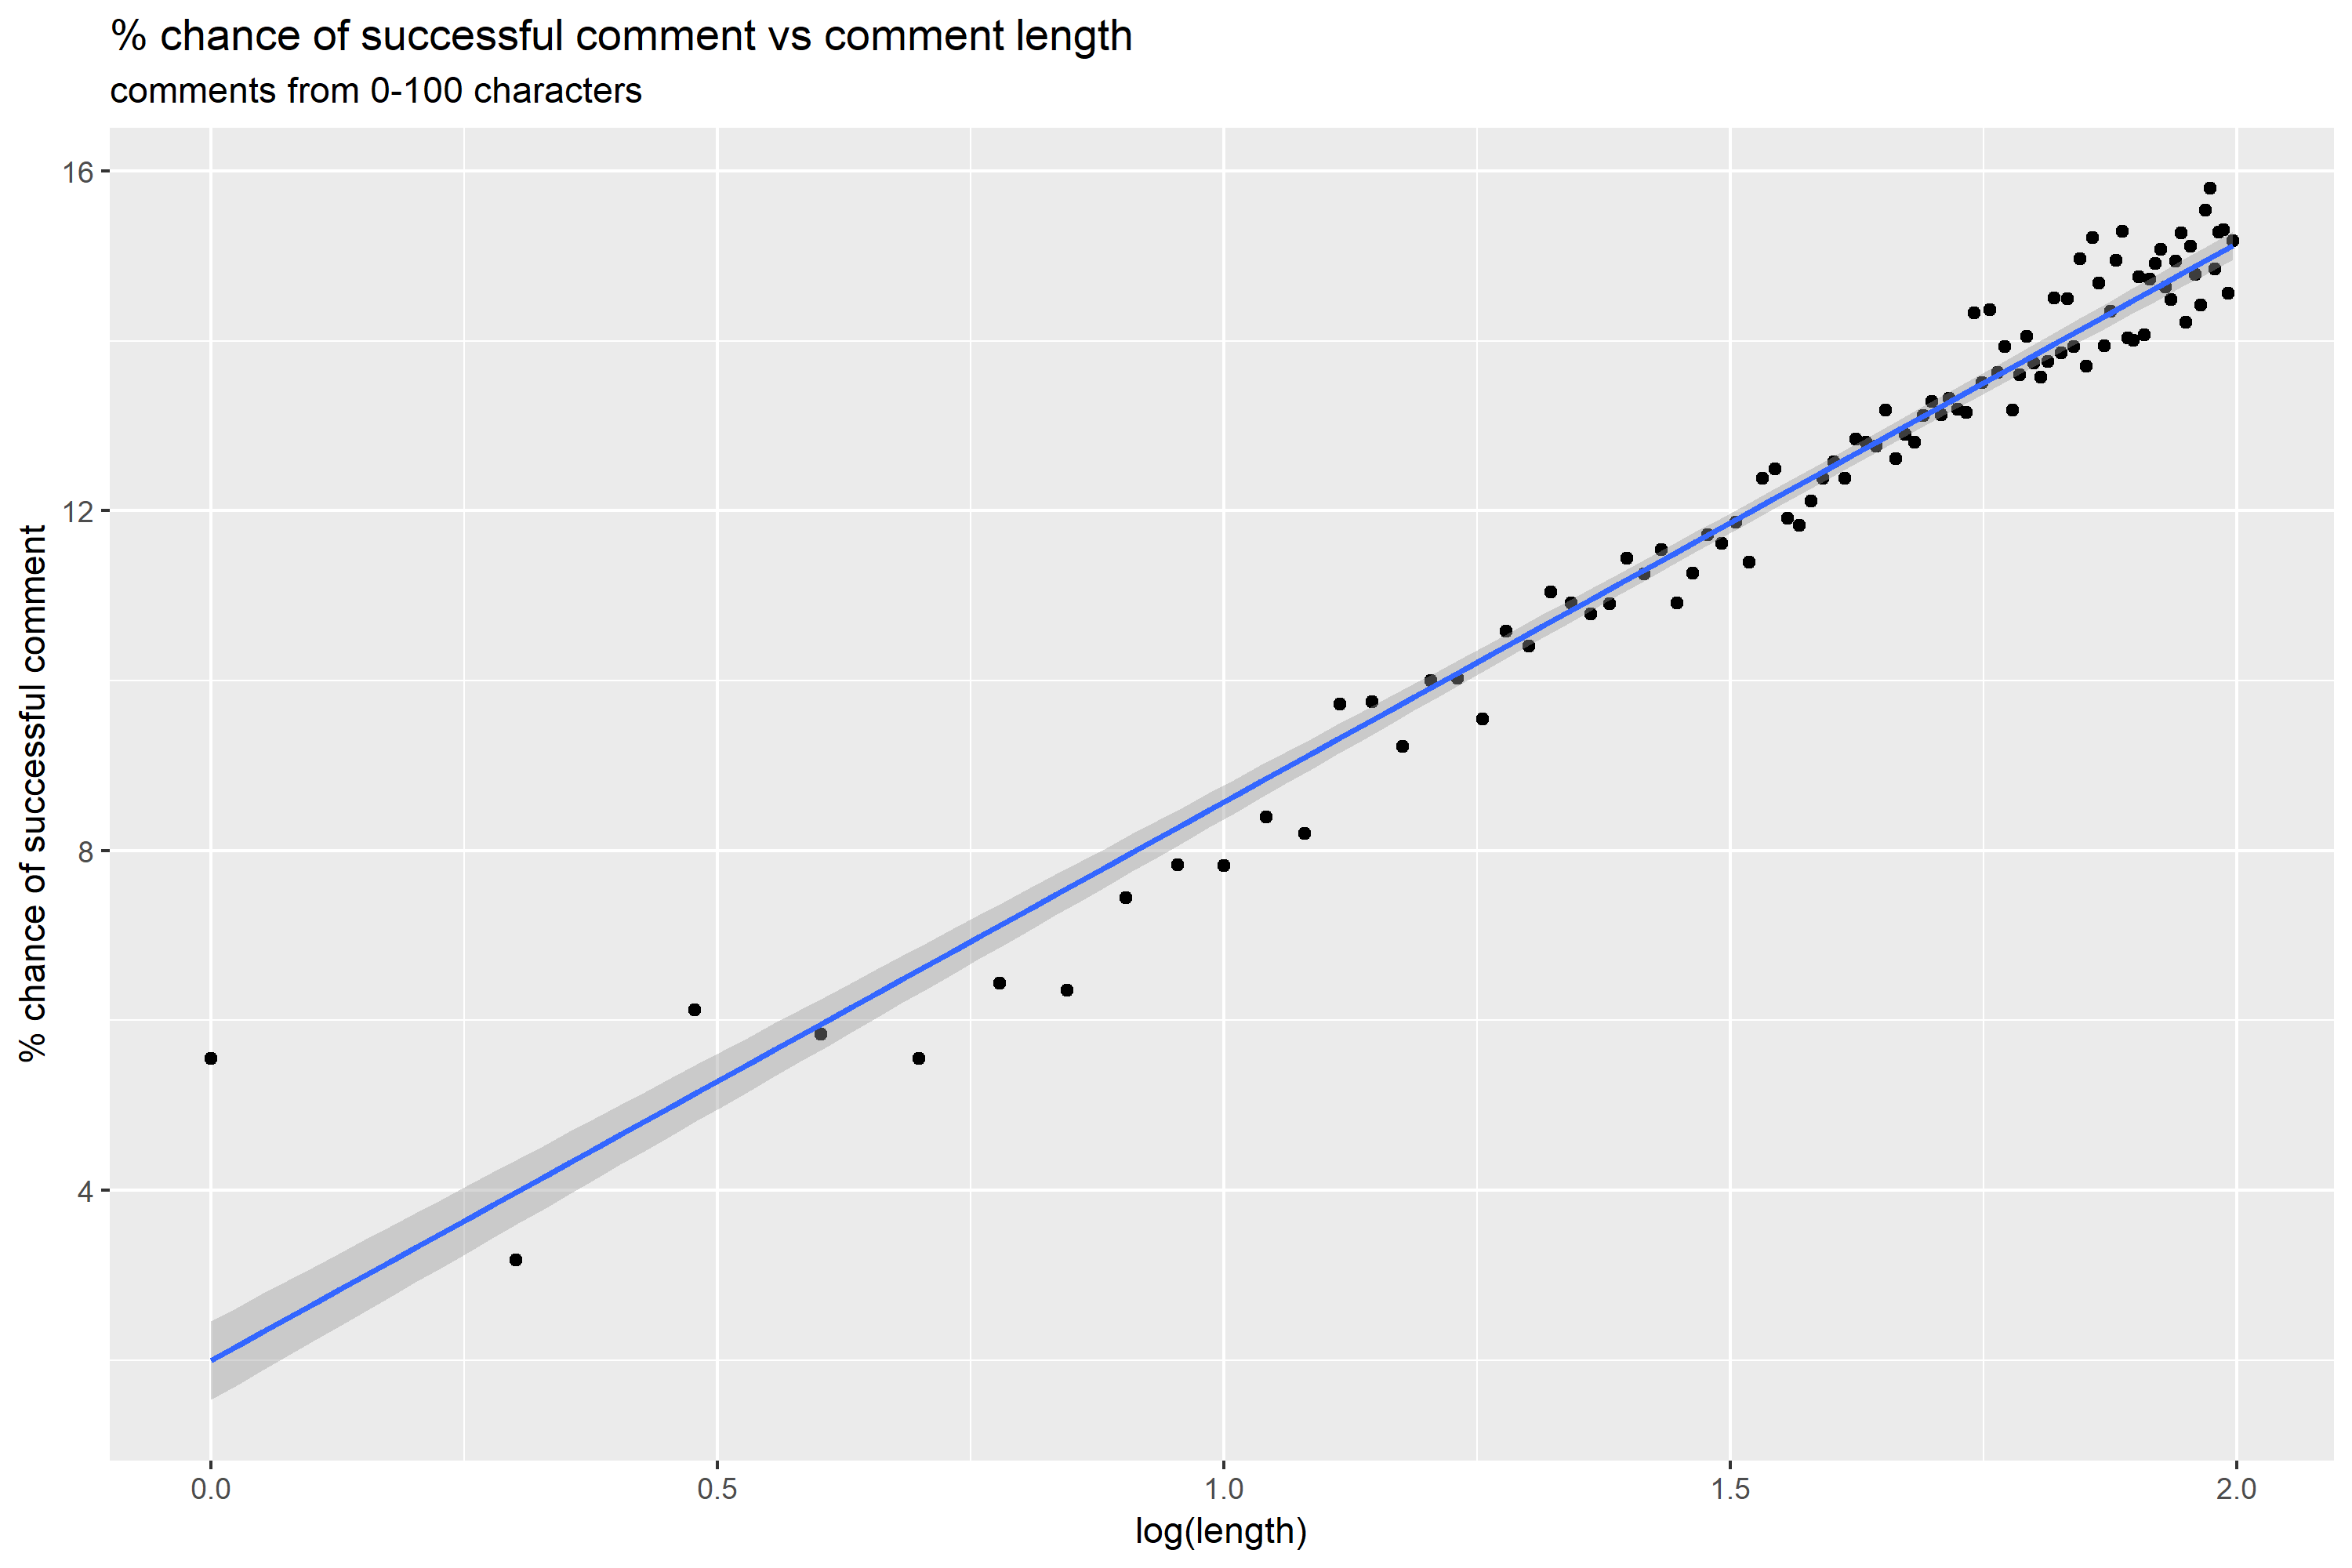
\includegraphics[width=1.0\textwidth]{graphs/lengthvsscore2.png}
        \caption{\textit{Same as \autoref{fig:lenvscore} but filtered to comments under 100 characters}}
        \label{fig:lenvscore2}
    \end{figure}

    Interestingly \autoref{fig:lenvscore} displays a linear relationship between length and score up to a length of around 100 characters, after which the score becomes unpredictable. It is believed that this is due to the lack of comments which exist at these lengths. \autoref{fig:lenvscore2} is the same plot but focused solely on the trend up to 100 characters, clearly indicating a linear relationship.
    
    The summary of this relationship is shown in \autoref{fig:lenvscoresum} below.
    
    \begin{figure}[H]
    \begin{lstlisting}
    Coefficients:
            Estimate Std. Error t value Pr(>|t|)    
(Intercept)  1.28544    0.18612   6.907 5.39e-10 ***
log(length)  3.04051    0.04947  61.462  < 2e-16 ***
---
Signif. codes:  0 ‘***’ 0.001 ‘**’ 0.01 ‘*’ 0.05 ‘.’ 0.1 ‘ ’ 1

Residual standard error: 0.4169 on 96 degrees of freedom
Multiple R-squared:  0.9752,	Adjusted R-squared:  0.975 
F-statistic:  3778 on 1 and 96 DF,  p-value: < 2.2e-16
    \end{lstlisting}
    \caption{\textit{Summary of the linear model from \autoref{fig:lenvscore2}}}
    \label{fig:lenvscoresum}
    \end{figure}
    
The code used to produce these graphs and summary can be found in \autoref{ch:Appendix} \autoref{sec:AppendexA6}


\subsection {Average Score vs Time Since Post}
    Another possible linear relation that was investigated was how much the average score of a comment varied based on the age of the post it was commenting on. Analysis showed that comments which were posted earlier were much more likely to get a higher score. The mean score quickly decreased as time progressed before flat-lining at around 100 5-minute intervals, which is approximately 8 hours. This is shown in \autoref{fig: timesincepost} below.
    
    \begin{figure}[ht]
        \centering
        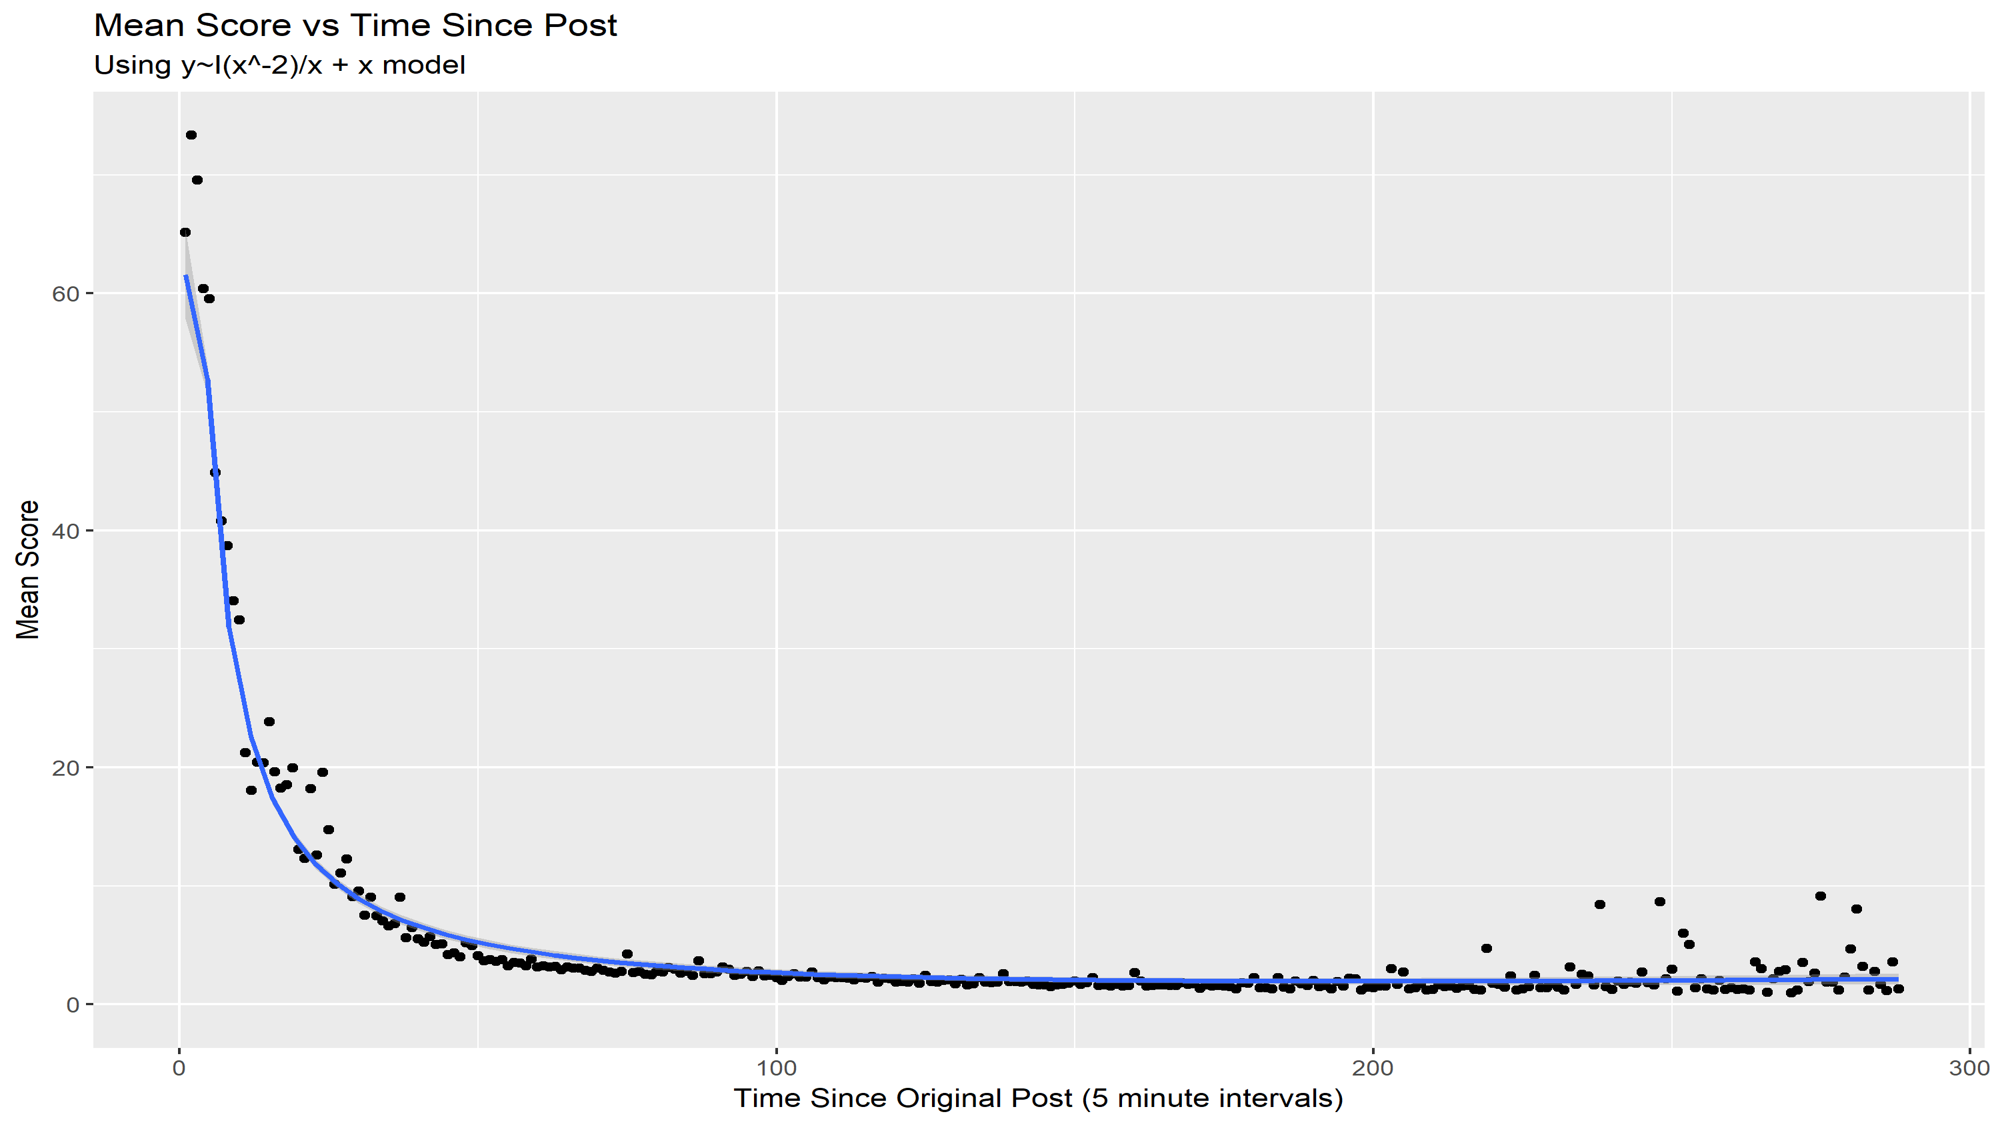
\includegraphics[width=1.0\textwidth]{graphs/meanscore_vs_time2}
        \caption{\textit{Mean Score versus time since post}}
        \label{fig: timesincepost}
    \end{figure}

It is clear from \autoref{fig: timesincepost} that the quicker a comment is created on a post, the more score it is expected to get. This conclusion is intuitive since earlier comments will be more visible to users visiting the comments section, and earlier comments will be seen by more users overall.

The summary of this relationship is shown in \autoref{fig:tspsum} below.

\begin{figure}[H]
    \begin{lstlisting}
Coefficients:
                Estimate Std. Error t value Pr(>|t|)    
(Intercept)      0.98419    0.09384   10.49   <2e-16 ***
I(dif^-2)     -217.18600    6.33142  -34.30   <2e-16 ***
I(dif^-2):dif  279.10738    5.21820   53.49   <2e-16 ***
---
Signif. codes:  0 ‘***’ 0.001 ‘**’ 0.01 ‘*’ 0.05 ‘.’ 0.1 ‘ ’ 1

Residual standard error: 2.752 on 953 degrees of freedom
Multiple R-squared:  0.8086,	Adjusted R-squared:  0.8082 
F-statistic:  2013 on 2 and 953 DF,  p-value: < 2.2e-16
    \end{lstlisting}
    \caption{\textit{Summary of the linear model from \autoref{fig: timesincepost}}}
    \label{fig:tspsum}
    \end{figure}

The code used to produce these graphs and summary can be found in \autoref{ch:Appendix} \autoref{sec:AppendexA7}

\subsection {Comment Tier vs Average Comment Score}
The next linear relation that was investigated was how the average score of a comment varies with how far down the comment chain that the comment was. The plot and linear model for this is shown in \autoref{fig: meanscorevscommenttier} below.

 \begin{figure}[H]
        \centering
        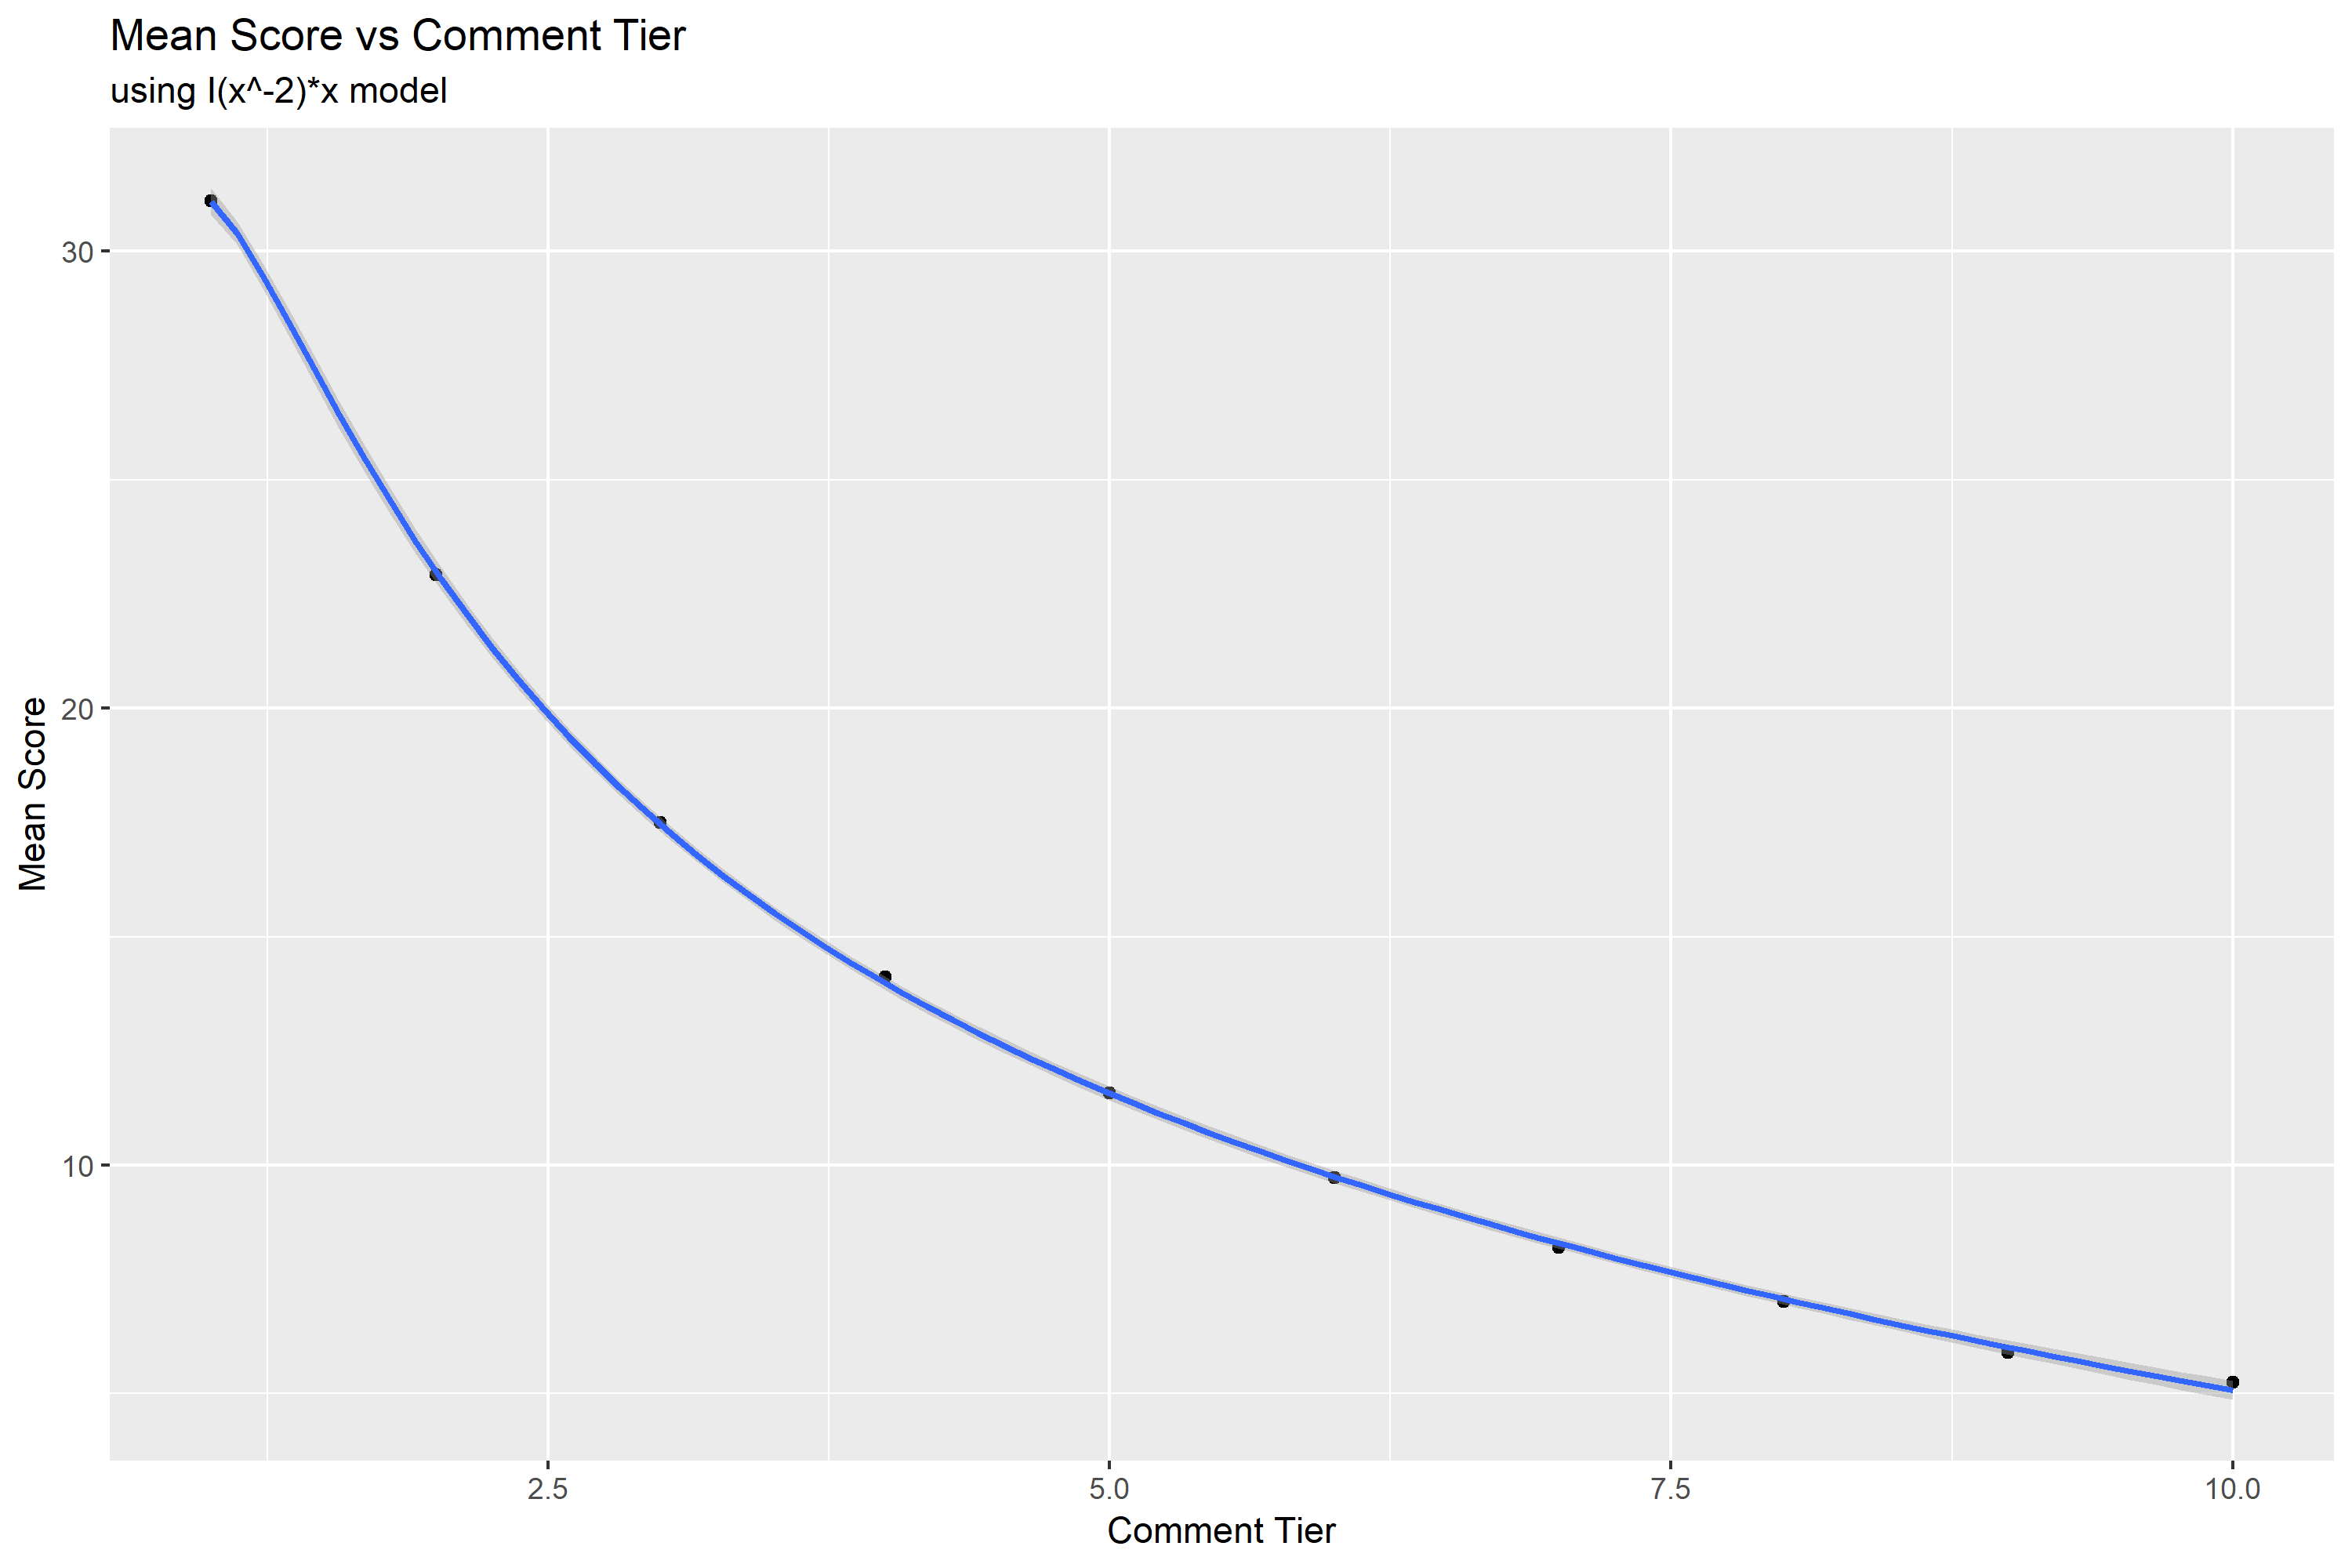
\includegraphics[width=1.0\textwidth]{graphs/meanscorevscommenttier.png}
        \caption{\textit{Mean Score vs Comment Tier}}
        \label{fig: meanscorevscommenttier}
    \end{figure}

As would be expected, the further down the comment tier a comment is, the less score it is expected to achieve. The summary of the linear model used is shown in \autoref{fig:commenttiersum} below, and the code used to produce the plot can be found in \autoref{ch:Appendix} \autoref{sec:AppendexA8}.

\begin{figure}[H]
    \begin{lstlisting}
Coefficients:
                 Estimate Std. Error t value Pr(>|t|)    
(Intercept)       4.75229    0.55055   8.632 0.000133 ***
I(tier^-2)      -22.97098    1.19209 -19.269 1.26e-06 ***
tier             -0.44247    0.04607  -9.604 7.29e-05 ***
I(tier^-2):tier  49.74669    1.65659  30.030 9.05e-08 ***
---
Signif. codes:  0 ‘***’ 0.001 ‘**’ 0.01 ‘*’ 0.05 ‘.’ 0.1 ‘ ’ 1

Residual standard error: 0.1169 on 6 degrees of freedom
Multiple R-squared:  0.9999,	Adjusted R-squared:  0.9998 
F-statistic: 1.533e+04 on 3 and 6 DF,  p-value: 4.853e-12
    \end{lstlisting}
    \caption{\textit{Summary of the linear model from \autoref{fig: timesincepost}}}
    \label{fig:commenttiersum}
    \end{figure}
    
\subsection{Average Score vs Time of Day}
How the average score of a comment varied based on the time of day was also found for all days of the week. Even though no linear modelling was carried out on this specific data, it would still be extremely important information to know in order to try to maximise the score that a comment received. \autoref{fig: avgscorevstimeofday} below shows how the average score varied over the course of a day, for all days of the week.

 \begin{figure}[H]
        \centering
        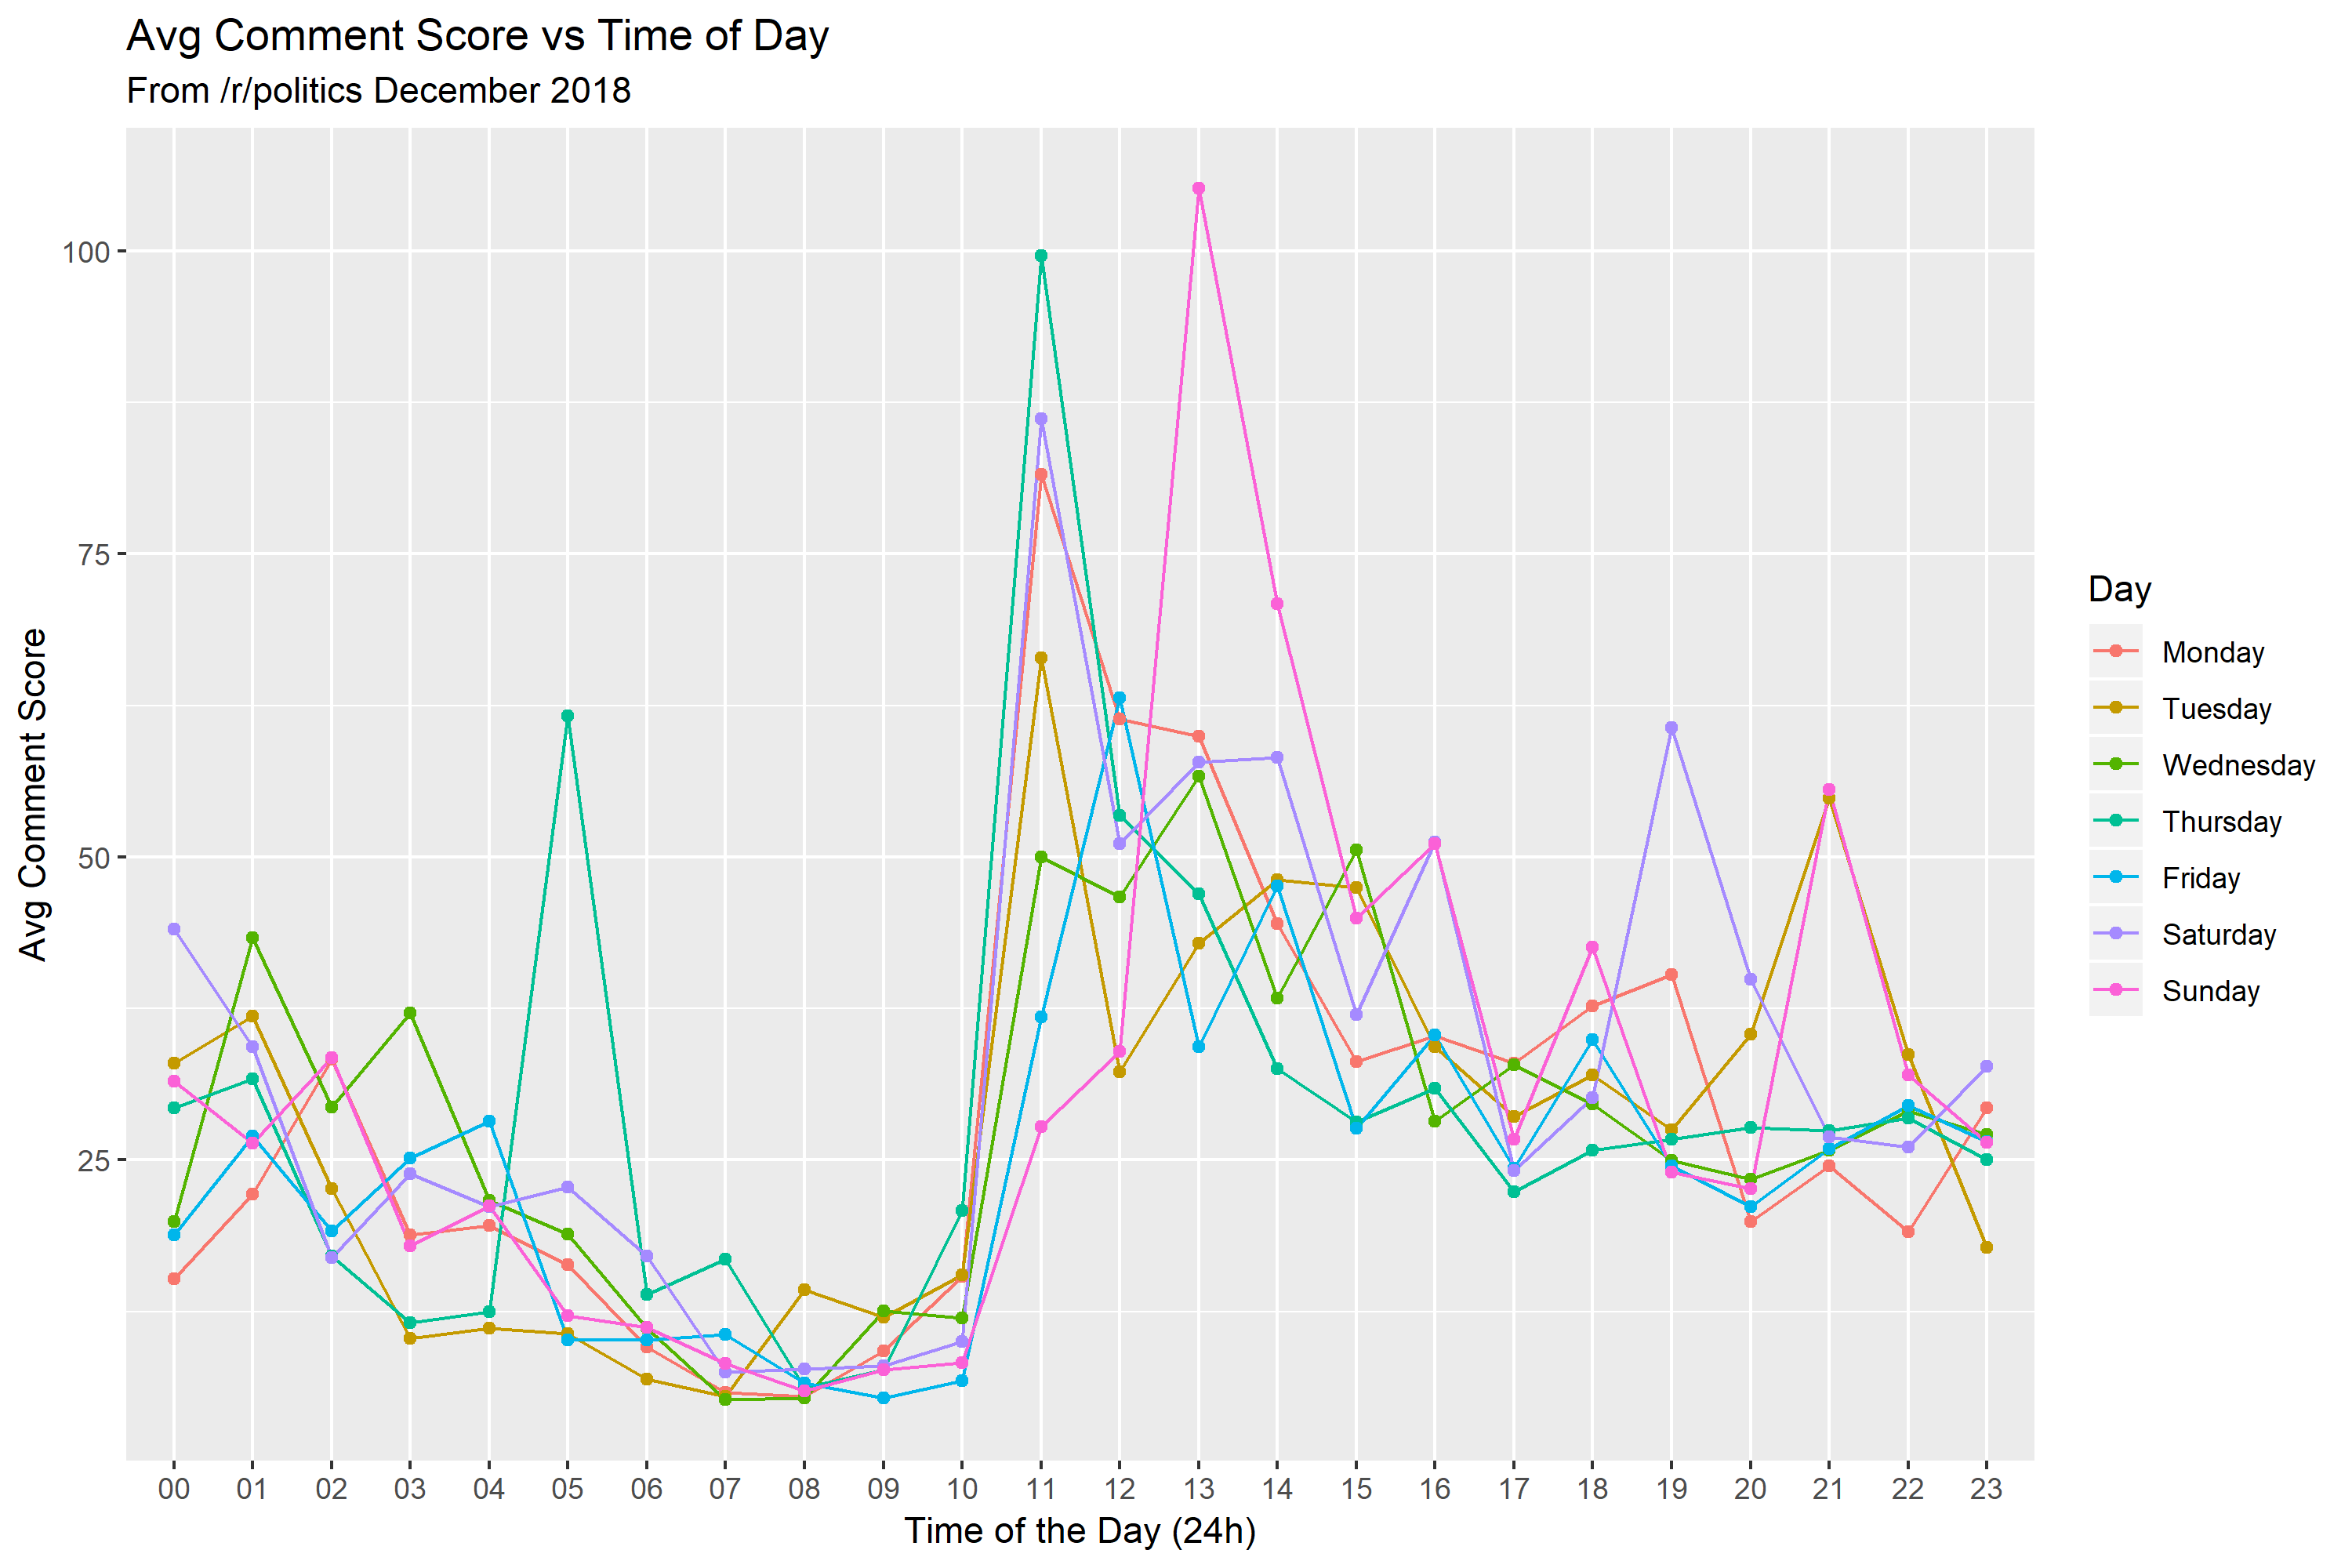
\includegraphics[width=1.0\textwidth]{graphs/avgscorevstimeofday.png}
        \caption{\textit{Average score over the course of the day for all days of the week}}
        \label{fig: avgscorevstimeofday}
    \end{figure}
    
As can be seen the average score is its highest around 12pm, and lowest around 9am, with weekends achieving overall higher scores. Thus to achieve the greatest chance of a high comment score, posting the comment midday at the weekend would give the highest chance of success. The code which generate the above plot can be found in \autoref{ch:Appendix} \autoref{sec:AppendexA9}

\section{Classification using a Neural Network}
\label{sec:NNclass}
Through attempts to generate a predictive model of score, it became clear the the words used within a comment were likely to be extremely important. However, it was not immediately clear how to best approach using text-analysis as a predictor. Simple models were initially made comparing the use of popular community words against score and no correlation was found. It was therefore decided to adopt a machine learning approach using the \textit{Keras} package as outlined in \autoref{sec:neuralnet}

The first neural network created simply took as input the words used within the body of a comment. These words were converted into a matrix as described in \autoref{sec:neuralnet} and used as an input for the neural network. Note, for this experiment, in an attempt to reduce the variables involved, only tier 1 comments were used. Due to this, the average score, which is an indicator of a comments success, had increased to 31 points. The training history of the first neural network attempt is shown in \autoref{fig:neural1} below.

 \begin{figure}[H]
        \centering
        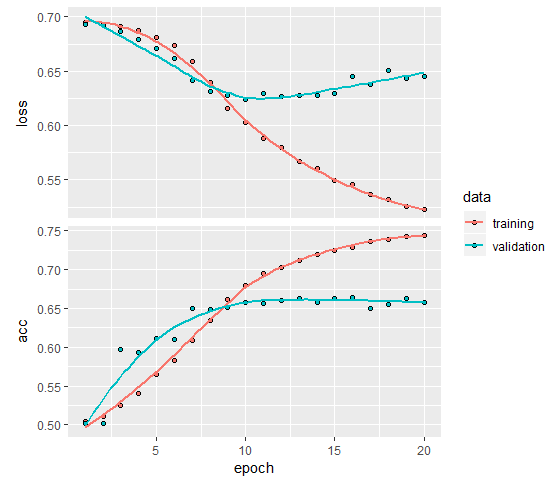
\includegraphics[width=1.0\textwidth]{graphs/neural1.png}
        \caption{\textit{History of a neural network of comment content. acc = accuracy}}
        \label{fig:neural1}
    \end{figure}

The neural network achieved a training accuracy of around 75\%, and a validation accuracy of around 66\%. This difference is due to the over-fitting of the data that occurs around epoch 9. Using the model as a predictor on a set of testing data revealed a classification accuracy of 67\%.

From an analysis of the data it was noticed that the topic of the post which the comment is in would be a powerful predictor of score. More popular post topics would attract more users, and thus comments within the post would achieve a higher average score. The above process of creating a neural network was repeated except the name of the post was extracted from the permalink field of the data. The words contained within the post name were then combined with the body and fed into the neural network again. The result of the training process is shown in \autoref{fig:neural2} below.

 \begin{figure}[H]
        \centering
        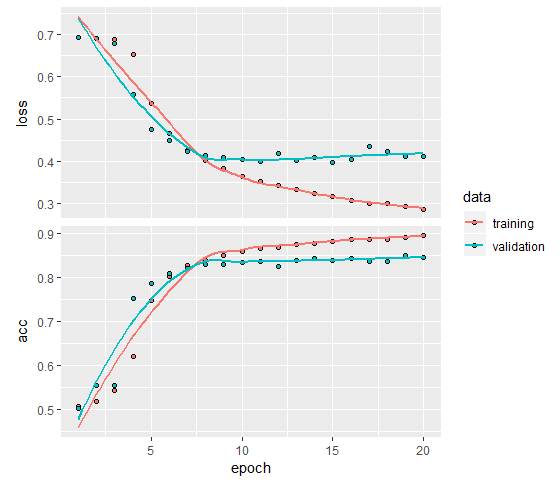
\includegraphics[width=1.0\textwidth]{graphs/neural4.png}
        \caption{\textit{History of the second neural network of comment content and post name}}
        \label{fig:neural2}
    \end{figure}

This new neural network achieved a training accuracy of 89\% and a validation accuracy of 85\%. Much like the first attempt it also experienced overfitting around epoch 9. When used on the same set of testing data as before, it achieved a classification accuracy of 84\%.

The code used to create this neural network is shown in \autoref{ch:Appendix} \autoref{sec:AppendexNeural}



\chapter{Conclusion}\label{ch:Conclusion}

This chapter summarises the main outcomes and conclusions resulting from this body of work.

\section{Conclusions}

The main conclusions that may be drawn from the body of work.

\section{Future Work}

Further development that could be carried out in the future.
\chapter{Project Management}\label{ch:Management}

\section{Tools used}
To organise team management related files, we used Google Docs\footnote{\url{https://docs.google.com/}} to write spreadsheets and draft documents. This benefited productivity because it was possible to edit these documents on any device with internet access. The service is also free of charge to use.

For team discussion and any meetings, the VoIP program Discord\footnote{\url{https://discordapp.com/}} was used for online discussion. Discord has built in features for automating team management, and despite being advertised for gaming hobbyists, it is a great alternative to Skype that is lightweight, does not require a client program and can be used on a web browser and is free to use. A Discord server was created to do any meetings and discussions, as well as used a web-hook extension for our GitHub to get real time updates on the GitHub repository used.

For writing R code, Git\footnote{\url{https://git-scm.com/}} was used to track changes across the script files. A private GitHub\footnote{\url{https://github.com/Medscootsman/RedditStudy}} repository was created to push changes to a centralised storage. As mentioned earlier, Discord's web-hook functionality was used to get real time information via a discord web-hook bot. This improved productivity and kept our work safe from any catastrophic accidents with our own devices. Production of R code was done on the RStudio IDE\footnote{\url{https://www.rstudio.com/}}.

For writing the report, we used RStudio in tandem with GitHub initially, however this proved to be prone to overwrite issues. To overcome this, Overleaf\footnote{\url{https://www.overleaf.com}} , a collaborative LaTeX editor was used. Overleaf made compiling the document very straightforward, and could be done automatically after every change. Premium features allowed users to track changes, though it was decided to use the free version due to the scope of the project.

\section{Team Meetings}
Please see \autoref{tab:meetings} for our meetings record. In summary, attendance was excellent and fruitful discussions on the project were held. Any time team members didn't show up there was valid justification for their absence.
\begin{table}[!ht]
    \centering
    \resizebox{\textwidth}{!}{
    \begin{tabular}{|c|c|c|c|c|c|c|c|}
         \bfseries Week & \bfseries Date & \bfseries Topic & \bfseries Andrew & \bfseries Joe & \bfseries Jordan & \bfseries Murray & \bfseries Scott
         \csvreader[head to column names]{tableData/meetings.csv}{}
         {\\\hline\week & \date & \topic & \Andrew & \Joe & \Jordan & \Murray & \Scott}
    \end{tabular}
    }
    \caption{\textit{Meetings record}}
    \label{tab:meetings}
\end{table}

\section{Peer Review Assessment}
Please see our peer review in \autoref{tab:peer}.
\begin{table}[ht]
    \centering
    \begin{tabular}{c|c|c|c|c|c}
         \bfseries Peer reviewer & \bfseries Andrew & \bfseries Joe & \bfseries Jordan & \bfseries Murray & \bfseries Scott
         \csvreader[head to column names]{tableData/peers.csv}{}
         {\\\hline\PeerReview & \Andrew & \Joe & \Jordan & \Murray & \Scott}
    \end{tabular}
    \caption{\textit{peer assessment}}
    \label{tab:peer}
\end{table}

\footnotesize  %NOTE: reduced the size of the text for the bibliography
%NOTE: set the style for the bibliography and display the references used within the document
\bibliographystyle{vancouver}
\bibliography{thesis}
\normalsize
\appendix
\chapter{Code Snippets}\label{ch:Appendix}
\lstset{ 
  language=R,
  basicstyle=\tiny\ttfamily,      
  numbers=left,                   
  numberstyle=\tiny\color{Blue},  
  stepnumber=1,                   
  numbersep=5pt,                  
  backgroundcolor=\color{white},  
  showspaces=false,               
  showstringspaces=false,         
  showtabs=false,                 
  frame=single,                   
  rulecolor=\color{black},        
  tabsize=2,                      
  captionpos=b,                   
  breaklines=true,                
  breakatwhitespace=false,        
  keywordstyle=\color{RoyalBlue}, 
  commentstyle=\color{YellowGreen},
  stringstyle=\color{ForestGreen} 
}

\section{Dataset parser}
\label{sec:AppendixParse}
\begin{lstlisting}
#include<iostream>
#include<fstream>
#include<string>
#include"rapidjson/document.h"
#include"rapidjson/writer.h"
#include"rapidjson/stringbuffer.h"
#include<chrono>

using namespace std;
using namespace rapidjson;

int main(int argc, char *argv[]){

	//Make sure that the user specificies a subreddit to parse.
	if(argc < 2){
		cout << "You need to specify the subreddit to parse" << endl;
		cout << "Syntax: ./subreddit_parser <subreddit name>" << endl;
		return 0;
	}

	string tempString = "";

	ofstream outputFile(argv[1] + string(".json"));

	//Create an interface to let the user see the progress
	auto startTime = chrono::system_clock::now();
	time_t start_time = std::chrono::system_clock::to_time_t(startTime);
	
	cout << endl << "Starting at " << ctime(&start_time) << endl;
	cout << "Parsing subreddit: " << argv[1] << endl;
	cout << "Will be saved to " << argv[1] << ".json in the current directory." << endl << endl;
	cout << "Completion:" << endl;
	cout << "0%---------------------------50%--------------------------100%" << endl;
	
	for(int i = 0; i < 122; i++){
		if(i % 2 == 0) cout << "|" << flush;
		ifstream inputFile("sample" + to_string(i) + ".json");

		while(getline(inputFile, tempString)){

			Document d;
			d.Parse(tempString.c_str());

			//Find the appropriate comments
			if(d["subreddit"] == argv[1]){
				outputFile << tempString << endl;
			}

		}
		inputFile.close();
	}
	outputFile.close();

	auto endTime = chrono::system_clock::now();
	time_t end_time = std::chrono::system_clock::to_time_t(endTime);
	
	cout << endl << endl << "Finished parsing at " << ctime(&end_time) << endl;

	return 0;
}

\end{lstlisting}

\section{Code to generated word clouds and word connection graphs}
\label{sec:AppedexFUNC}
\begin{lstlisting}
createGraphs <- function(data, subreddit, minimumCountLinks) {
  
  dataframe = as.data.frame(data.frame(User = data$author, 
                                       Date = as.POSIXct(data$created_utc, origin='1970-01-01'), 
                                       Comment = data$body,
                                       Score = data$score))
  
  print(count(dataframe))
  
  dataframe = subset(dataframe, User != "SavageAxeBot" & User != "KeepingDankMemesDank" & User != "AutoModerator" 
                     & User != "DankMemesMods" & User != "Colorizebot" & User != "BattleBusBot" & User != "MemeInvestor_bot" & User != "Transcribot"
                     & User != "Transcribot" & User != "commonmisspellingbot" & User != "TiltedTowersBot" & User != "stormshieldonebot"
                     & User != "WikiTextBot" & User != "RemindMeBot" & User != "thank_mr_skeltal_bot" & User != "societybot"
                     & User != "rick_rolled_bot" & User != "NoSkinBot" & User != "REEEEEEEEEpost" & User != "2Fdankmemes" & User != "deleted" & User != "GlobalOffensiveBot")
  print(count(dataframe))
  
  dataFilter1_top <- dataframe %>%
    dplyr::select(Comment) %>%
    unnest_tokens(word, Comment)
  
  #clean the top comments
  
  datafilter1_top_clean <- dataFilter1_top %>%
    filter(!word == "'") %>%
    anti_join(as.data.frame(stop_words)) %>%
    filter(!word == "shit") %>%
    filter(!word == "x200b") %>%
    filter(!word == "gt") %>%
    filter(!word == "https") %>%
    filter(!word == "it's") %>%
    filter(!word == "amp") %>%
    filter(!word == "fucking") %>%
    filter(!word == "fuck") %>%
    filter(!word == "1") %>%
    filter(!word == "www.reddit.com") %>%
    filter(!word == "2") %>%
    filter(!word == "3") %>%
    filter(!word == "removed") %>%
    filter(!word == "deleted") %>%
    filter(!word == "x200b")
  
  dataFilter1_top_words <- datafilter1_top_clean %>% 
    count(word, sort = TRUE) %>%
    top_n(200) %>%
    mutate(word = reorder(word, n))
  
  #word cloud
  
  wordcloud(dataFilter1_top_words$word, dataFilter1_top_words$n, min.freq = 1,
            max.words = 200, random.order = FALSE, rot.per = 0.25, 
            colors = brewer.pal(6, "Dark2"))
  
  #pairing words
  Datacomment_data_paired <- dataframe %>%
    dplyr::select(Comment) %>%
    mutate(Comment = removeWords(Comment, stop_words$word)) %>%
    mutate(Comment = gsub("\\brt\\b|\\bRT\\b", "", Comment)) %>%
    mutate(Comment = gsub("http://*", "", Comment)) %>%
    unnest_tokens(paired_words, Comment, token = "ngrams", n = 2)
  
  data_Comments_Separated <- Datacomment_data_paired %>%
    separate(paired_words, c("word1", "word2"), sep = " ") %>%
    count(word1, word2, sort = TRUE)
  
  head(data_Comments_Separated)
  
  #word connections
  data_Comments_Separated %>%
    filter(n >= minimumCountLinks) %>%
    filter(!word1 == "shit") %>%
    filter(!word1 == "gt") %>%
    filter(!word1 == "https") %>%
    filter(!word1 == "it's") %>%
    filter(!word1 == "amp") %>%
    filter(!word1 == "fucking") %>%
    filter(!word1 == "fuck") %>%
    filter(!word1 == "1") %>%
    filter(!word1 == "2") %>%
    filter(!word1 == "3") %>%
    filter(!word1 == "removed") %>%
    filter(!word1 == "deleted") %>%
    filter(!word1 == "x200b") %>%
    filter(!word2 == "shit") %>%
    filter(!word2 == "gt") %>%
    filter(!word2 == "https") %>%
    filter(!word2 == "it's") %>%
    filter(!word2 == "amp") %>%
    filter(!word2 == "fucking") %>%
    filter(!word2 == "fuck") %>%
    filter(!word2 == "1") %>%
    filter(!word2 == "2") %>%
    filter(!word2 == "3") %>%
    filter(!word2 == "removed") %>%
    filter(!word2 == "deleted") %>%
    filter(!word2 == "x200b") %>%
    graph_from_data_frame() %>%
    ggraph(layout = "fr") +
    geom_edge_link(aes(edge_alpha = n, edge_width = n)) +
    geom_node_point(colour = "darkslategray4", size = 4) +
    geom_node_text(aes(label = name), vjust = 1.2, size = 2.4) +
    labs(title = paste("Redditor Comment links on ", subreddit),
         subtitle = "December 2018",
         x = "", y = "") +
    theme_void()
  
  #freq graph
  datafilter1_top_clean %>% 
    count(word, sort = TRUE) %>%
    top_n(30) %>%
    mutate(word = reorder(word, n)) %>%
    ggplot(aes(x = word, y = n)) +
    geom_col() +
    xlab(NULL) +
    coord_flip() +
    labs(x = "Words",
         y = "Count",
         title = paste("Most commonly used english words in ", subreddit))
}

#unused freq function
createfreqGraph <- function(words, subreddit) {
  #freq graph
  head(words)
  words %>% 
    count(word, sort = TRUE) %>%
    top_n(30) %>%
    mutate(word = reorder(word, n)) %>%
    ggplot(aes(x = word, y = n)) +
    geom_col() +
    xlab(NULL) +
    coord_flip() +
    labs(x = "Words",
         y = "Count",
         title = paste("Most commonly used english words in ", subreddit))
}
\end{lstlisting}

\section{getting average score of each subreddit}
\label{sec:AppendexAvgs}
\begin{lstlisting}
data = stream_in(file("data/dankmemes.json"), pagesize = 5000)

dankmemesAvgScore = mean(data$score)
dankmemesTotal = count(data)

createGraphs(data, "/r/DankMemes", 1000)

dataframe = as.data.frame(data.frame(User = data$author, 
                                     Date = as.POSIXct(data$created_utc, origin='1970-01-01'), 
                                     Comment = data$body,
                                     Score = data$score))

ggplot(dataframe, aes(x=dataframe$Date, dataframe$Score)) +
  geom_hex(bins = 70) +
  theme_bw() +
  ylab("Score") +
  xlab("Date posted")

data = stream_in(file("data/The_Donald.json"), pagesize = 5000)

thedonaldAvgScore = mean(data$score)

createGraphs(data, "/r/TheDonald", 500)

data = stream_in(file("data/politics.json"), pagesize = 5000)

politicsAvgScore = mean(data$score)

#createGraphs(data, "/r/politics", 1000)

dataframe = as.data.frame(data.frame(User = data$author, 
                                     Date = as.POSIXct(data$created_utc, origin='1970-01-01'), 
                                     Comment = data$body,
                                     Score = data$score))

ggplot(dataframe, aes(x=dataframe$Date, dataframe$Score)) +
  geom_hex(bins = 70) +
  theme_bw() +
  ylab("Score") +
  xlab("Date posted") +
  labs(title = "Distribution of comments on /r/Politics")

data = stream_in(file("data/GlobalOffensive.json"), pagesize = 5000)

GlobalOffensiveAvgScore = mean(data$score)

createGraphs(data, "/r/GlobalOffensive", 400)

data = stream_in(file("data/LateStageCapitalism.json"), pagesize = 5000)

LateStageCapAvgScore = mean(data$score)

dataframe = as.data.frame(data.frame(User = data$author, 
                                     Date = as.POSIXct(data$created_utc, origin='1970-01-01'), 
                                     Comment = data$body,
                                     Score = data$score))

ggplot(dataframe, aes(x=dataframe$Date, dataframe$Score)) +
  geom_hex(bins = 70) +
  theme_bw() +
  ylab("Score") +
  xlab("Date posted") +
  labs(title = "Distribution of comments on /r/LateStageCapitalism")

createGraphs(data, "/r/LateStageCapitalism", 50)

data = stream_in(file("data/PUBATTLEGROUNDS.json"), pagesize = 5000)

pubgAvgScore = mean(data$score)

createGraphs(data, "/r/PUBATTLEGROUNDS", 200)

data = stream_in(file("data/FortNiteBR.json"), pagesize = 5000)

fortniteBRScore = mean(data$score)

createGraphs(data, "/r/fortniteBR", 650)

data = stream_in(file("data/unitedkingdom.json"))

ukScore = mean(data$score)

createGraphs(data, "/r/UnitedKingdom", 200)

data = stream_in(file("data/canada.json"))

canadaScore = mean(data$score)

createGraphs(data, "/r/Canada", 200)

data = stream_in(file("data/australia.json"))

ausScore = mean(data$score)

createGraphs(data, "/r/Australia", 200)

avgsData <- round(c(dankmemesAvgScore, fortniteBRScore, GlobalOffensiveAvgScore, LateStageCapAvgScore, politicsAvgScore, pubgAvgScore, thedonaldAvgScore, ukScore, canadaScore, ausScore), 2)
avgLabel <- c("DankMemes", "FortniteBR", "GlobalOffensive", "LateStageCap", "Politics", "PUBATTLEGROUNDS", "TheDonald", "UK", "Canada", "australia")

averages.data <- data.frame(avgLabel, avgsData)

averages.data2 <- averages.data[order(averages.data[,2], decreasing = TRUE),]

barplot(averages.data2$avgsData,
        main = "Average point score in studied Subreddits (December 2018)",
        ylab = "Point average",
        names.arg = averages.data2$avgLabel,
        col = "LightBlue")

\end{lstlisting}

\section{Adding a comment tier field}
\label{sec:AppendexA1}
\begin{lstlisting}
#Add a column which lists how far down the comment is in the comment chain
max_tier <- 10 #How far down the chain to go

comments.all <- comments.all%>%
  left_join(comments.all%>%select(id,parent_id)%>%
              mutate(parent_id2=parent_id)%>%mutate(parent_id=paste("t1_",id, sep=""))%>%select(-id))

for(val in 3:max_tier){
  col_name <- paste0("parent_id",val)
  col_name2 <- paste0("parent_id",val-1)
  comments.all <- comments.all%>%
    left_join(comments.all%>%
                select(id,parent_id)%>%mutate(!!quo_name(col_name) := parent_id)%>%
                mutate(!!quo_name(col_name2) := paste("t1_",id, sep=""))%>%select(-id,-parent_id))
}

comments.all <- comments.all%>%mutate(tier = max_tier+1)
for(val in 1:max_tier){
  ifelse(val == 1,var_name <- rlang::sym("parent_id"),var_name <- rlang::sym(paste0("parent_id",val)))
  comments.all <- comments.all%>%mutate(tier = ifelse(is.na(!!var_name),tier,ifelse(link_id == !!var_name,val,tier)))
}
for(val in 2:max_tier){
  var_name <- rlang::sym(paste0("parent_id",val))
  comments.all <- comments.all%>%select(-!!var_name)
}
#Remove comments which are not in the first 10 tiers
comments.all <- comments.all%>%filter(!tier == 11)
\end{lstlisting}

\section{getting counts table}
\label{sec:Appedixtable}
\begin{lstlisting}

#DANK MEMES
data = stream_in(file("data/dankmemes.json"), pagesize = 5000)

dankmemesAvgScore = mean(data$score)

dankmemesTotal = count(data)

dataframe = data.frame(User = data$author,
                                PostTime = as.POSIXct(data$created_utc, origin='1970-01-01'),
                                Text = data$body,
                                Score = data$score,
                                UserBirthday = as.POSIXct(data$author_created_utc, origin='1970-01-01'))

dankmemesUniqueauthors <- unique(data$author)

dankmemesUniqueauthors <- distinct(as.data.frame(dankmemesUniqueauthors))

dankmemesUniqueauthors = count(dankmemesUniqueauthors)

#findProfilicAuthors(data$author, "/r/Dankmemes")

data = stream_in(file("data/The_Donald.json"), pagesize = 5000)

thedonaldAvgScore = mean(data$score)

thedonaldTotal = count(data)

donaldUniqueauthors <- unique(data$author)

donaldUniqueauthors <- distinct(as.data.frame(donaldUniqueauthors))

donaldUniqueauthors = count(donaldUniqueauthors)

#findProfilicAuthors(data$author, "/r/The_Donald")

data = stream_in(file("data/politics.json"), pagesize = 5000)

politicsAvgScore = mean(data$score)

politicsTotal = count(data)

politicsUniqueauthors <- unique(data$author)

politicsUniqueauthors <- distinct(as.data.frame(politicsUniqueauthors))

politicsUniqueauthors = count(politicsUniqueauthors)

#findProfilicAuthors(data$author, "/r/Politics")

data = stream_in(file("data/GlobalOffensive.json"), pagesize = 5000)

GlobalOffensiveAvgScore = mean(data$score)

GlobalOffensiveTotal = count(data)

CSGOuniqueauthors <- unique(data$author)

CSGOuniqueauthors <- distinct(as.data.frame(CSGOuniqueauthors))

CSGOuniqueauthors = count(CSGOuniqueauthors)

#findProfilicAuthors(data$author, "/r/GlobalOffensive")

data = stream_in(file("data/LateStageCapitalism.json"), pagesize = 5000)

#count/averages
LateStageCapAvgScore = mean(data$score)

LateStageCapTotal = count(data)

LateStageCapuniqueauthors <- unique(data$author)

LateStageCapuniqueauthors <- distinct(as.data.frame(LateStageCapuniqueauthors))

LateStageCapuniqueauthors = count(LateStageCapuniqueauthors)

#############OLD TEST CODE####################
#get profilic authors

#for(authors in uniqueauthors[1:1]) {
#  authorCount = sum(str_count(authors, data$author))
#  authorData <- data.frame(authors, authorCount)
#}

#total = count(as.data.frame(uniqueauthors))
#
#for(authors in uniqueauthors[2:total$n]) {
#  
#  print(paste("PARSING ", authors))
#  authorCount = sum(str_count(authors, data$author))
#  currentAuthor <- data.frame(authors, authorCount)
#  authorData <- rbind(authorData, currentAuthor)
#
#}

#get top 10

#authorData <- authorData[with(authorData, order(-authorCount)),]

#authorDataFiltered <- authorData[1:40,]

#findProfilicAuthors(data$author, "/r/LateStageCapitalism")
#############

data = stream_in(file("data/PUBATTLEGROUNDS.json"), pagesize = 5000)

pubgAvgScore = mean(data$score)

pubgTotal = count(data)

PUBGuniqueauthors <- unique(data$author)

PUBGuniqueauthors <- distinct(as.data.frame(PUBGuniqueauthors))

PUBGuniqueauthors = count(PUBGuniqueauthors)
#findProfilicAuthors(data$author, "/r/PUBATTLEGROUNDS")

data = stream_in(file("data/FortNiteBR.json"), pagesize = 5000)

fortniteBRScore = mean(data$score)

fortniteBRTotal = count(data)

FortNiteuniqueauthors <- unique(data$author)

FortNiteuniqueauthors <- distinct(as.data.frame(FortNiteuniqueauthors))

FortNiteuniqueauthors = count(FortNiteuniqueauthors)

#findProfilicAuthors(data$author, "/r/FortNiteBR")

data = stream_in(file("data/unitedkingdom.json"), pagesize = 5000)

ukTotal = count(data)

ukAvgScore = mean(data$score)

UKuniqueauthors <- unique(data$author)

UKuniqueauthors <- distinct(as.data.frame(UKuniqueauthors))

UKuniqueauthors = count(UKuniqueauthors)

#findProfilicAuthors(data$author, "/r/UnitedKingdom")

data = stream_in(file("data/canada.json"))

canadaScore = mean(data$score)

canadaTotal = count(data)

Canadauniqueauthors <- unique(data$author)

Canadauniqueauthors <- distinct(as.data.frame(Canadauniqueauthors))

Canadauniqueauthors = count(Canadauniqueauthors)

#findProfilicAuthors(data$author, "/r/canada")

data = stream_in(file("data/australia.json"))

australiaTotal = count(data)

ausScore = mean(data$score)

Australiauniqueauthors <- unique(data$author)

Australiauniqueauthors <- distinct(as.data.frame(Australiauniqueauthors))

Australiauniqueauthors = count(Australiauniqueauthors)

#findProfilicAuthors(data$author, "/r/Australia")
uniqueAuthorData <-c(dankmemesUniqueauthors$n, FortNiteuniqueauthors$n, CSGOuniqueauthors$n, LateStageCapuniqueauthors$n, politicsUniqueauthors$n, PUBGuniqueauthors$n, donaldUniqueauthors$n, UKuniqueauthors$n, Canadauniqueauthors$n, Australiauniqueauthors$n)
avgsData <- round(c(dankmemesAvgScore, fortniteBRScore, GlobalOffensiveAvgScore, LateStageCapAvgScore, politicsAvgScore, pubgAvgScore, thedonaldAvgScore, ukAvgScore, canadaScore, ausScore), 2)
totalsData <- round(c(dankmemesTotal$n, fortniteBRTotal$n, GlobalOffensiveTotal$n, LateStageCapTotal$n, politicsTotal$n, pubgTotal$n, thedonaldTotal$n, ukTotal$n, australiaTotal$n, canadaTotal$n), 2)
totalsLabel <- c("DankMemes", "FortniteBR", "GlobalOffensive", "LateStageCap", "Politics", "PUBATTLEGROUNDS", "TheDonald", "UK", "Australia", "Canada")

totals.data <- data.frame(totalsLabel, totalsData, avgsData, uniqueAuthorData)

meanAuthorCount <- mean(uniqueAuthorData)

meanAverages <- mean(avgsData)

meanTotals <- mean(totals.data$totalsData)

totals.averages <- data.frame(meanAuthorCount, meanAverages, meanTotals)

write.csv(totals.averages, "totalaverages.csv")

write.csv(totals.data, "averagesandcounts.csv")

totals.data2 <- totals.data[order(totals.data[,2], decreasing = TRUE),]

barplot(totals.data2$totalsData,
        main = "Total Comments per Subreddit (December 2018)",
        ylab = "Point average",
        names.arg = totals.data2$totalsLabel,
        col = "LightBlue")

#pie chart

pie(totals.data2$totalsData, totals.data2$totalsLabel, explode = 3, main = "Total Comments per Subreddit (December 2018)")

\end{lstlisting}

\section{Adding time fields}
\label{sec:AppendexA2}
\begin{lstlisting}
#Adding time_since_post field
comments.all <- comments.all%>%
  left_join(comments.all%>%group_by(link_id)%>%summarize(min=min(created_utc)))%>%
  mutate(time_since_post=(created_utc-min))%>%select(-min)

#Converting epoch time to date/time format
comments.all <- comments.all%>%mutate(time =as.POSIXct(created_utc, origin="1970-01-01"))
\end{lstlisting}

\section{Removing flawed data}
\label{sec:AppendexA3}
\begin{lstlisting}
#Removing comments with no body
comments.all <- comments.all%>%filter(!body=="[deleted]",!body=="[removed]")

#Discovering the bot authors
comments.all%>%select(author)%>%group_by(author)%>%count(author)%>%arrange(desc(n))

#Removing bot authors
comments.all <- comments.all%>%filter(!author=="PoliticsModeratorBot",!author=="AutoModerator")

\end{lstlisting}

\section{Tokenisation}
\label{sec:AppendexA4}
\begin{lstlisting}
#Create a new token variable
comments.tokens <- comments.all%>%select(body)

#Covert the body field to lowercase and remove punctuation
comments.token <- comments.token%>%
  mutate(body = tolower(body))%>%
  mutate(body = str_replace_all(body,"[[:punct:]0123456789]+",""))

#Tokenise the body field and remove commonly used words
comments.token <- comments.token%>%
  unnest_tokens(word,body)%>%
  anti_join(stop_words)%>%
  anti_join(data.frame(word=c("gt","https","fucking","fuck","shit","im","youre","dont","yeah","hes","isnt","didnt","theyre","doesnt")))%>% #Manually remove unhelpful words

#Find top 20 words
politics.top20 <- comments.token%>%
  group_by(word)%>%
  tally()%>%
  arrange(desc(n))%>%
  head(20)
  
politics.top20

#Creating a bar graph of these words
ggplot(politics.top20, aes(x=reorder(word,n),y=n, fill=log(n))) + geom_bar(stat="identity") + coord_flip() + 
  labs(x="word", y="count", title="Top 20 words used in r/politics", subtitle = "")


\end{lstlisting}


\section{C++ word-to-integer converter}
\label{sec:AppendexA5}
\begin{lstlisting}
#include <iostream>
#include <string>
#include <fstream>
#include <vector>
#include <sstream>

using namespace std;

int main(int argc, char* argv[]){

	//Get subreddit name from user
	ifstream input;
	string param = "";
	if(argc < 2){
		cout << "Specify a subreddit." << endl;
		return 0;
	}
	else{
		param = argv[1];
	}

	//Open comments file
	input.open("comments_" + param + ".txt");
	if(!input.good()){cout << "Failed!" << endl;}
	string line;
	vector<vector<string> > matrix;

	//Read words into the 2D vector
	while(getline(input,line)){
		istringstream s(line);
		string field;
		vector<string> temp;
		while (getline(s, field,',')){
			temp.push_back(field);
		}
		matrix.push_back(temp);
	}

	input.close();

	//Read in dictionary
	ifstream input2;
	input2.open("dictionary_" + param + ".txt");
	vector<string> dictionary;
	
	while(getline(input2,line)){
		dictionary.push_back(line);
	}
	input2.close();

	//Create empty 2d vector
	vector<vector<int> > matrix2;
	vector<int> temp;
	for(int i = 0; i < 256; i++){
		temp.push_back(0);
	}

	for(int i = 0; i < 40000; i++){
		matrix2.push_back(temp);
	}

	for(int i = 0; i < dictionary.size(); i++){
		dictionary[i] = dictionary[i].substr(0,dictionary[i].length()-1);
	}
	
	//Iterate through all words and convert to integers
	int trigger = 0;
	for(int i = 0; i < matrix.size(); i++){ //iterate through each comment
		for(int j = 0; j < matrix[0].size(); j++){ //iterate through each word
			if(matrix[i][j] == "" && j > 1) break; //if word is blank then break
			trigger = 0;
			for(int k = 0; k < 15000; k++){ //Only uses the first 15k words
				if(matrix[i][j].compare(dictionary[k])==0){
					trigger = 1;
					matrix2[i][j] = k;
				}
				if(trigger == 0) matrix2[i][j] = 15000; //if word is not found
			}
		}
	}
	
	ofstream output;
	output.open("comments_int_" + param + ".txt");
	
	//Output to file
	for(int i = 0; i < matrix.size(); i++){
		for(int j = 0; j < 256; j++){
			output << matrix2[i][j];
			if(j < 255){output << ",";}
		}
		output << endl;
	}

	output.close();

	return 0;
}


\end{lstlisting}


\section{Length vs score graphs}
\label{sec:AppendexA6}
\begin{lstlisting}
length.vs.score <- comments.all%>%
  mutate(length=nchar(body))%>%
  filter(length<1000)%>%
  mutate(length2 = floor(length/10))%>%
  group_by(length)%>%
  summarise(success.chance = mean(success)*100)

length.vs.score.plot <- ggplot(length.vs.score%>%filter(length>0), aes(x=log(length,10),y=success.chance)) +
  geom_point() + 
  labs(x="log(length)", y="% chance of successful comment", title="% chance of successful comment vs comment length", subtitle = "all comment lengths")
length.vs.score.plot


length.vs.score.plot2 <- ggplot(length.vs.score%>%filter(length>0,length<100), aes(x=log(length,10),y=success.chance)) +
  geom_point() + geom_smooth(method="lm",formula="y ~ x") + 
  labs(x="log(length)", y="% chance of successful comment", title="% chance of successful comment vs comment length", subtitle = "comments from 0-100 characters")
length.vs.score.plot2

summary(lm(success.chance ~ log(length), length.vs.score%>%filter(length>1,length<100)))
\end{lstlisting}

\section{Average Score vs Time Since Post}
\label{sec:AppendexA7}
\begin{lstlisting}
meanscore.timeafterpost <- comments.all%>%
  filter(tier==1)%>%
  select(score,link_id,created_utc)%>%
  left_join(comments.all%>%
              filter(tier==1)%>%
              group_by(link_id)%>%
              summarize(min=min(created_utc)))%>%
  mutate(dif=(created_utc-min))%>%
  mutate(dif = floor(dif/300))%>%
  group_by(dif)%>%
  summarize(Mean = mean(score, na.rm=TRUE))

ggplot(meanscore.timeafterpost%>%filter(dif>0,dif<288), aes(x=dif,y=Mean)) + geom_point() + 
  geom_smooth(method="lm", formula="y~(I(x^-2))/x + x") +
  labs(x="Time Since Original Post (5 minute intervals)", y="Mean Score", title="Mean Score vs Time Since Post (24h)", subtitle = "Using y~I(x^-2)/x + x model")

summary(lm(Mean ~ I(dif^-2)/dif, meanscore.timeafterpost%>%filter(dif>0)))
\end{lstlisting}

\section{Average Score vs Comment Tier}
\label{sec:AppendexA8}
\begin{lstlisting}

ggplot(comments.all%>%group_by(tier)%>%summarise(Mean = mean(score)), aes(x=tier,y=Mean)) + geom_point() + 
  geom_smooth(method="lm",formula="y ~ I(x^-2)*x") + 
  labs(x="Comment Tier", y="Mean Score", title="Mean Score vs Comment Tier", subtitle = "using I(x^-2)*x model")

summary(lm(Mean ~ I(tier^-2)*tier, comments.all%>%group_by(tier)%>%summarise(Mean = mean(score))))

\end{lstlisting}


\section{Average Score vs Time of Day}
\label{sec:AppendexA9}
\begin{lstlisting}

#Add field for time of day in more recognisable format
comments.all <- comments.all%>%mutate(time_of_day=as.POSIXct(created_utc, origin="1970-01-01"))

#Create new fields for hour, day, date that the comment was posted
avgscore.vs.timeofday <- comments.all%>%
  select(time_of_day,tier,score)%>%
  filter(tier==1)%>%
  mutate(Date=as.Date(time_of_day))%>%
  mutate(Day=format(time_of_day,"%A"))%>%
  mutate(Time=format(time_of_day,"%H"))%>%
  group_by(Date, Day, Time)%>%
  select(-time_of_day,-tier)%>%
  summarize(Mean = mean(score, na.rm=TRUE))

#Work out averages
avgscore.vs.timeofday <- avgscore.vs.timeofday%>%
  ungroup()%>%
  group_by(Time,Day)%>%
  summarize(Mean2 = mean(Mean, na.rm=TRUE))%>%
  arrange(Day)

#Tell Rstudio what the correct order of days is
avgscore.vs.timeofday$Day <- factor(avgscore.vs.timeofday$Day, levels= c("Monday", "Tuesday", "Wednesday", "Thursday", "Friday", "Saturday","Sunday"))
avgscore.vs.timeofday <- avgscore.vs.timeofday[order(avgscore.vs.timeofday$Day), ]

#Create the plot
avgscore.vs.timeofday.plot <- ggplot(avgscore.vs.timeofday, aes(x=Time, y=Mean2, col=Day, group=Day)) + geom_line() + geom_point() + 
  labs(x="Time of the Day (24h)", y="Avg Comment Score", title="Avg Comment Score vs Time of Day", subtitle = "From /r/politics December 2018")
avgscore.vs.timeofday.plot

\end{lstlisting}


\section{Neural Network Code}
\label{sec:AppendexNeural}
\begin{lstlisting}
#NEURAL NETWORK

#Packages
install.packages('jsonlite')
install.packages('ggplot2')
install.packages('tidyverse')
install.packages('tidytext')
install.packages('anytime')

install.packages('keras')
install.packages('dplyr')
install.packages('purrr')


#Libraries
library(tidyverse)
library(jsonlite)
library(tidytext)
library(ggplot2)
library(anytime)
library(stringr)

library(keras)
install_keras()
library(dplyr)
library(purrr)

setwd("C:\\Users\\andrew\\Documents\\R\\Coursework")
comments.all <- stream_in(file("politics_short.json"))%>%select(body, permalink, score, id, link_id, parent_id)

#Add a column which lists how far down the comment is in the comment chain
max_tier <- 10 #How far down the chain to go

comments.all <- comments.all%>%
  left_join(comments.all%>%select(id,parent_id)%>%
              mutate(parent_id2=parent_id)%>%mutate(parent_id=paste("t1_",id, sep=""))%>%select(-id))

for(val in 3:max_tier){
  col_name <- paste0("parent_id",val)
  col_name2 <- paste0("parent_id",val-1)
  comments.all <- comments.all%>%
    left_join(comments.all%>%
                select(id,parent_id)%>%mutate(!!quo_name(col_name) := parent_id)%>%
                mutate(!!quo_name(col_name2) := paste("t1_",id, sep=""))%>%select(-id,-parent_id))
}

comments.all <- comments.all%>%mutate(tier = max_tier+1)
for(val in 1:max_tier){
  ifelse(val == 1,var_name <- rlang::sym("parent_id"),var_name <- rlang::sym(paste0("parent_id",val)))
  comments.all <- comments.all%>%mutate(tier = ifelse(is.na(!!var_name),tier,ifelse(link_id == !!var_name,val,tier)))
}
for(val in 2:max_tier){
  var_name <- rlang::sym(paste0("parent_id",val))
  comments.all <- comments.all%>%select(-!!var_name)
}
#Remove comments which are not in the first 10 tiers
comments.all <- comments.all%>%filter(!tier == 11)

#Creating a comment set which includes post name
comments.all <- comments.all%>%
  left_join(comments.all%>%
              mutate(post.words=substr(permalink,29,nchar(permalink)-9))%>%
              select(post.words,id)%>%
              mutate(post.words = str_replace_all(post.words,"[[:punct:] 0123456789]+"," ")))

#Add label for whether the comment was successful or not
comments.all <- comments.all%>%select(body, post.words,score,tier)%>%
  mutate(Success=ifelse(score>=31,1,0))

#Pick 20k high and low comments and then combine
comments.high <- comments.all%>%filter(Success==1,tier==1)%>%head(20000)
comments.low <- comments.all%>%filter(Success==0,tier==1)%>%head(20000)

comments.combined <- union_all(comments.high,comments.low)
comments.combined.success <- comments.combined$Label

#Remove punctuation, make lower case, remove extra spaces, remove new lines
comments.combined <- comments.combined%>%
  mutate(body = tolower(body))%>%mutate(body = str_replace_all(body,"[[:punct:] 0123456789]+"," "))%>%
  mutate(post = tolower(post.words))%>%mutate(post = str_replace_all(post,"[[:punct:] 0123456789]+"," "))

comments.combined <- comments.combined%>%mutate(body = str_replace_all(body,"\n",""))%>%
  mutate(body = str_replace(gsub("\\s+", " ", str_trim(body)), "B", "b"))
comments.combined <- comments.combined%>%mutate(post.words = str_replace_all(post.words,"\n",""))%>%
  mutate(post.words = str_replace(gsub("\\s+", " ", str_trim(post)), "B", "b"))

#Combine post and comment words into a single column
comments.combined$combine <- paste(comments.combined$post.words,comments.combined$body)

#Create a dictionary of the most popular words in the subreddit
dictionary <- comments.all%>%filter(nchar(body)<100)%>%
  mutate(body = str_replace_all(body,"[[:punct:]0123456789]+",""))%>%
  unnest_tokens(word,body)%>%group_by(word)%>%
  tally()%>%arrange(desc(n))%>%head(20000)%>%select(-n)


#Split all words in the combined column into their own columns
word.frame <- str_split(comments.combined$combine, " ")

#Create matrices
integer.matrix <- matrix(0, 40000, 256)
character.matrix <- matrix("", 40000, 256)

#Export data so it can ran in c++ since it is way faster
for(va in 1:40000){
  for(va2 in 1:ifelse(length(word.frame[[va]])>256,256,length(word.frame[[va]]))){
    character.matrix[va,va2]=word.frame[[va]][va2]
  }
}
write.table(character.matrix, file="C:\\Users\\andrew\\Google Drive\\comments_politics5.txt", row.names=FALSE, col.names=FALSE, na="",quote = FALSE, sep=",") #Export word matrix
write.table(dictionary, file="C:\\Users\\andrew\\Google Drive\\dictionary_politics2.txt", row.names=FALSE, col.names=FALSE, na="", quote = FALSE) #Export dictionary

#IMPORT DATA FROM C++
integer.matrix <- read.table("C:\\Users\\andrew\\Google Drive\\comments_int_politics4.txt",sep=",",header=FALSE)

#How many different words
vocab_size <- 15001

#Configure the model
model <- keras_model_sequential()
model %>% 
  layer_embedding(input_dim = vocab_size, output_dim = 128)%>%
  layer_global_average_pooling_1d()%>%
  layer_dropout(0.8)%>%
  layer_dense(units = 128, activation = "relu")%>%
  layer_dropout(0.8)%>%
  layer_dense(units = 128, activation = "relu")%>%
  layer_dropout(0.8)%>%
  layer_dense(units = 1, activation = "sigmoid")

model %>% summary()

#ADD LOSS FUNCTION AND OPTIMIZER
model %>% compile(
  optimizer = 'adam',
  loss = 'binary_crossentropy',
  metrics = 'accuracy'
)

#Randomize matrix rows
set.seed(123)
integer.matrix2 <- as.matrix(integer.matrix[sample(nrow(integer.matrix)),])
set.seed(123)
comments.combined.labels2 <- comments.combined$Success[sample(length(comments.combined$Success))]

#Create training, validation, and testing sets
x_val <- integer.matrix2[1:4000,]
partial_x_train <- integer.matrix2[4001:38000,]

y_val <- comments.combined.labels2[1:4000]
partial_y_train <- comments.combined.labels2[4001:38000]

x_test <- integer.matrix2[38001:40000,]
y_test <- comments.combined.labels2[38001:40000]


#TRAIN THE MODEL
history <- model %>% fit(
  partial_x_train,
  partial_y_train,
  epochs = 20,
  batch_size = 128,
  validation_data = list(x_val, y_val),
  verbose=1
)

#EVALUATE THE MODEL
results <- model %>% evaluate(x_test, y_test)
results

#Creating plots
plots <- plot(history)
plots <- ggplot(data.frame(history)%>%mutate(DataMetric = paste(metric,data)),aes(x=epoch,y=value,group=DataMetric,colour=DataMetric)) + geom_point() + geom_line() +
  labs(x="epoch", y="value", title="History of model fit", subtitle = "using post + comment data")

#EXPORT PICS
png("keras_training.png", width=3000, height=2000, res=300)
plots
dev.off()
\end{lstlisting}

\section{Failed Tokenisation code}
\label{sec:appendixFailedCode}
\begin{lstlisting}
## Load the required libraries
library("tm")
library("SnowballC")
library("wordcloud")
library("RColorBrewer")
library("jsonlite")
library("NCmisc")
# plotting and pipes - tidyverse!
library(ggplot2)
library(dplyr)
library(tidyr)
library(tidytext)
# coupled words analysis
library(widyr)
# plotting packages
library(igraph)
library(ggraph)
library(GGally)
library(RWeka)
library(qdap)
library(plotrix)
library(reshape2)
library(quanteda)
library(ggthemes)
library(dendextend)
library(ggthemes)
library(stringr)
library(irlba)
library(e1071)
library(caret)
library(randomForest)
library(rpart)
library(rpart.plot)
library(ggplot2)
library(SnowballC)
library(RColorBrewer)
library(wordcloud)
library(biclust)
library(igraph)
library(fpc)
library(RCA)

comments = stream_in(file("data/LateStageCapitalism.json"), pagesize = 50)

dataframe = as.data.frame(data)

meanscore = mean(comments$score)

comments_specifics = data.frame(User = comments$author,
                                Date = as.POSIXct(comments$created_utc, origin='1970-01-01'),
                                Text = comments$body,
                                Score = comments$score,
                                UserBirthday = as.POSIXct(comments$author_created_utc, origin='1970-01-01'))


#split between mean score (for now)
comments_specifics$Popularity = ifelse(comments_specifics$Score > meanscore, "High", "Low")

#bot filtering

comments_specifics = subset(comments_specifics, User != "SavageAxeBot" & User != "KeepingdataDank" & User != "AutoModerator" 
                            & User != "dataMods" & User != "BattleBusBot" & User != "MemeInvestor_bot" & User != "Transcribot"
                            & User != "Transcribot" & User != "commonmisspellingbot" & User != "TiltedTowersBot" & User != "stormshieldonebot"
                            & User != "WikiTextBot" & User != "RemindMeBot" & User != "thank_mr_skeltal_bot" & User != "societybot"
                            & User != "rick_rolled_bot" & User != "NoSkinBot")

#subset the data

comments_below0 <- subset(comments_specifics, Score < 0)

comments_low <- subset(comments_specifics, Score > 0 & Score < 50)

comments_high <- subset(comments_specifics, Score >= 50)

comments_high_text = as.character(comments_specifics$Text)

corpus_High = Corpus(VectorSource(comments_high$Text))

#tokenisation process

highscoreTokens <-  tokens(as.character(comments_specifics$Text), what="word",
                           remove_numbers = TRUE, remove_punct=TRUE, remove_symbols=TRUE, remove_hyphens=TRUE)

#data prep

highscoreTokens <- tokens_tolower(highscoreTokens)

filterwords <- c("is", "thhat", "then", "also", "and", "im", "lol")

highscoreTokens <- tokens_select(highscoreTokens, stopwords(), selection = "remove")

highscoreTokens=tokens_remove(highscoreTokens, filterwords)

highscoreTokens=tokens_wordstem(highscoreTokens, language = "english")

highscoreTokens = tokens_ngrams(highscoreTokens, n = 1:2)

highscoretokensDFM = dfm(highscoreTokens, tolower = FALSE)

tokensSparse <- convert(highscoretokensDFM, "tm")

tm::removeSparseTerms(tokensSparse, 0.5)

dfm_trim(highscoretokensDFM, min_docfreq = 0.3)

x=dfm_trim(highscoretokensDFM, sparsity = 0.99)

df = convert(x, to="data.frame")

highscoreTokensDF = cbind(comments_specifics$Popularity, df)

highscoreTokensDF$minimum_wage = NULL

head(highscoreTokensDF)

names(highscoreTokensDF)[names(highscoreTokensDF) == "comments_specifics$Popularity"] <- "Popularity"
names(highscoreTokensDF)=make.names(names(highscoreTokensDF))

highscoreTokensDF$Popularity = factor(highscoreTokensDF$Popularity)

tree = rpart(formula = Popularity ~ ., data = highscoreTokensDF, method = "class",
             control = rpart.control(minsplit = 0, minbucket = 0), cp = 0.00000000000000001)
printcp(tree)

plotcp(tree)

bestcp=tree$cptable[which.min(tree$cptable[,"xerror"]),"CP"]
bestcp
ptree=prune(tree,cp=bestcp)
rpart.plot(ptree,cex = 0.6)
prp(ptree, faclen = 0, cex = 0.5, extra = 2)

#random forest

library(randomForest)

RF = randomForest(Popularity~., data=highscoreTokensDF)

varImpPlot = (RF)


\end{lstlisting}

\section{GitHub message log}
\label{sec:appendixGit}
\begin{lstlisting}
commit 1ab39cf7fb564254435d90fdc350fb667824a833
Author: Murray Lyne <murraylyne2@gmail.com>
Date:   Tue Apr 9 18:45:38 2019 +0100

    added some tables to put in the report

commit 6a01b9ac9f34695e9271153e6e7819979d7dcbd3
Merge: d3e793e 5c89b92
Author: Scott Thomson <1508551@rgu.ac.uk>
Date:   Tue Apr 9 14:20:51 2019 +0100

    Merge pull request #2 from Medscootsman/report
    
    Report

commit 5c89b924ffae9badd307d496f2d34bb1251e2226
Merge: 0aec0c1 d3e793e
Author: Scott Thomson <1508551@rgu.ac.uk>
Date:   Tue Apr 9 14:20:38 2019 +0100

    Merge branch 'master' into report

commit d3e793ea666feedfb5ee2eb04d05c1bd91e55b0d
Author: Murray Lyne <murraylyne2@Gmail.com>
Date:   Tue Apr 9 13:07:07 2019 +0100

    Update README.md
    
    >:(

commit 0aec0c1b77a601f452e72f3360cd0a3a434a4ac7
Author: Scott Thomson <1508551@rgu.ac.uk>
Date:   Tue Apr 9 13:06:01 2019 +0100

    Update README.md

commit 789b1b1cec3215167c5d2022f97b18f8de7697e6
Author: Murray Lyne <murraylyne2@gmail.com>
Date:   Mon Apr 8 18:25:40 2019 +0100

    made it smaller.

commit be94106e3220254b14efcfef62796681d55846c5
Author: Murray Lyne <murraylyne2@gmail.com>
Date:   Mon Apr 8 18:17:32 2019 +0100

    references + graphs

commit 78610afe20b210c976b3ab7541ed38c4891572fd
Author: Murray Lyne <murraylyne2@gmail.com>
Date:   Mon Apr 8 18:17:05 2019 +0100

    citations

commit 91d3c22f2c25d8ddf5d6bdf01e83448c617a3722
Author: Murray Lyne <murraylyne2@gmail.com>
Date:   Mon Apr 8 18:16:55 2019 +0100

    compiles

commit d134e27357c949fc0bde775fed9a60d386ffab96
Author: Murray Lyne <murraylyne2@gmail.com>
Date:   Mon Apr 8 18:16:38 2019 +0100

    made a copy of the graphs folder to report

commit d7732f00ae14bdb9d353caaab5616e9b01141a0d
Author: SCOTT THOMSON (1508551) <1508551@rgu.ac.uk>
Date:   Mon Apr 8 11:43:46 2019 +0100

    Tidied graphs folder

commit c42c35e3e6451ef9cd1009457902c891ab096f33
Author: Medscootsman <murraylyne2@Gmail.com>
Date:   Mon Apr 8 10:56:58 2019 +0100

    table

commit 62e5fae47697f775e63a15644b3b5fbc14b6ffc7
Merge: e4b713a 2b71960
Author: Medscootsman <murraylyne2@Gmail.com>
Date:   Mon Apr 8 10:29:13 2019 +0100

    Merge branch 'report' of https://github.com/Medscootsman/RedditStudy into report
    
    literally 1 line

commit e4b713a19d316472f061249b98efaa5bee3ed0ff
Author: Medscootsman <murraylyne2@Gmail.com>
Date:   Mon Apr 8 10:28:48 2019 +0100

    bibliography

commit 2b7196091db274674dfcdf96abfccb7b690c152a
Author: Joe McDonald <phaseiimusic@hotmail.com>
Date:   Mon Apr 8 10:19:41 2019 +0100

    Added citation for a website [4]

commit ce2d86179bed03ee311c61224059a2e3f8b0a541
Author: Joe McDonald <phaseiimusic@hotmail.com>
Date:   Mon Apr 8 10:10:32 2019 +0100

    Numbered Citations.

commit 20f39efe639f57b664f6060ac326505681a93e4e
Author: Medscootsman <murraylyne2@Gmail.com>
Date:   Mon Apr 8 10:02:00 2019 +0100

    error fix

commit 79f5e925473959573e1a6a1983ea9486f5664a03
Merge: 8f34668 60658ff
Author: Medscootsman <murraylyne2@Gmail.com>
Date:   Mon Apr 8 09:52:13 2019 +0100

    Merge branch 'report' of https://github.com/Medscootsman/RedditStudy into report
    
    bibtex merging

commit 8f346681bd5c15696e9a9a406ed22201c8eed084
Merge: f44b7d7 6c3eac7
Author: Medscootsman <murraylyne2@Gmail.com>
Date:   Mon Apr 8 09:51:20 2019 +0100

    mergre

commit 60658ff454dda710d37f019e9c12be840458662c
Author: Joe McDonald <phaseiimusic@hotmail.com>
Date:   Mon Apr 8 09:45:23 2019 +0100

    Removed duplicate citation

commit f44b7d7f3aa7e66ec34a5260b4598e819e6c018b
Author: Medscootsman <murraylyne2@Gmail.com>
Date:   Mon Apr 8 09:40:47 2019 +0100

    my changes. pls merge

commit 6c3eac77be20d0a0f299b0ff1f5f777622533902
Author: Joe McDonald <phaseiimusic@hotmail.com>
Date:   Mon Apr 8 09:39:43 2019 +0100

    Added BibTeX citations
    
    BibTeX citations for all papers referenced in lit review added to thesis.bib

commit 8125c0c8634366a9bfb2cb1a6c7266cd179263b2
Author: U-DESKTOP-UTNJL1H\Andrew <andrew.s.mcleman@gmail.com>
Date:   Sun Apr 7 18:02:49 2019 +0100

    Changed input data to include post names. Keras claims 85% accuracy on test data. Its working!

commit 5b0bd465080271f5997e9a99c07df80c66167e46
Author: Murray Lyne <murraylyne2@gmail.com>
Date:   Sun Apr 7 15:33:15 2019 +0100

    Added what's been written in the lit review doc so far.

commit 4e94788cea8b8ad570ad785b16a26bff570aa1ef
Author: Murray Lyne <murraylyne2@gmail.com>
Date:   Sun Apr 7 15:15:40 2019 +0100

    tidyup

commit 58847f41ca7ad2d7885e3b605d55ca9d78fa51b5
Author: Thompus <thompus987@gmail.com>
Date:   Sat Apr 6 14:59:19 2019 +0100

    Latex report structure

commit 8cdc036ad8bd11328a564c111e9b0a800418944e
Author: Thompus <thompus987@gmail.com>
Date:   Sat Apr 6 14:57:35 2019 +0100

    Updated gitignore

commit d52831c6041d65f7934b96e4cc30730bb29f4a9a
Author: U-DESKTOP-UTNJL1H\Andrew <andrew.s.mcleman@gmail.com>
Date:   Fri Apr 5 23:27:09 2019 +0100

    Using the keras package for machine learning. Need more time to better fit the data. Currently has 66% success with classification XD

commit 7e41e6cfe45329d0855f81eb3edc46a161e345e9
Author: Murray Lyne <murraylyne2@gmail.com>
Date:   Tue Apr 2 21:28:54 2019 +0100

    top authors

commit af79ea9334b769fd8715b27e23a6f30f70367d98
Author: Murray Lyne <murraylyne2@gmail.com>
Date:   Tue Apr 2 21:28:33 2019 +0100

    new top authors

commit 5e8f86329936658334054ff2595b498725c89281
Author: Murray Lyne <murraylyne2@gmail.com>
Date:   Tue Apr 2 19:26:37 2019 +0100

    textlength (for later)

commit 813adc577c45319e85a7b0f9c7ecad799109bbea
Author: Murray Lyne <murraylyne2@gmail.com>
Date:   Tue Apr 2 19:26:14 2019 +0100

    new method due to lost of letters prevalent

commit 35f8c08a51e2e6d3ef43eeaa510f3c71b4e93013
Author: Murray Lyne <murraylyne2@gmail.com>
Date:   Tue Apr 2 19:25:48 2019 +0100

    updated graph

commit 2fb1f0bf2c81373c7c7b6b3d63ca4b138c18cf9c
Author: Murray Lyne <murraylyne2@gmail.com>
Date:   Tue Apr 2 01:01:58 2019 +0100

    most profillic commentators on /r/australia

commit 3178667a00eee1796af04ea198bc3f9543954fcf
Author: Murray Lyne <murraylyne2@gmail.com>
Date:   Tue Apr 2 00:31:53 2019 +0100

    going to see who is the most profilic redditor in /r/australia

commit 6029f04603dbea3d8a320c493ca99cfc976a6505
Author: Murray Lyne <murraylyne2@gmail.com>
Date:   Tue Apr 2 00:09:31 2019 +0100

    latestagecap

commit b0f8f43d92be4321881556c0d19f8e50a270dc34
Author: Murray Lyne <murraylyne2@gmail.com>
Date:   Tue Apr 2 00:03:59 2019 +0100

    Distribution graph

commit 9f8242353e215e1c225c28bea3fa2af288ba1b16
Author: Murray Lyne <murraylyne2@gmail.com>
Date:   Mon Apr 1 18:30:50 2019 +0100

    graphs

commit 041c34ce4675d6491ce5228dd1e1ffb346264854
Author: Murray Lyne <murraylyne2@gmail.com>
Date:   Mon Apr 1 18:27:41 2019 +0100

    new graphs.

commit 52b2b166e47fa0af56f49dda57bcc20ac57b41da
Author: Murray Lyne <murraylyne2@gmail.com>
Date:   Mon Apr 1 17:05:28 2019 +0100

    commonality canada

commit 1ce5ab7b6ebbd6bbf973dc1e38c6efa756547c65
Author: Murray Lyne <murraylyne2@gmail.com>
Date:   Mon Apr 1 17:04:13 2019 +0100

    Canada

commit 41234622d0cf33ad4c9963ac35bfbdb53468bdf9
Author: Murray Lyne <murraylyne2@gmail.com>
Date:   Mon Apr 1 17:04:01 2019 +0100

    Term Frequency

commit b5fa76fcb51704d6397289bb0b8d2c1fa49dc8b3
Author: Murray Lyne <murraylyne2@gmail.com>
Date:   Mon Apr 1 17:03:16 2019 +0100

    Added the countries.

commit 89ef0052096fdf4f98331cd903b8837aac4cc314
Author: Murray Lyne <murraylyne2@gmail.com>
Date:   Mon Apr 1 17:02:49 2019 +0100

    New graph to compare between other subreddits.

commit 479d8b1496b4d889b0ccb51d10e35938be097713
Author: Murray Lyne <murraylyne2@gmail.com>
Date:   Mon Apr 1 16:31:04 2019 +0100

    politics

commit cf731975ef09609c57255b378228d538dff56a3b
Author: Murray Lyne <murraylyne2@gmail.com>
Date:   Mon Apr 1 16:28:42 2019 +0100

    deleted

commit 86e26f9dde5f89079d34a3b85155985239cf2a98
Author: Murray Lyne <murraylyne2@gmail.com>
Date:   Mon Apr 1 16:28:33 2019 +0100

    Updated Graph after filtering bots

commit 0f8611b4057bb1435998e22d3d458b54fb4c929f
Author: Murray Lyne <murraylyne2@gmail.com>
Date:   Mon Apr 1 14:52:19 2019 +0100

    Was gonna try something before i realized it was pointless. I'll leave in incase i wanna try something else.

commit e87325d9ecb38412753c92fdc029d09614037762
Author: Murray Lyne <murraylyne2@gmail.com>
Date:   Mon Apr 1 14:51:31 2019 +0100

    Andrew, I leave it to you. I'm gonna try using a different package.

commit 64b36d982d963e02bdce7d93f72f16114a64666c
Author: Murray Lyne <murraylyne2@gmail.com>
Date:   Sat Mar 30 14:13:53 2019 +0000

    pie chart

commit a212cd60adebbb8143de265af756a182c0baf2d6
Author: Murray Lyne <murraylyne2@gmail.com>
Date:   Sat Mar 30 14:06:00 2019 +0000

    total comments per subreddit

commit 2587d99d3b1f754d786612cd4be1e4ea0be5b899
Author: Murray Lyne <murraylyne2@gmail.com>
Date:   Sat Mar 30 13:28:57 2019 +0000

    moved todo to docs file

commit 31f6b7610739a0a1397979a4f766d623b91df0f5
Author: Medscootsman <murraylyne2@Gmail.com>
Date:   Fri Mar 29 14:24:26 2019 +0000

    comments

commit b7b5e55b0498d8975f3c3d3406a8a90ed145066c
Author: Medscootsman <murraylyne2@Gmail.com>
Date:   Fri Mar 29 11:40:01 2019 +0000

    switchout to latestagecap

commit 470c9cc1e4a2cfb0bb6f511355e4c08c457c3eee
Author: Medscootsman <murraylyne2@Gmail.com>
Date:   Fri Mar 29 11:22:14 2019 +0000

    switched out json to latestagecap, working on randomforest

commit 17d895048f7b6141867032709afe9171835c1ba6
Author: Medscootsman <murraylyne2@Gmail.com>
Date:   Fri Mar 29 11:02:23 2019 +0000

    csgo tidyup

commit d2a5b8994b4c956755d660586e78498ee16f1adf
Author: Medscootsman <murraylyne2@Gmail.com>
Date:   Fri Mar 29 11:01:16 2019 +0000

    new commonality graph + csgo folder

commit df58781f0589d0fd6d32e433be8a38d91036c233
Author: Medscootsman <murraylyne2@Gmail.com>
Date:   Fri Mar 29 10:53:34 2019 +0000

    added commonality graph for globaloffensive

commit c01811ff327a9ab655d9c47394faec67ace9d15c
Author: Medscootsman <murraylyne2@Gmail.com>
Date:   Fri Mar 29 10:33:27 2019 +0000

    tree plot complete

commit c3954997a2c9c34e4dbd98765004ded7d6148261
Merge: ffb8436 47fd9dc
Author: Medscootsman <murraylyne2@Gmail.com>
Date:   Fri Mar 29 09:31:15 2019 +0000

    Merge branch 'master' of https://github.com/Medscootsman/RedditStudy
    
    tokenisation

commit 47fd9dc0869e9d147158e34b4704a6b198296f13
Author: U-DESKTOP-UTNJL1H\Andrew <andrew.s.mcleman@gmail.com>
Date:   Thu Mar 28 20:38:03 2019 +0000

    Added some plots regarding numposts/score over several time series.

commit ffb843661ce132a1bbf3605685a52edd6de7a25e
Author: Medscootsman <murraylyne2@Gmail.com>
Date:   Thu Mar 28 09:50:37 2019 +0000

    tree plot

commit a1c05e7662e3b93230ea9c0c71b49c2a86ed2de7
Author: Medscootsman <murraylyne2@Gmail.com>
Date:   Thu Mar 28 09:26:07 2019 +0000

    filtering out bots

commit a630a3f2e348389df86897c02b4ca5c25432f15e
Author: Medscootsman <murraylyne2@Gmail.com>
Date:   Thu Mar 28 09:25:52 2019 +0000

    filtering out bots

commit 62dcc1835d4070805df2ba84becaefae5f608f14
Author: Medscootsman <murraylyne2@Gmail.com>
Date:   Thu Mar 28 09:18:18 2019 +0000

    fixes on tokenisation

commit 2dbda42a32ed11970d681ac2ff0c888b46db5d50
Author: U-DESKTOP-UTNJL1H\Andrew <andrew.s.mcleman@gmail.com>
Date:   Wed Mar 27 23:17:36 2019 +0000

    Script containg time based regressions. Will add plots tomorrow.

commit fa5bf189a9176603ff0a5b401984556ad81f09c1
Author: Murray Lyne <murraylyne2@gmail.com>
Date:   Wed Mar 27 21:45:04 2019 +0000

    Tokenisation

commit b2cf6b914701f0c7b02caf5de9bc238e3ca9c5bf
Author: Murray Lyne <murraylyne2@gmail.com>
Date:   Wed Mar 27 16:11:16 2019 +0000

    starting out on tokenisation

commit 35003eca35f79a57eee4b83a2780e9c11a7e3903
Author: Murray Lyne <murraylyne2@gmail.com>
Date:   Wed Mar 27 15:36:39 2019 +0000

    tokenisation file

commit 64dc8f487ae0104cda2dbff29e7dceee771f7fdf
Author: Murray Lyne <murraylyne2@gmail.com>
Date:   Wed Mar 27 15:35:36 2019 +0000

    cluster dentogram for low comments

commit d221a827da4257755eda89ce650946cbb17ea8d4
Author: Murray Lyne <murraylyne2@gmail.com>
Date:   Wed Mar 27 15:34:53 2019 +0000

    cluster dentogram

commit 68081a9f58702792409362420b88169e130d6ce8
Author: Murray Lyne <murraylyne2@gmail.com>
Date:   Wed Mar 27 15:33:10 2019 +0000

    brought back commonality cloud, i'll retry the run at some point until i get something out of it

commit 7b53ee66530ca579c5ad931df6e4a9dabc1625f2
Author: Murray Lyne <murraylyne2@gmail.com>
Date:   Wed Mar 27 15:29:55 2019 +0000

    new file for tokenisation

commit e2e84275505288533db63197dda4e7db094a9322
Author: Murray Lyne <murraylyne2@gmail.com>
Date:   Wed Mar 27 13:22:57 2019 +0000

    changed it again, trying to get a balance

commit 0092cb05afbb518cdf43f8d849c8bedc112692a5
Author: Murray Lyne <murraylyne2@gmail.com>
Date:   Wed Mar 27 13:13:07 2019 +0000

    changed how much a high comment needs to balance things out

commit 5c53e8018a96dca25b298ae545b12f520580ddc8
Author: Murray Lyne <murraylyne2@gmail.com>
Date:   Wed Mar 27 12:54:56 2019 +0000

    commented out commonality cloud, takes too long to process

commit 7a4e62d015df6d153e8411041c46877149dc2e02
Author: Medscootsman <murraylyne2@Gmail.com>
Date:   Wed Mar 27 12:37:57 2019 +0000

    predictivemodel wip

commit d04de7a8c569596cc137b53a5593d79ca218881c
Merge: 99b5726 1d68549
Author: Scott Thomson <1508551@rgu.ac.uk>
Date:   Mon Mar 25 16:46:52 2019 +0000

    Merge pull request #1 from Medscootsman/length_score
    
    Length score

commit 1d68549f08b7093eec8d530d82c16ae26b4a697d
Author: Thompus <thompus987@gmail.com>
Date:   Mon Mar 25 16:43:36 2019 +0000

    Length score latestagecapitalism graph

commit 47e815d92b9ef408522ca5cc938fc9fac31d3d2f
Author: Thompus <thompus987@gmail.com>
Date:   Mon Mar 25 16:40:56 2019 +0000

    Added length score all subs graph

commit b589d858837fe80c7ee45fde3649ae079858ed56
Author: Thompus <thompus987@gmail.com>
Date:   Mon Mar 25 16:34:04 2019 +0000

    Fixed length_score_all_subs

commit 99b57265893954c02c43a7cc6f8dd6771ade34f2
Author: Murray Lyne <murraylyne2@Gmail.com>
Date:   Mon Mar 25 10:47:59 2019 +0000

    Update README.md

commit 6b64f058e23dd2b202590194c29de319dc615cd5
Author: Murray Lyne <murraylyne2@Gmail.com>
Date:   Mon Mar 25 10:47:13 2019 +0000

    Updated readme with new link

commit a97cb6fa38720605de63ab64993c308109e6770d
Author: Thompus <thompus987@gmail.com>
Date:   Sun Mar 24 22:21:55 2019 +0000

    Incomplete length_score_all_subs

commit 7f32ac70ccd355950dfd5b00e033fafbfafc6436
Author: Thompus <thompus987@gmail.com>
Date:   Sun Mar 24 22:20:50 2019 +0000

    Moved length_score.r

commit 788a2dfddb11e8a45e4fc1e17adb50c5d14e293c
Author: Thompus <thompus987@gmail.com>
Date:   Sun Mar 24 21:42:54 2019 +0000

    Changed loading to make it easier to quickly change subreddit

commit 4445a9d2859d90a8455d732286ed5f6fef6b8760
Author: Thompus <thompus987@gmail.com>
Date:   Sun Mar 24 21:29:55 2019 +0000

    Length score R

commit 2f338ca97b4d3bca7aa242468e2b2a146b199a3b
Author: Murray Lyne <murraylyne2@gmail.com>
Date:   Thu Mar 21 17:12:57 2019 +0000

    fixed some encoding errors, Data split looks promising

commit 3b75e11e0e1abdd6d7c06fdf9af0d088fdf6792e
Author: Murray Lyne <murraylyne2@gmail.com>
Date:   Thu Mar 21 16:07:18 2019 +0000

    mistake in code]

commit ac6c7382113783ad05f916ce5ebe65a37c345322
Author: Medscootsman <murraylyne2@Gmail.com>
Date:   Thu Mar 21 13:19:52 2019 +0000

    fixed error

commit 65e649a38e37f69aaaa58679de8d422cd8d31767
Author: Medscootsman <murraylyne2@Gmail.com>
Date:   Thu Mar 21 13:18:46 2019 +0000

    using fortnite file, as it has far more downvoted comments

commit 413aca559300b0149721e010f92598e7b34b51fb
Author: Medscootsman <murraylyne2@Gmail.com>
Date:   Thu Mar 21 13:04:56 2019 +0000

    working on subsetting the data for comparison tests

commit 527fd87748b15ca97ec1d38c673779b476c62bc7
Author: Medscootsman <murraylyne2@Gmail.com>
Date:   Thu Mar 21 13:01:04 2019 +0000

    updated todo

commit a31867d126c170d4cb148a9bc169c555fe41e25c
Author: SCOTT THOMSON (1508551) <1508551@rgu.ac.uk>
Date:   Thu Mar 21 11:05:12 2019 +0000

    Missing update to gitignore from last commit

commit 455b6cf4dde1ff57fd7613b188e6cb3925fa6710
Author: SCOTT THOMSON (1508551) <1508551@rgu.ac.uk>
Date:   Thu Mar 21 11:03:13 2019 +0000

    Removed .RProj.user folder, added data to gitignore

commit bf68e84f653988f84600d3440b818b0427425f5b
Author: Medscootsman <murraylyne2@Gmail.com>
Date:   Thu Mar 21 09:31:10 2019 +0000

    subsetting

commit 0660cd61be538fbea50d381a5314c48618fd34f3
Author: Murray Lyne <murraylyne2@gmail.com>
Date:   Wed Mar 20 17:30:59 2019 +0000

    wip predictive model, subsettting based on score next

commit 81397a3fcf10652779b5555e60850661ae6bdece
Author: Murray Lyne <murraylyne2@gmail.com>
Date:   Wed Mar 20 14:33:19 2019 +0000

    new graph i finally managed to get to rendering

commit 0409b8dee8e3cdcc66a52ea95bbdf66f1aeec6b3
Author: Medscootsman <murraylyne2@Gmail.com>
Date:   Tue Mar 19 15:39:51 2019 +0000

    graph

commit 5cbd88aacc4af40daff303a088e8551a3eee0ebd
Author: Medscootsman <murraylyne2@Gmail.com>
Date:   Tue Mar 19 14:18:48 2019 +0000

    removed files, new graphs

commit 0cbc4bfcba37eabb6fe7316d16d9b1425cd92db9
Author: Scott Thomson <1508551@rgu.ac.uk>
Date:   Tue Mar 19 14:03:43 2019 +0000

    C++ Parser link

commit 488212a833dcd32dd4703a79a5d0970b7ba0d74c
Merge: b1bae78 254d195
Author: Medscootsman <murraylyne2@Gmail.com>
Date:   Tue Mar 19 14:01:35 2019 +0000

    Merge branch 'master' of https://github.com/Medscootsman/RedditStudy
    
    adding new file

commit 254d195bff2c87024aca5e4227fea542043c39f5
Author: Scott Thomson <1508551@rgu.ac.uk>
Date:   Tue Mar 19 14:01:15 2019 +0000

    Update README.md

commit b1bae78dfb18be881acd3494870b0eacfd8665d9
Author: Medscootsman <murraylyne2@Gmail.com>
Date:   Tue Mar 19 14:01:02 2019 +0000

    c++ files

commit c7131c8746d05975d9c93a1eb0dedb9dfa7d93ac
Author: Medscootsman <murraylyne2@Gmail.com>
Date:   Tue Mar 19 13:52:39 2019 +0000

    new file

commit 084f4449079241735eb2f4731b2ddd8d96d99667
Author: Medscootsman <murraylyne2@Gmail.com>
Date:   Tue Mar 19 13:24:03 2019 +0000

    made changes to averages files, discovered issue of missing graphs

commit f9fb0c36df3ee91554794ef6d523129f43dcaaa4
Author: Andrew <andrew.s.mcleman@gmail.com>
Date:   Tue Mar 19 11:22:01 2019 +0000

    Added Andrew scripts and tidied up the mess

commit 909a04df113bd088e0c8fc582cd92c13e8d001dd
Author: Medscootsman <murraylyne2@Gmail.com>
Date:   Mon Mar 18 15:10:49 2019 +0000

    moved new word freq

commit 0bc3b15f3fdf66e1863e84c13d6ca17b0587a7f1
Author: Medscootsman <murraylyne2@Gmail.com>
Date:   Mon Mar 18 15:09:25 2019 +0000

    fortnite word frequency

commit c01ec7fb2b08400664d37a2193efeff79573e3e8
Author: Medscootsman <murraylyne2@Gmail.com>
Date:   Mon Mar 18 15:04:24 2019 +0000

    project file

commit 78414846bebe36be0ee8b7ad0e738b7ea20524f3
Author: Medscootsman <murraylyne2@Gmail.com>
Date:   Mon Mar 18 12:50:01 2019 +0000

    More graphs

commit 93a8184f8f55e97629d82661dee9d64f9bfc0461
Author: Medscootsman <murraylyne2@Gmail.com>
Date:   Mon Mar 18 11:44:24 2019 +0000

    Late Stage cap graph + pubg

commit b839bd0118b588fa1a28dbf3f71443019577190a
Merge: 31a2542 6e15589
Author: Andrew <andrew.s.mcleman@gmail.com>
Date:   Mon Mar 18 11:28:47 2019 +0000

    Merge branch 'master' of https://github.com/Medscootsman/RedditStudy

commit 31a25422090949bf3b28e3b3772465fd2087055c
Author: Andrew <andrew.s.mcleman@gmail.com>
Date:   Mon Mar 18 11:26:48 2019 +0000

    Added Andrew's graphs

commit 6e15589cb2c98de41f3aa315aebda596cf7ae759
Author: SCOTT THOMSON (1508551) <1508551@rgu.ac.uk>
Date:   Mon Mar 18 11:22:07 2019 +0000

    Removed files mentioned in gitignore

commit eac2f28ad658588c72fe8a1b59a837c213001e7d
Author: SCOTT THOMSON (1508551) <1508551@rgu.ac.uk>
Date:   Mon Mar 18 11:20:47 2019 +0000

    Updated gitignore

commit 00a5dfca02c37c8af9904d869f7262438ee48909
Author: SCOTT THOMSON (1508551) <1508551@rgu.ac.uk>
Date:   Mon Mar 18 11:16:43 2019 +0000

    Removed empty folders

commit e1868b79d3c5121b50e946c2092952864bd18ea4
Author: Scott Thomson <1508551@rgu.ac.uk>
Date:   Mon Mar 18 11:14:22 2019 +0000

    Readme Wordcloud

commit f7e7fb37faed154f0176cb5b9d491ee6241e0a62
Author: Medscootsman <murraylyne2@Gmail.com>
Date:   Mon Mar 18 11:11:26 2019 +0000

    r files that created the word cloud and word links

commit 842d6e06133369cb2a6c482f121b3d86cfa7279e
Author: Medscootsman <murraylyne2@Gmail.com>
Date:   Mon Mar 18 11:09:41 2019 +0000

    gitignore redo

commit 00f9e3ecb0be3352e01a4a6fe45ffc58379c2dd8
Author: Scott Thomson <1508551@rgu.ac.uk>
Date:   Mon Mar 18 10:51:07 2019 +0000

    More links
    
    Json data share
    Useful links

commit eb868d5b884397c4d57e7e20511421cfb650a220
Author: Scott Thomson <1508551@rgu.ac.uk>
Date:   Mon Mar 18 10:44:18 2019 +0000

    Links
    
    Added google drive link

commit cb95274a1c3b8fbac99c9cb3af5fc5ad5f1be223
Author: Murray Lyne <murraylyne2@Gmail.com>
Date:   Mon Mar 18 10:43:01 2019 +0000

    git ignore

commit 60a7a69534da7c18d09b70728649b40d5579e576
Author: Murray Lyne <murraylyne2@Gmail.com>
Date:   Mon Mar 18 10:38:45 2019 +0000

    Initial commit

\end{lstlisting}
\chapter{Additional graphs and charts}\label{ch:AppendixB}

\section{Australia}
\label{sec:australia}
Some text may be hard to see.
\begin{figure}[ht]
    \centering
    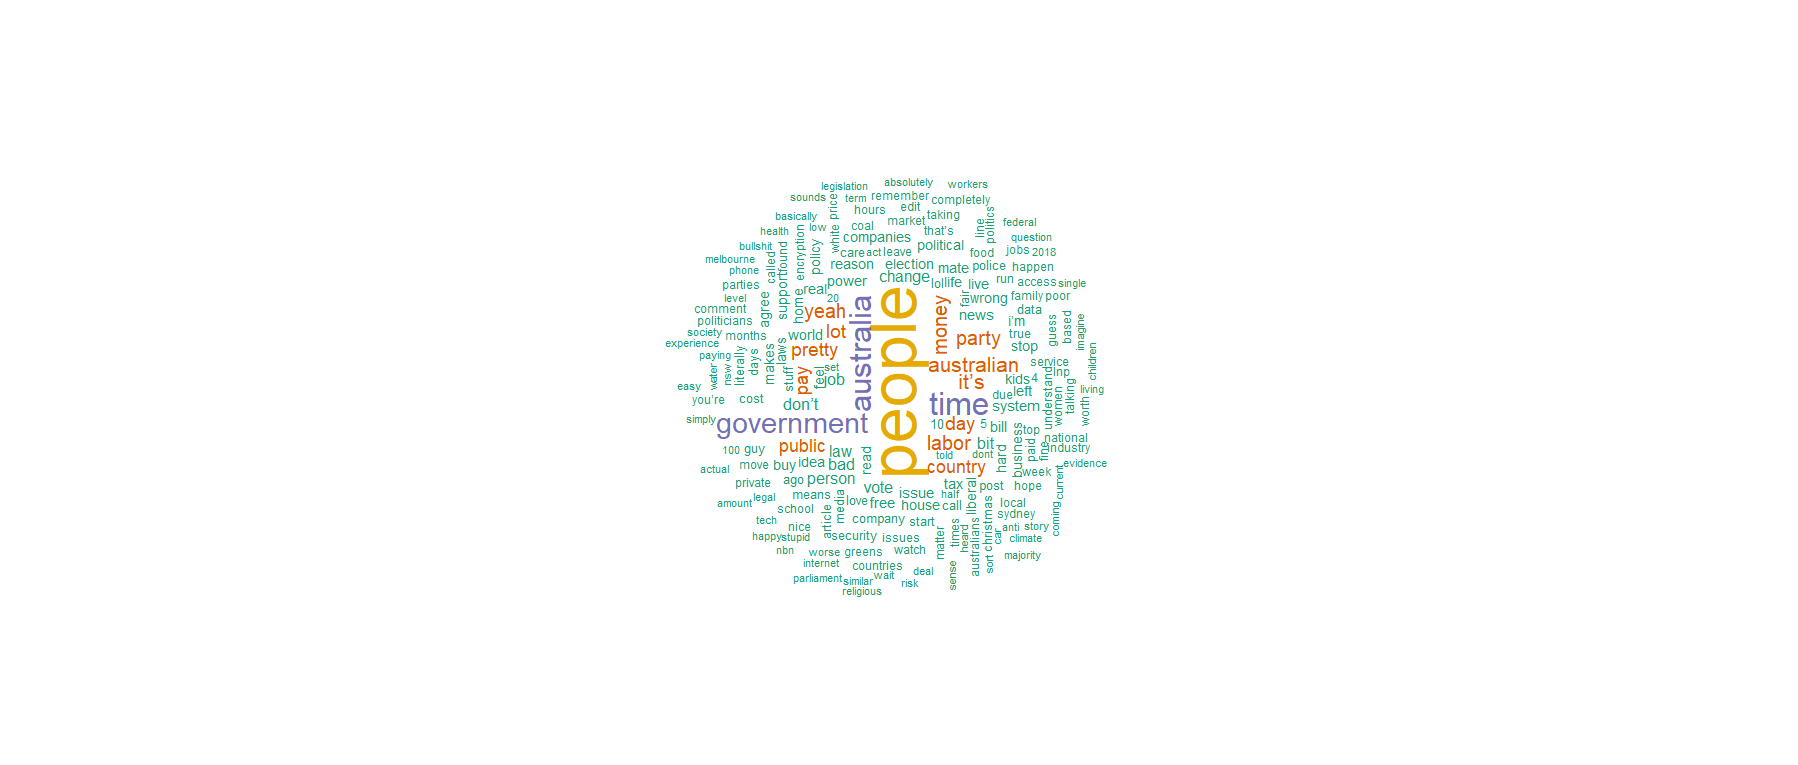
\includegraphics[width=1.0\textwidth]{graphs/australia/wordcloud.png}
    \caption{\textit{Word frequencies on the Australia Subreddit}}
    \label{fig:australia_cloud}
\end{figure}

\begin{figure}[H]
    \centering
    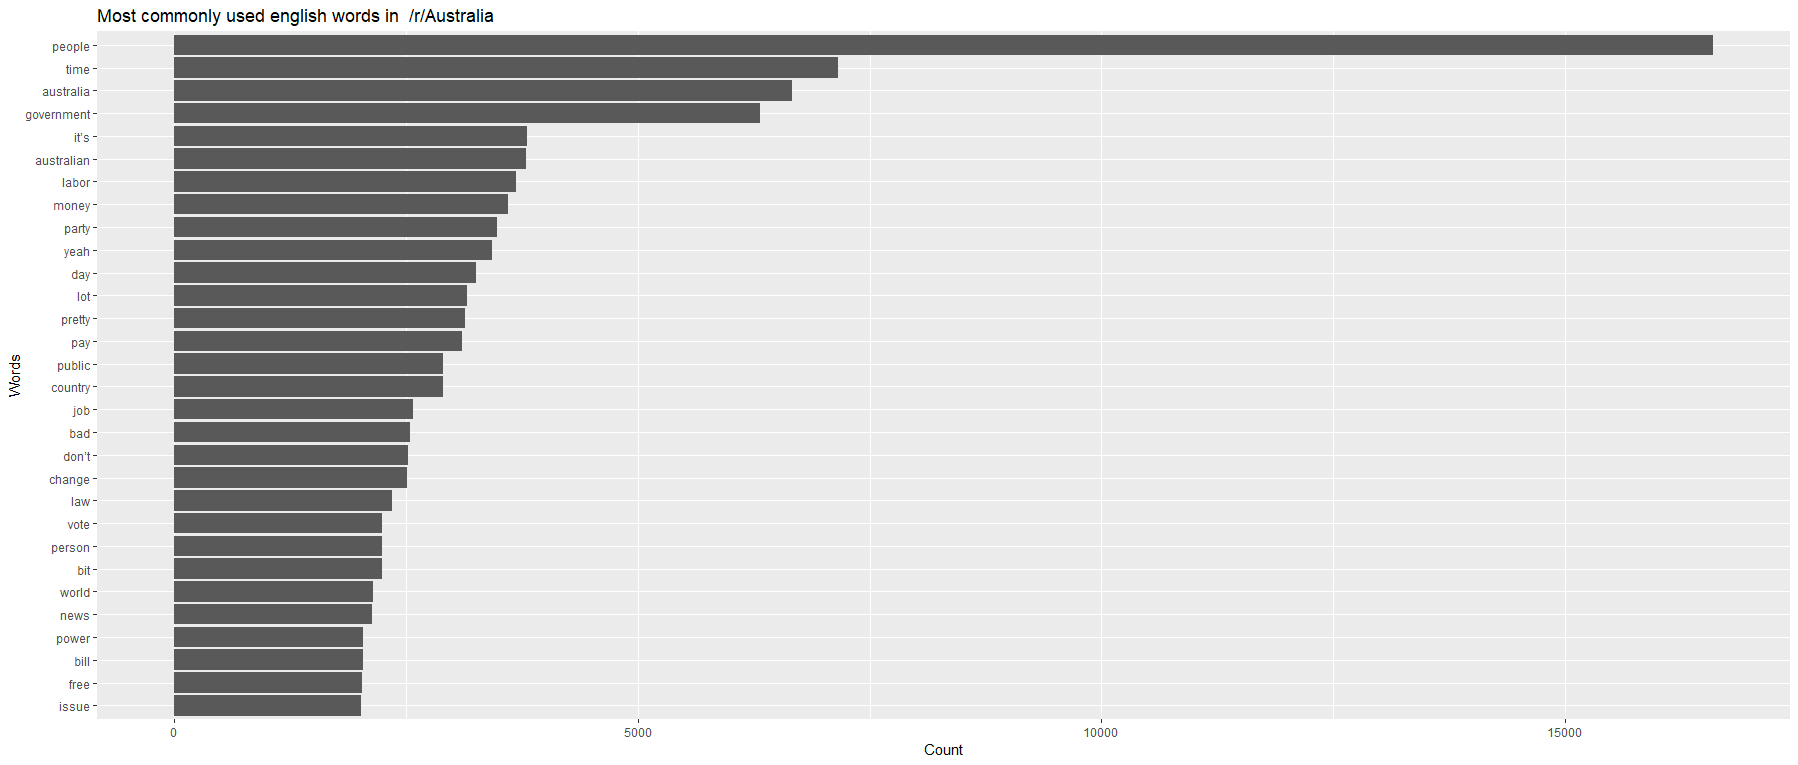
\includegraphics[width=1.0\textwidth]{graphs/australia/wordfreq_canada.png}
    \caption{\textit{Most frequently used terms on /r/australia}}
    \label{fig:australia_wordfreq}
\end{figure}

\section{Canada}
\label{sec:canada}

\begin{figure}[ht]
    \centering
    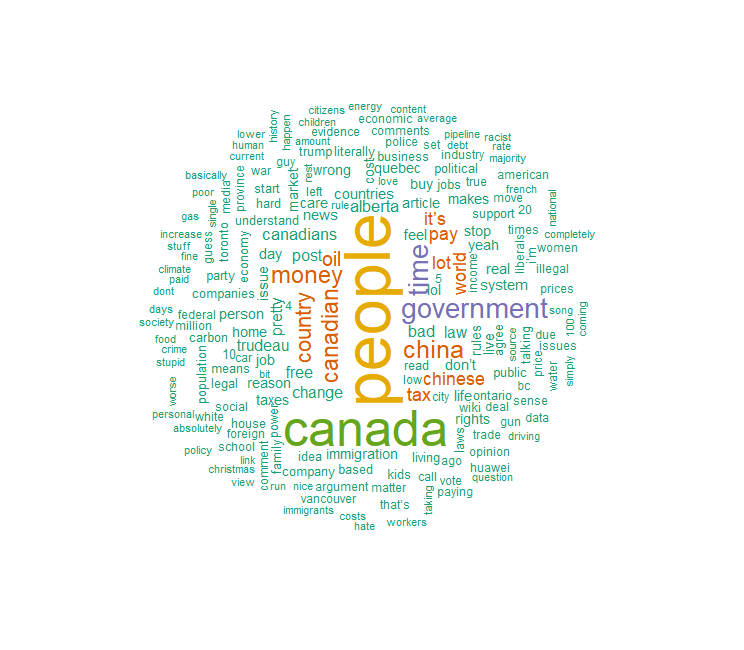
\includegraphics[width=1.0\textwidth]{graphs/Canada/Wordcloud_canada.png}
    \caption{\textit{Word frequencies on the Canada Subreddit}}
    \label{fig:canada_cloud}
\end{figure}

\begin{figure}[H]
    \centering
    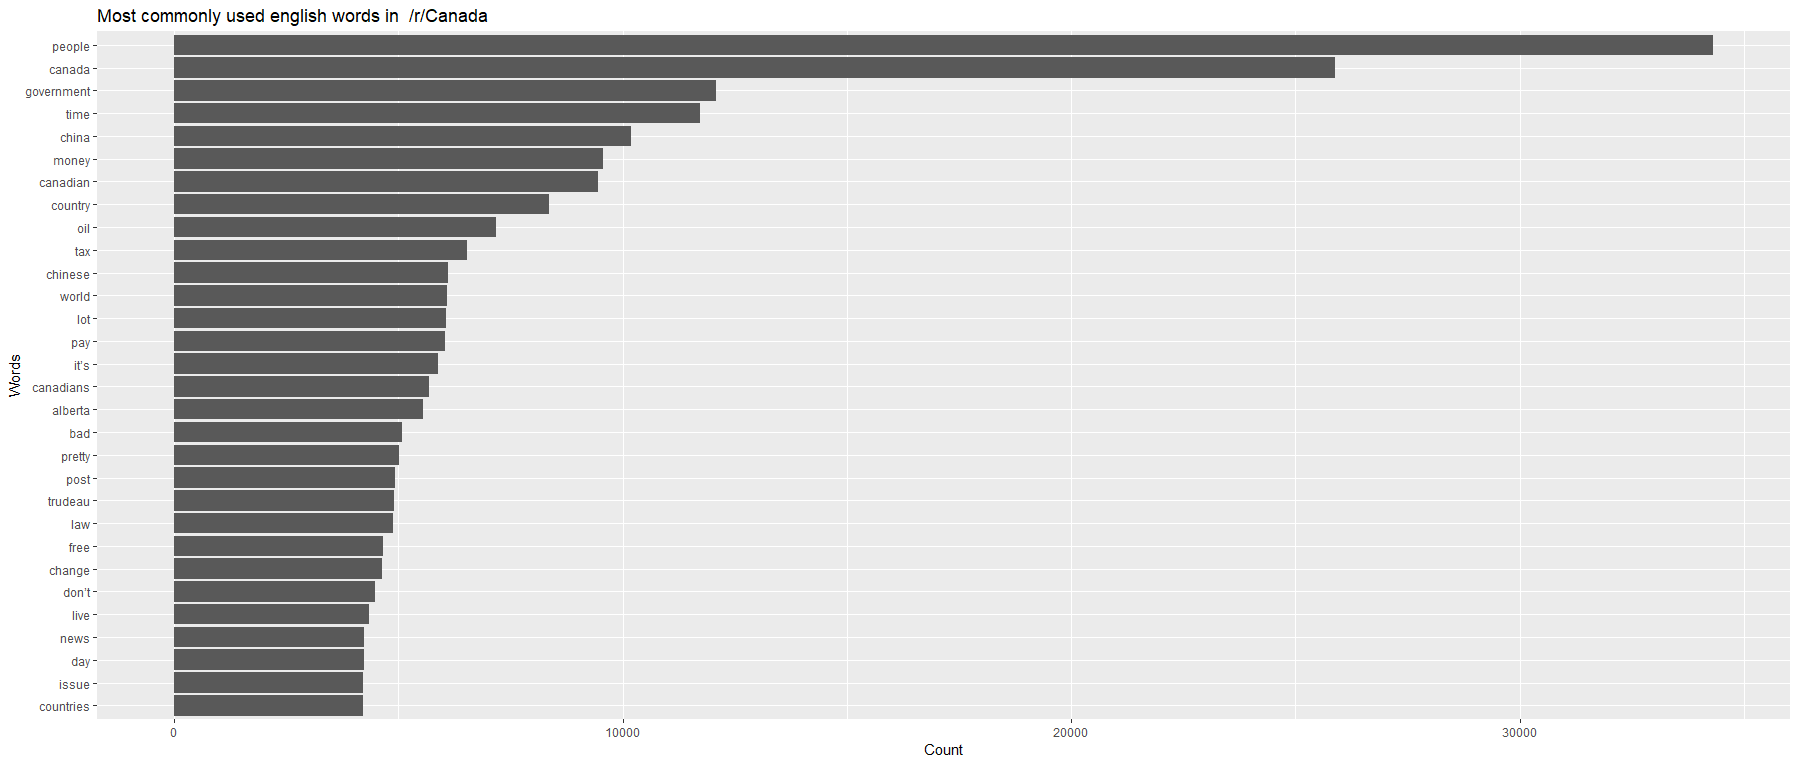
\includegraphics[width=1.0\textwidth]{graphs/Canada/WordFreq_Canada.png}
    \caption{\textit{Most frequently used terms on /r/canada}}
    \label{fig:canada_wordfreq}
\end{figure}

\begin{figure}[H]
    \centering
    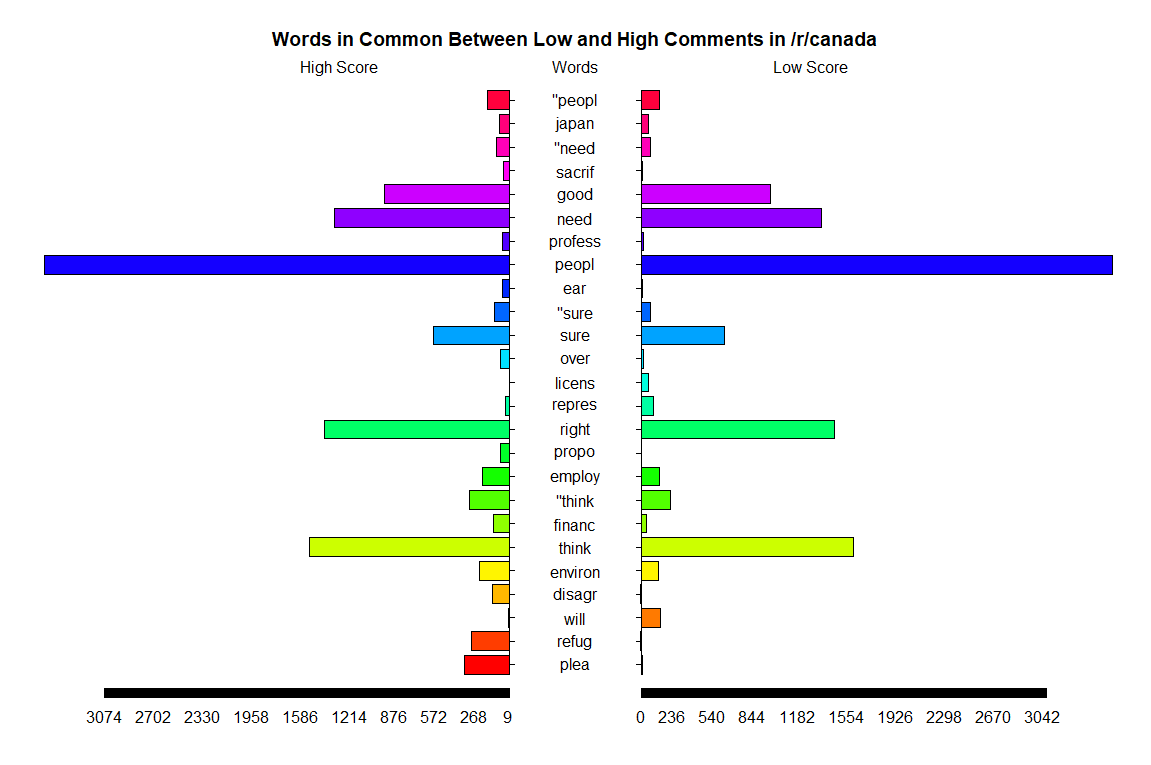
\includegraphics[width=1.0\textwidth]{graphs/Canada/pyramid_canada.png}
    \caption{\textit{Words in common on /r/canada}}
    \label{fig:canada_pyramid}
\end{figure}


\section{DankMemes}
\label{sec:dankmemes}
Some text may be hard to see.

\begin{figure}[ht]
    \centering
    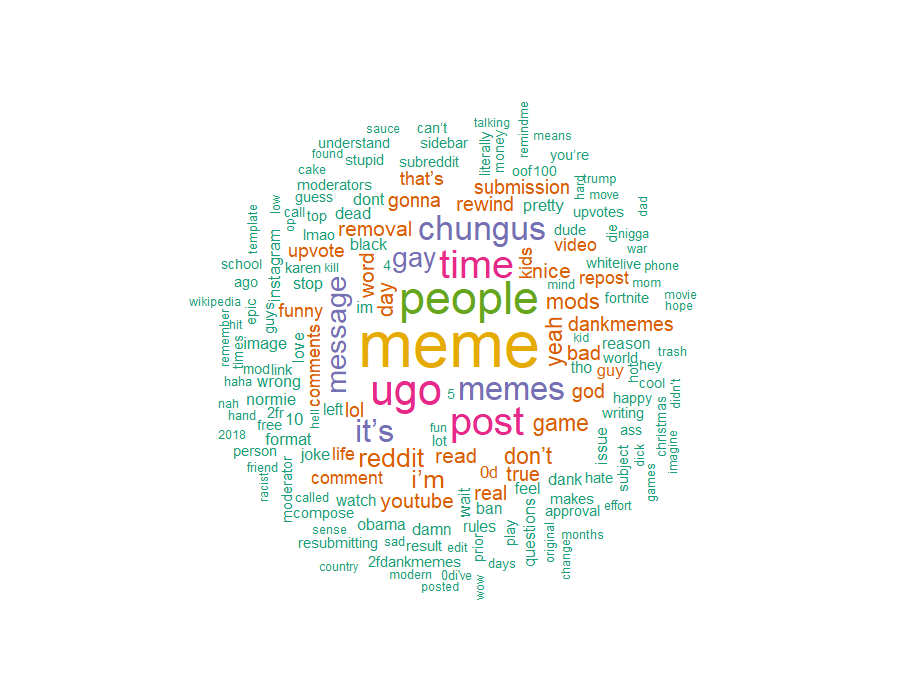
\includegraphics[width=1.0\textwidth]{graphs/DankMemes/wordcloud_DankMemes.png}
    \caption{\textit{Word frequencies on the DankMemes Subreddit}}
    \label{fig:dankmemes_cloud}
\end{figure}

\begin{figure}[H]
    \centering
    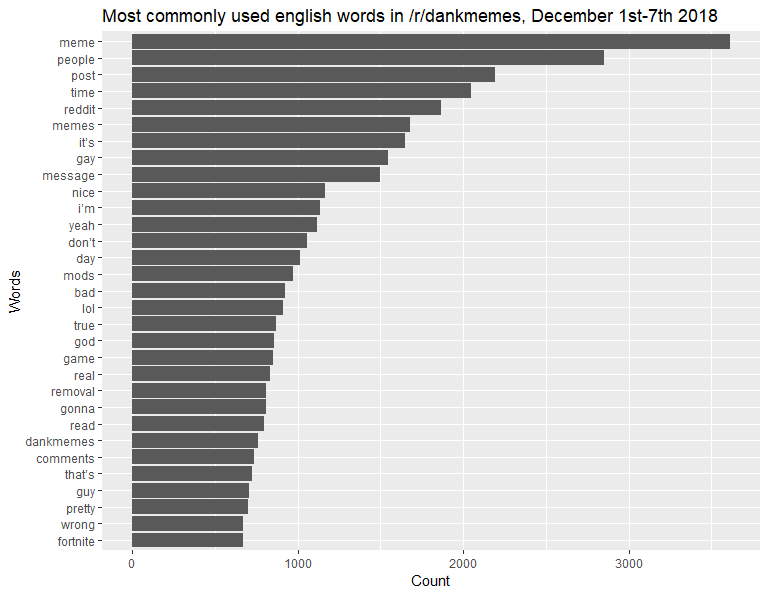
\includegraphics[width=1.0\textwidth]{graphs/DankMemes/wordfreq_rDankMemes.png}
    \caption{\textit{Most frequently used terms on /r/dankmemes}}
    \label{fig:dankmemes_wordfreq}
\end{figure}

\section{Fortnite}
\label{sec:fortnite}
Some text may be hard to see.

\begin{figure}[ht]
    \centering
    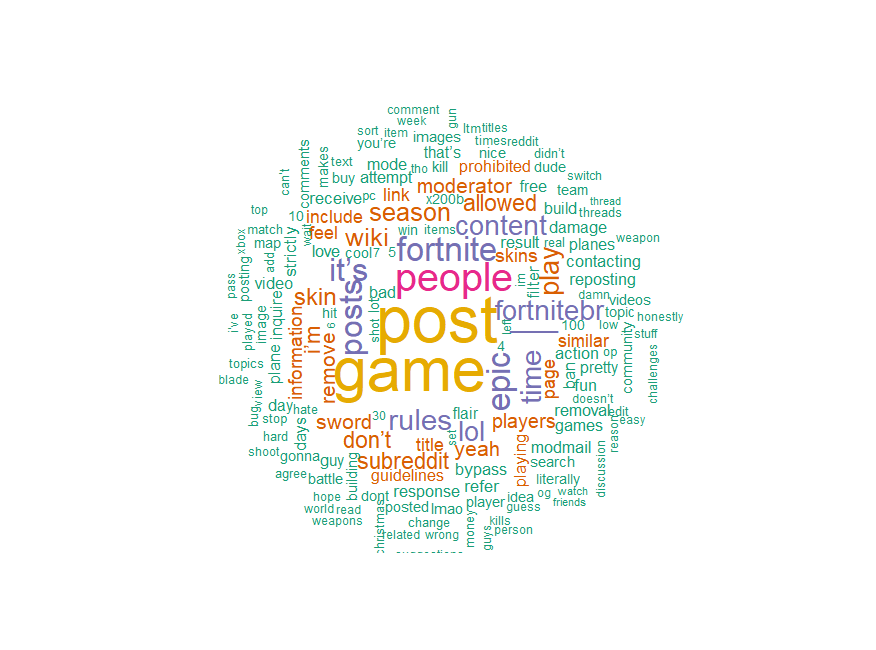
\includegraphics[width=1.0\textwidth]{graphs/Fortnite/wordcloud_Fortnite.png}
    \caption{\textit{Word frequencies on the Fortnite Subreddit}}
    \label{fig:fortnite_cloud}
\end{figure}

\begin{figure}[H]
    \centering
    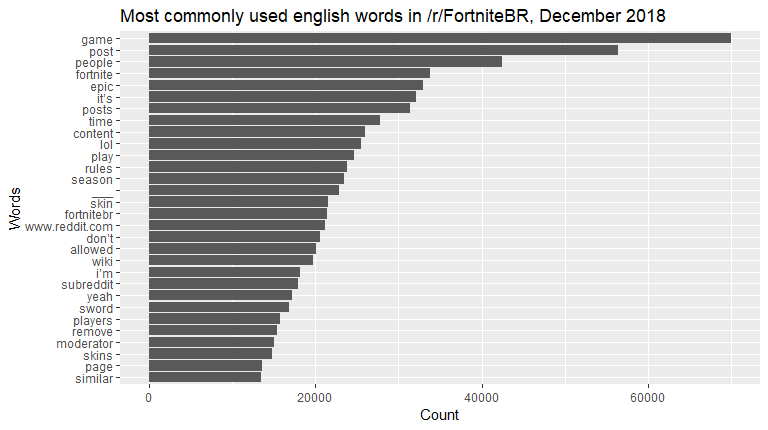
\includegraphics[width=1.0\textwidth]{graphs/Fortnite/WordFreq_FortniteBR.png}
    \caption{\textit{Most frequently used terms on /r/fortnite}}
    \label{fig:fortnite_wordfreq}
\end{figure}

\section{GlobalOffensive}
\label{sec:globaloffensive}
Some text may be hard to see.
\begin{figure}[ht]
    \centering
    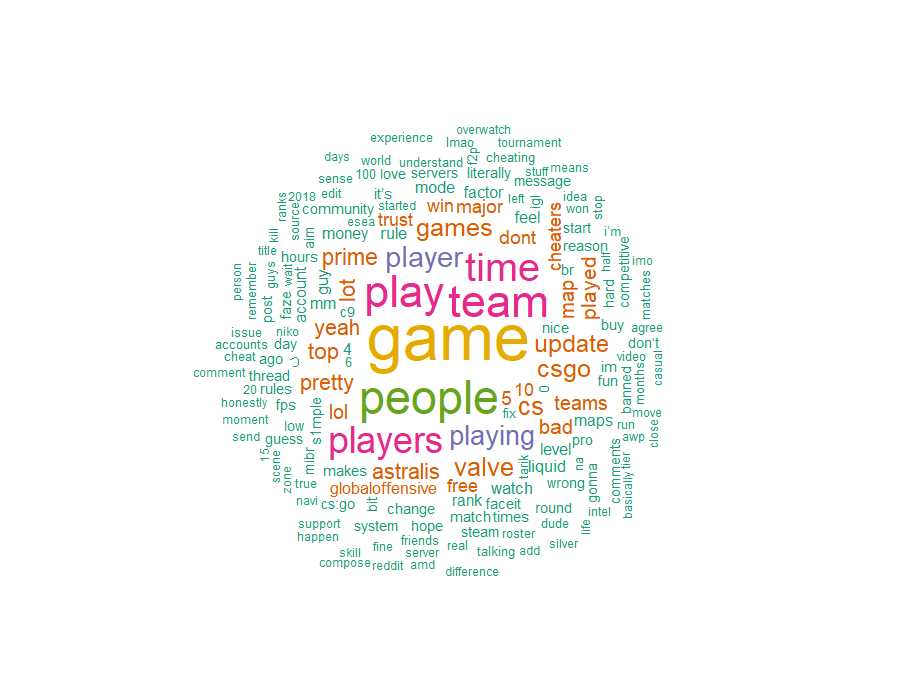
\includegraphics[width=1.0\textwidth]{graphs/GlobalOffensive/wordcloud_rcsgo.png}
    \caption{\textit{Word frequencies on the Global Offensive Subreddit}}
    \label{fig:go_cloud}
\end{figure}

\begin{figure}[H]
    \centering
    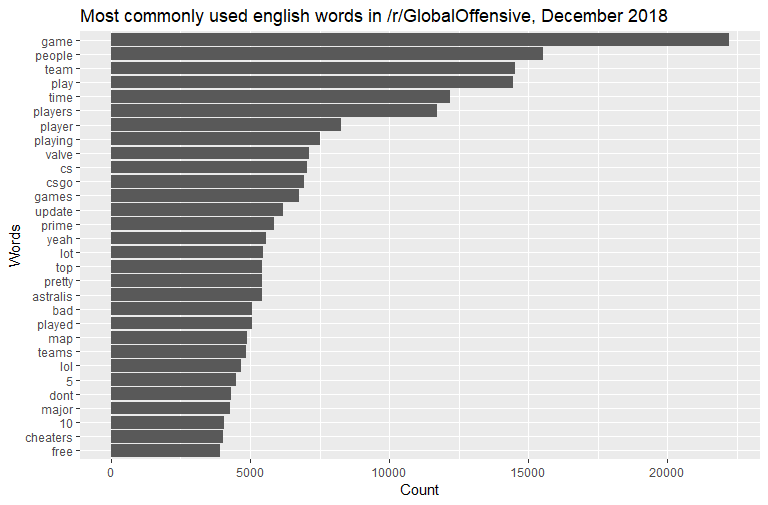
\includegraphics[width=1.0\textwidth]{graphs/GlobalOffensive/WordFreq_GlobalOffensive.png}
    \caption{\textit{Most frequently used terms on /r/globaloffensive}}
    \label{fig:go_wordfreq}
\end{figure}

\begin{figure}[H]
    \centering
    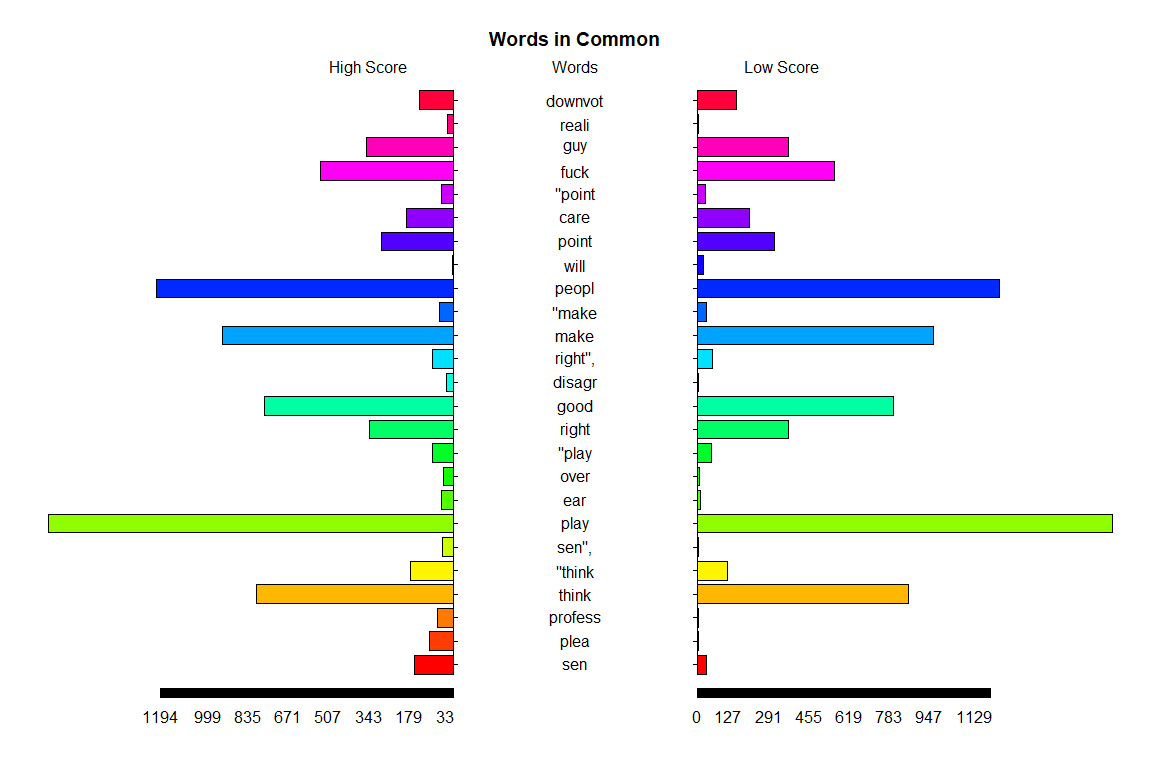
\includegraphics[width=1.0\textwidth]{graphs/GlobalOffensive/Pyramid_GlobalOffensive.png}
    \caption{\textit{Words in common on /r/globaloffensive}}
    \label{fig:go_pyramid}
\end{figure}

\section{LateStageCapitalism}
\label{sec:lsc}
Some text may be hard to see.
\begin{figure}[ht]
    \centering
    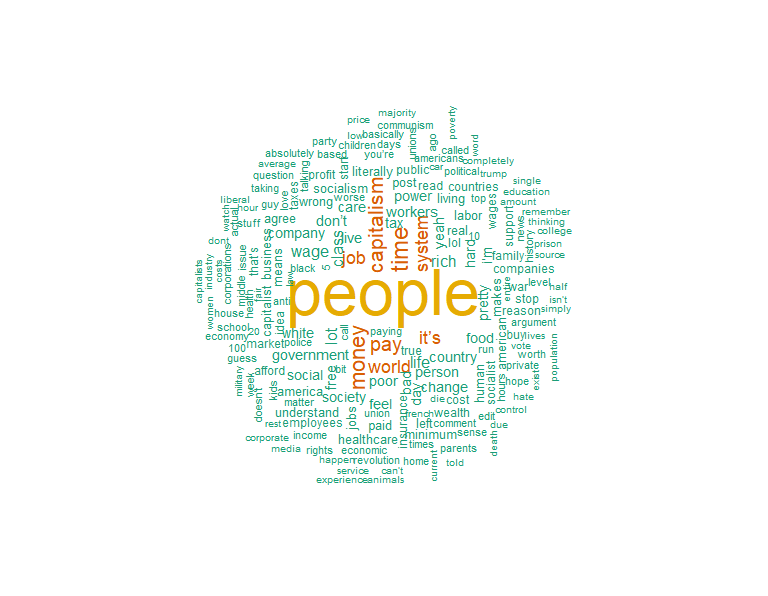
\includegraphics[width=1.0\textwidth]{graphs/LateStageCapitalism/WordCloud_LateStageCapitalism.png}
    \caption{\textit{Word frequencies on the LateStageCapitalism Subreddit}}
    \label{fig:lsc_cloud}
\end{figure}

\begin{figure}[H]
    \centering
    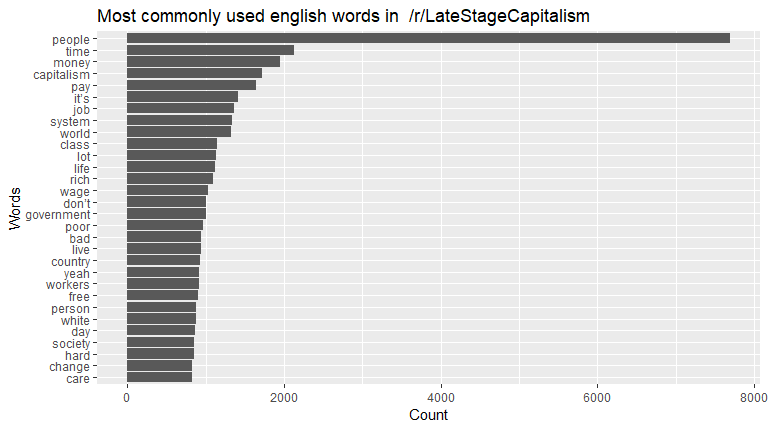
\includegraphics[width=1.0\textwidth]{graphs/LateStageCapitalism/WordFreq_LateStageCapitalism.png}
    \caption{\textit{Most frequently used terms on /r/LateStageCapitalism}}
    \label{fig:lsc_wordfreq}
\end{figure}

\section{Politics}
\label{sec:politics}

\begin{figure}[ht]
    \centering
    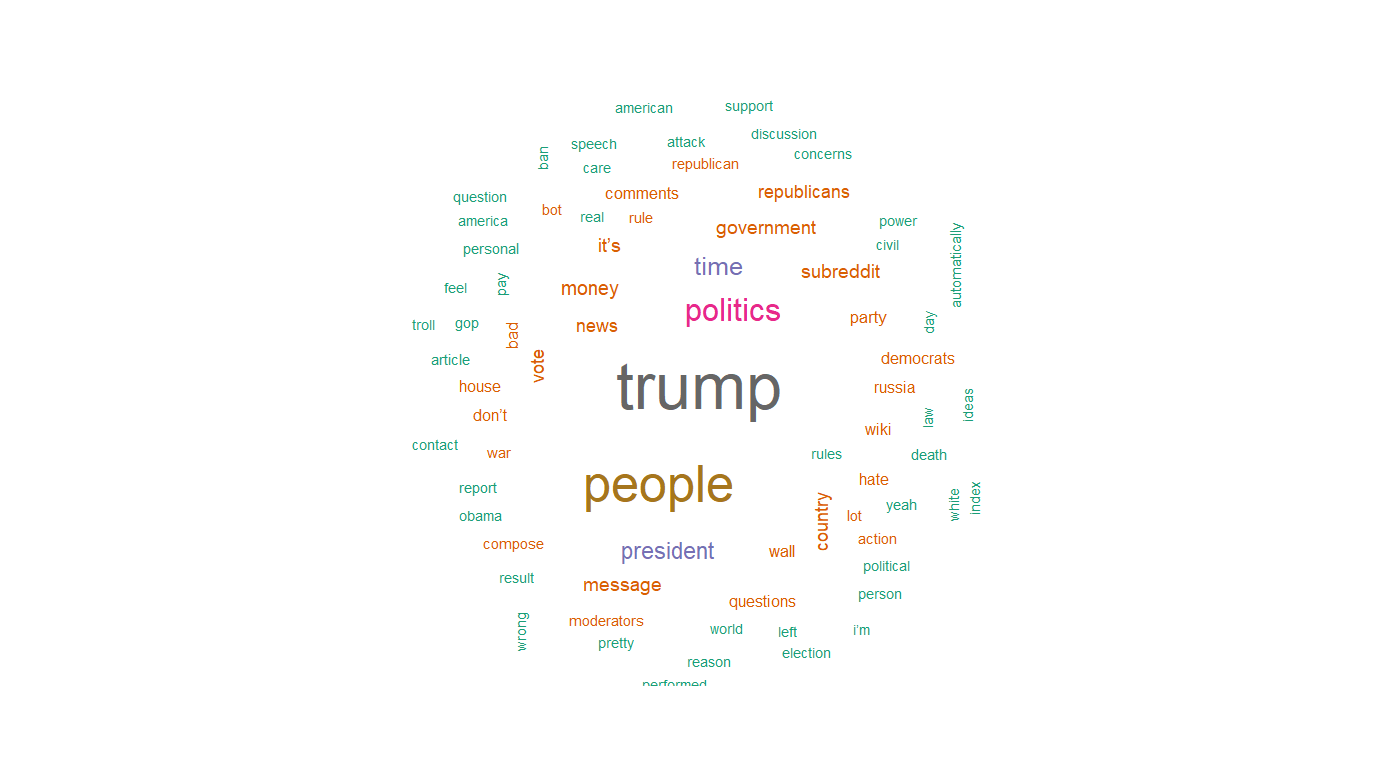
\includegraphics[width=1.0\textwidth]{graphs/politics/Wordcloud_rpolitics.png}
    \caption{\textit{Word frequencies on the Politics Subreddit}}
    \label{fig:politics_cloud}
\end{figure}

\begin{figure}[H]
    \centering
    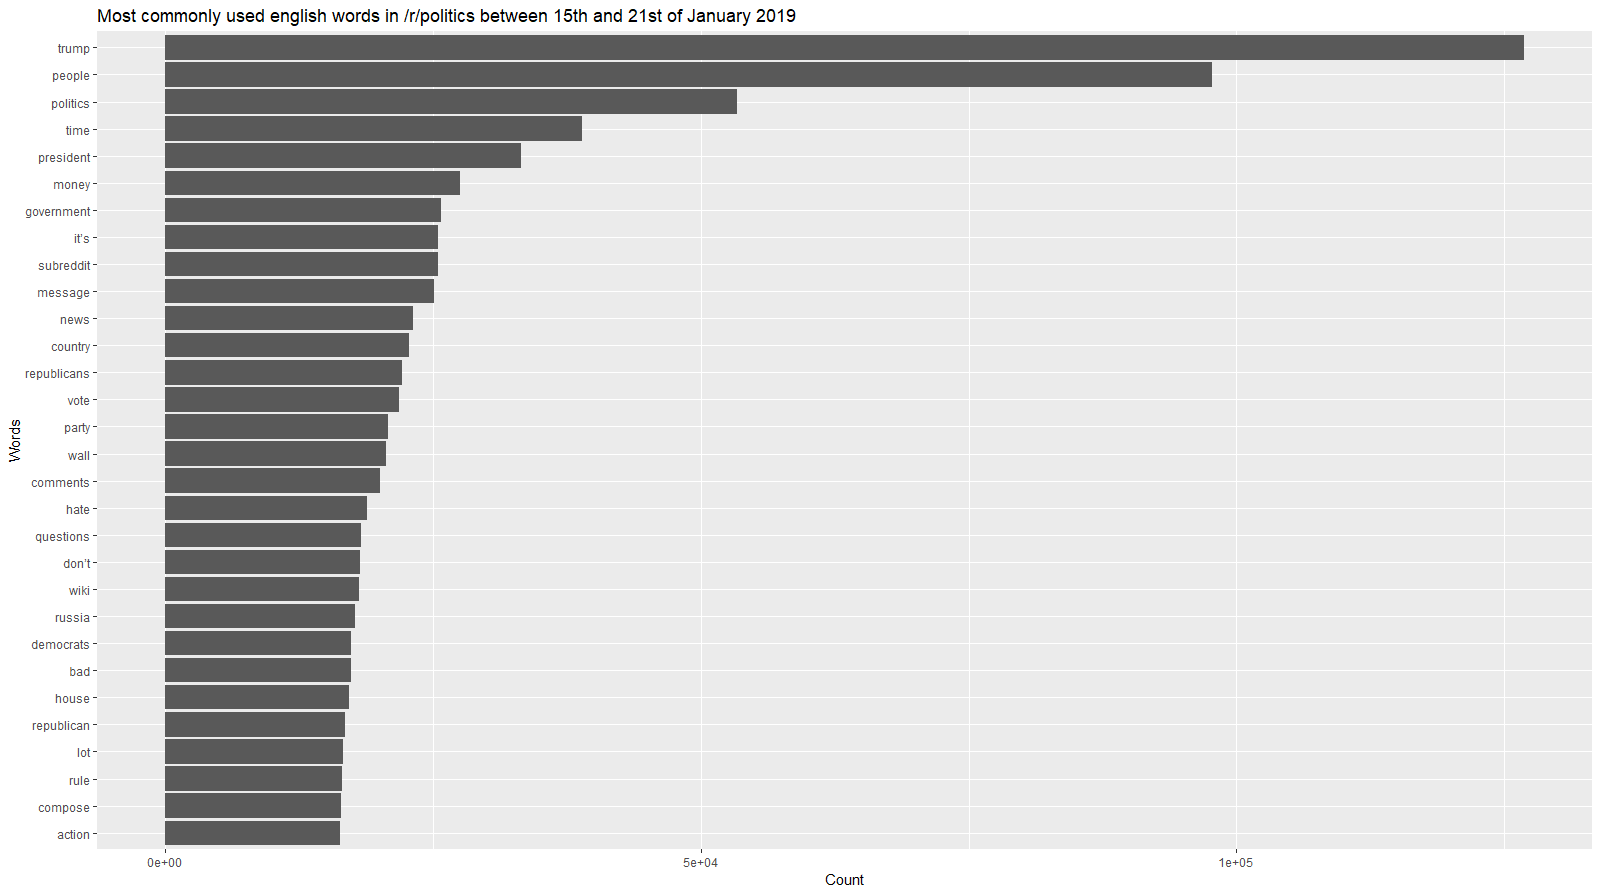
\includegraphics[width=1.0\textwidth]{graphs/politics/Bargraph_rPolitics.png}
    \caption{\textit{Most frequently used terms on /r/Politics}}
    \label{fig:politics_wordfreq}
\end{figure}

\section{PUBG}
Some text may be hard to see.
\label{sec:pubg}
\begin{figure}[ht]
    \centering
    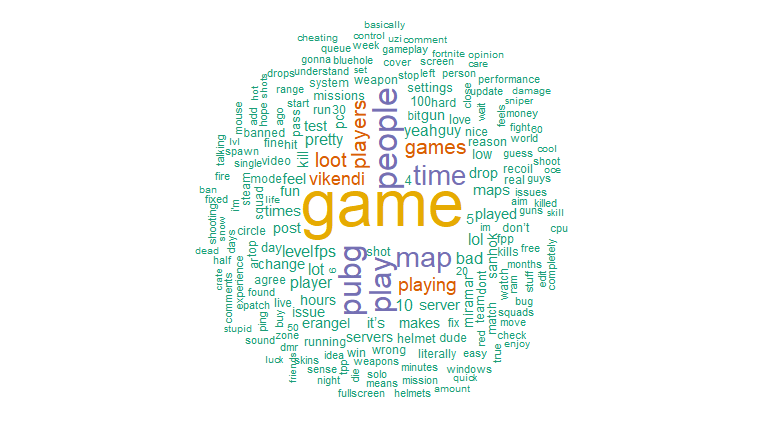
\includegraphics[width=1.0\textwidth]{graphs/PUBG/WordCloud_PUBG.png}
    \caption{\textit{Word frequencies on the PUBG Subreddit}}
    \label{fig:pubg_cloud}
\end{figure}

\begin{figure}[H]
    \centering
    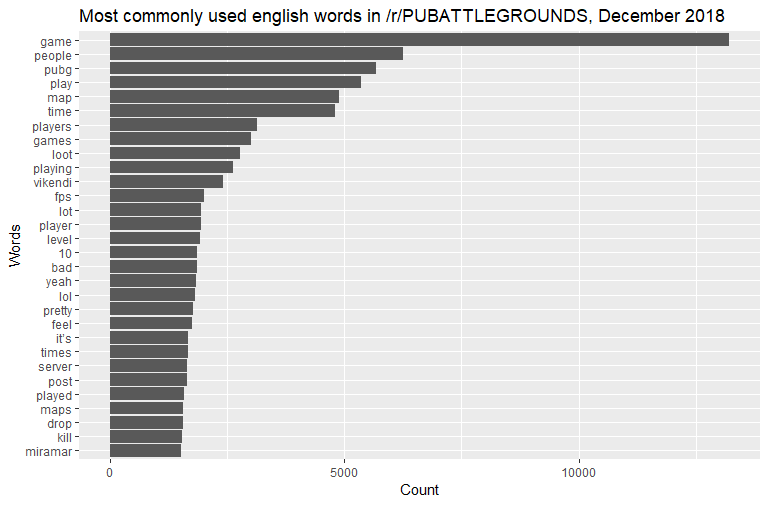
\includegraphics[width=1.0\textwidth]{graphs/PUBG/WordFreq_PUBG.png}
    \caption{\textit{Most frequently used terms on /r/pubg}}
    \label{fig:pubg_wordfreq}
\end{figure}

\section{The\_Donald}
Some text may be hard to see.
\label{sec:thedonald}

\begin{figure}[ht]
    \centering
    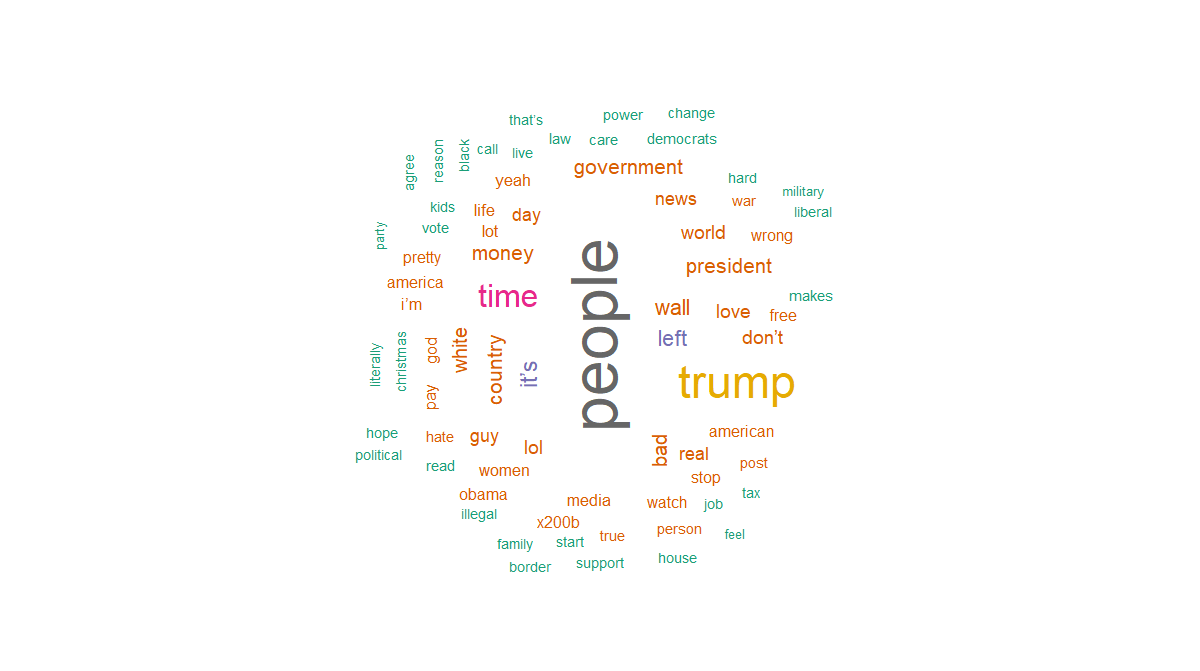
\includegraphics[width=1.0\textwidth]{graphs/The_Donald/Wallcloud_the_donald.png}
    \caption{\textit{Word frequencies on the The_Donald Subreddit}}
    \label{fig:thedonald_cloud}
\end{figure}

\begin{figure}[H]
    \centering
    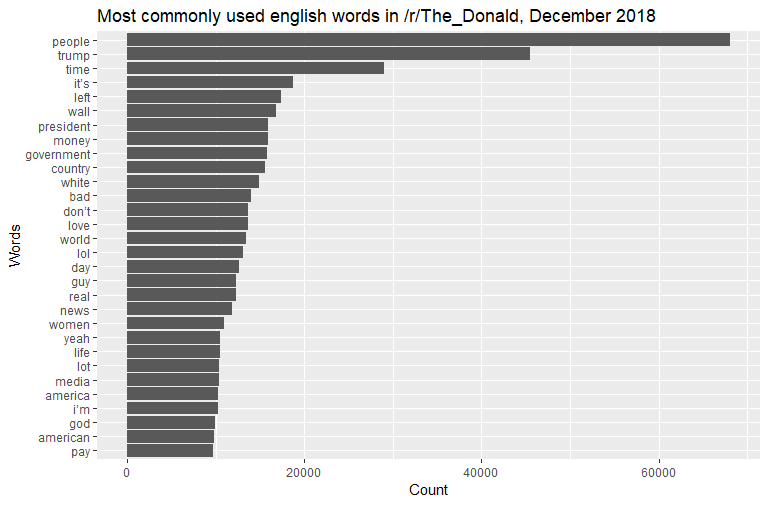
\includegraphics[width=1.0\textwidth]{graphs/The_Donald/WordFreq_TheDonald.png}
    \caption{\textit{Most frequently used terms on /r/The_Donald}}
    \label{fig:thedonald_wordfreq}
\end{figure}

\section{United Kingdom}
Some text may be hard to see.
\label{sec:uk}

\begin{figure}[ht]
    \centering
    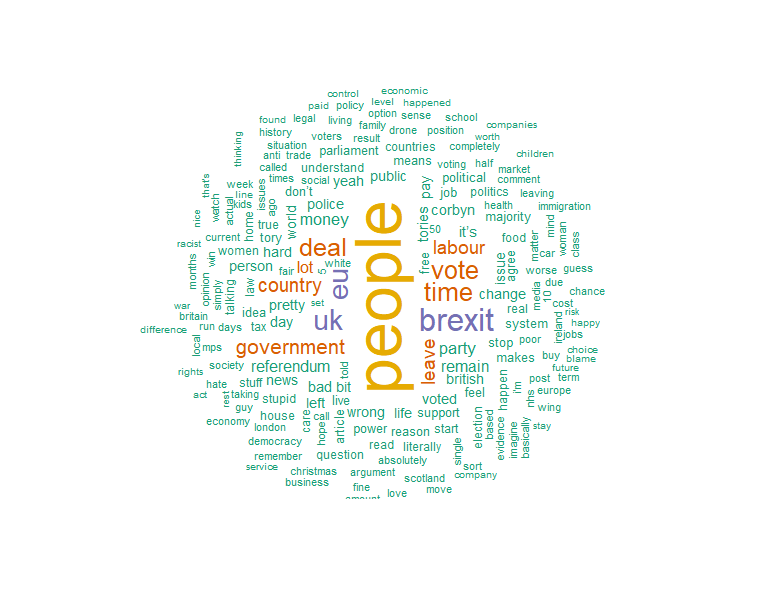
\includegraphics[width=1.0\textwidth]{graphs/UnitedKingdom/WordCloud_UK.png}
    \caption{\textit{Word frequencies on the UnitedKingdom Subreddit}}
    \label{fig:uk_cloud}
\end{figure}

\begin{figure}[H]
    \centering
    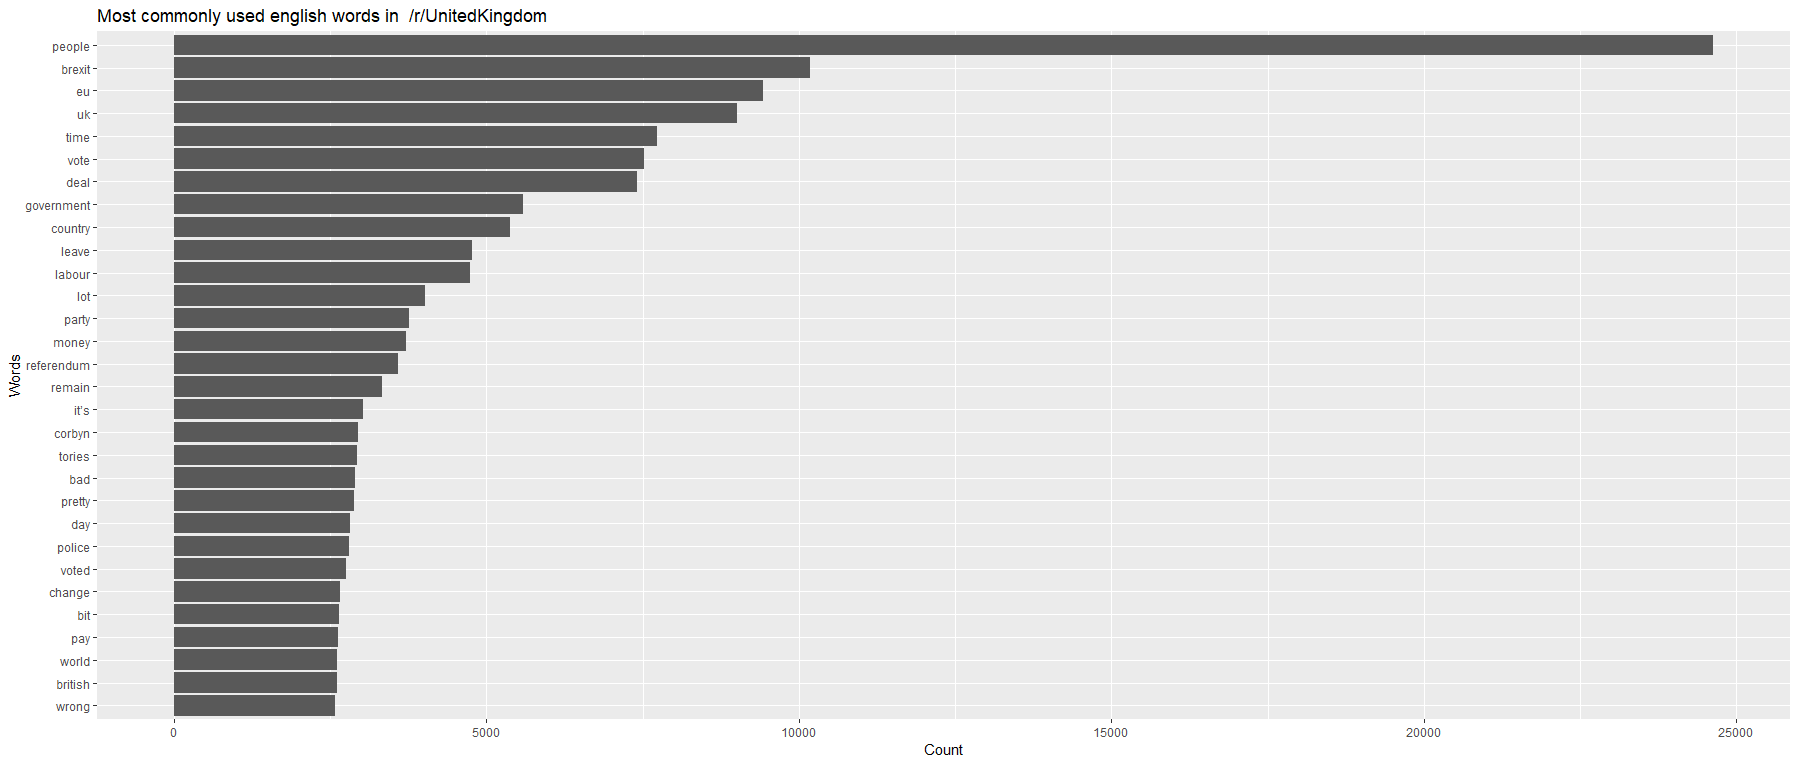
\includegraphics[width=1.0\textwidth]{graphs/UnitedKingdom/WordFreq_UK.png}
    \caption{\textit{Most frequently used terms on /r/UnitedKingdom}}
    \label{fig:uk_wordfreq}
\end{figure}

\section{General}
Some text may be hard to see.
\begin{figure}[ht]
    \centering
    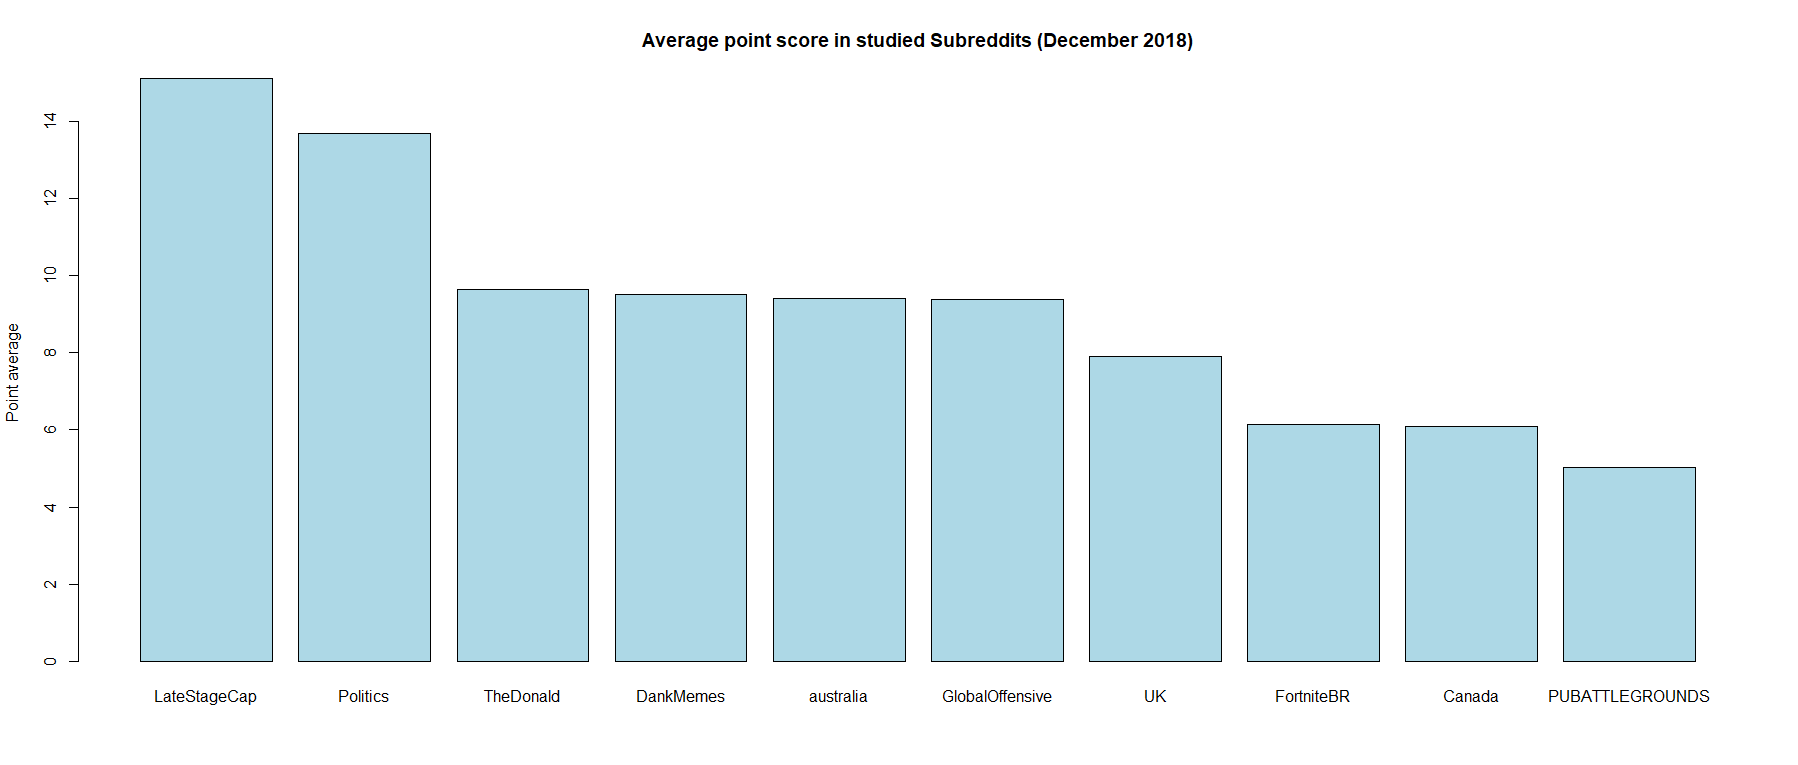
\includegraphics[width=1.0\textwidth]{graphs/Average_meanscore.png}
    \caption{\textit{Average Mean Score on studied Subreddits}}
    \label{fig:avgScore}
\end{figure}

\begin{figure}[H]
    \centering
    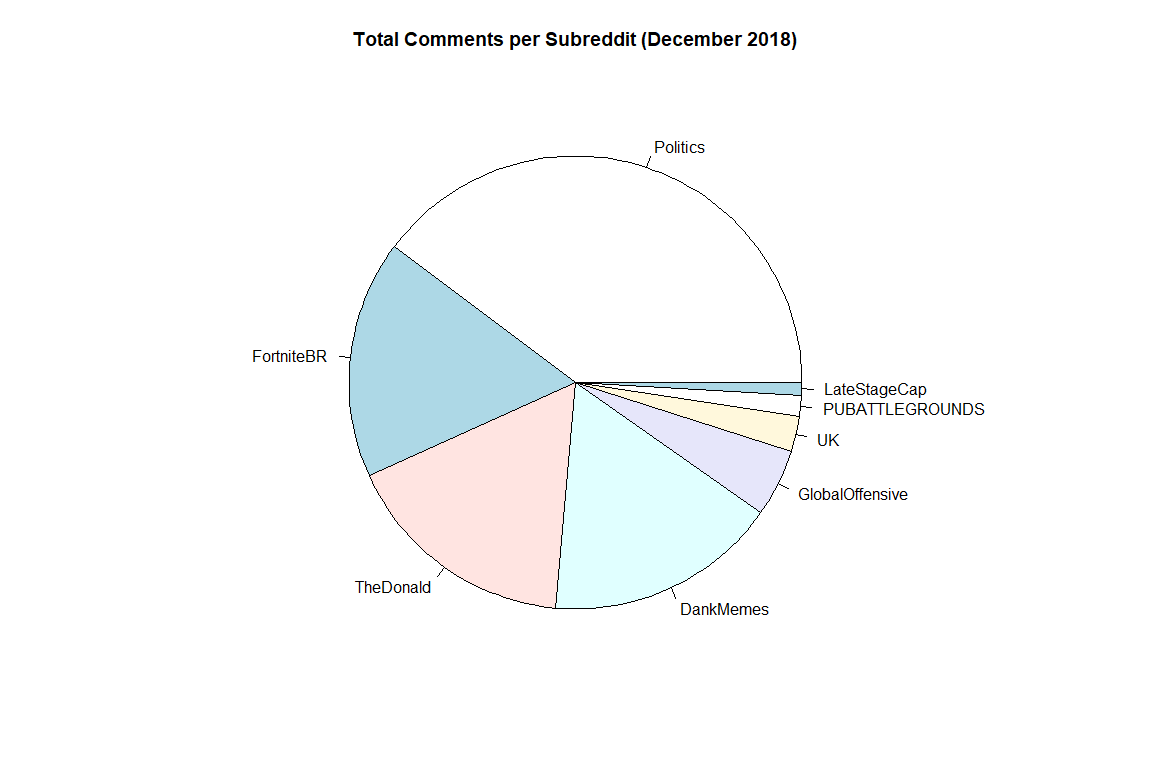
\includegraphics[width=1.0\textwidth]{graphs/piechart_counts.png}
    \caption{\textit{Pi chart of total comments on studied Subreddits}}
    \label{fig:pichart}
\end{figure}

\begin{figure}[H]
    \centering
    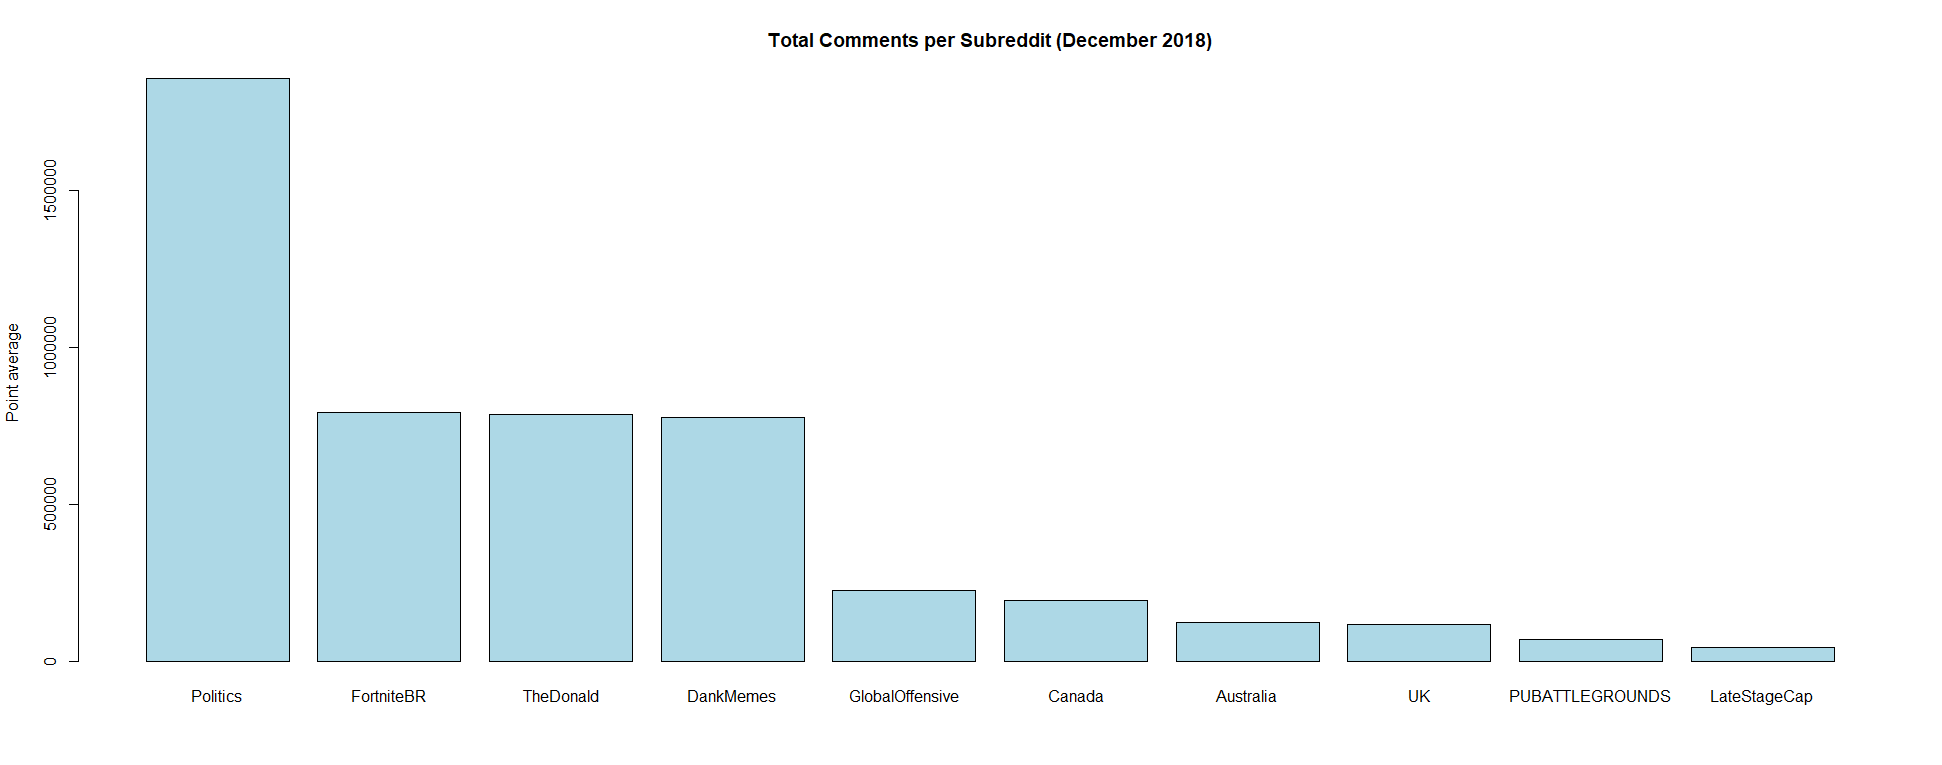
\includegraphics[width=1.0\textwidth]{graphs/BarGraph_TotalComments.png}
    \caption{\textit{Total comments on each studied Subreddit}}
    \label{fig:pichart}
\end{figure}



\end{document} %NOTE: END of document, nothing after this point
